\noindent
Figures~\ref{fig:pwflag0_full}--\ref{fig:pwflag5_full} provide the full variable-by-variable
checks for each reconstructed particle category that contributes to thrust. In each case, the
same observable set is shown to keep the detector-level validation uniform across categories:
angular acceptance, momentum scale, and quality-related variables are all checked before
constructing event-shape observables.

\begin{figure}[t!]
\centering
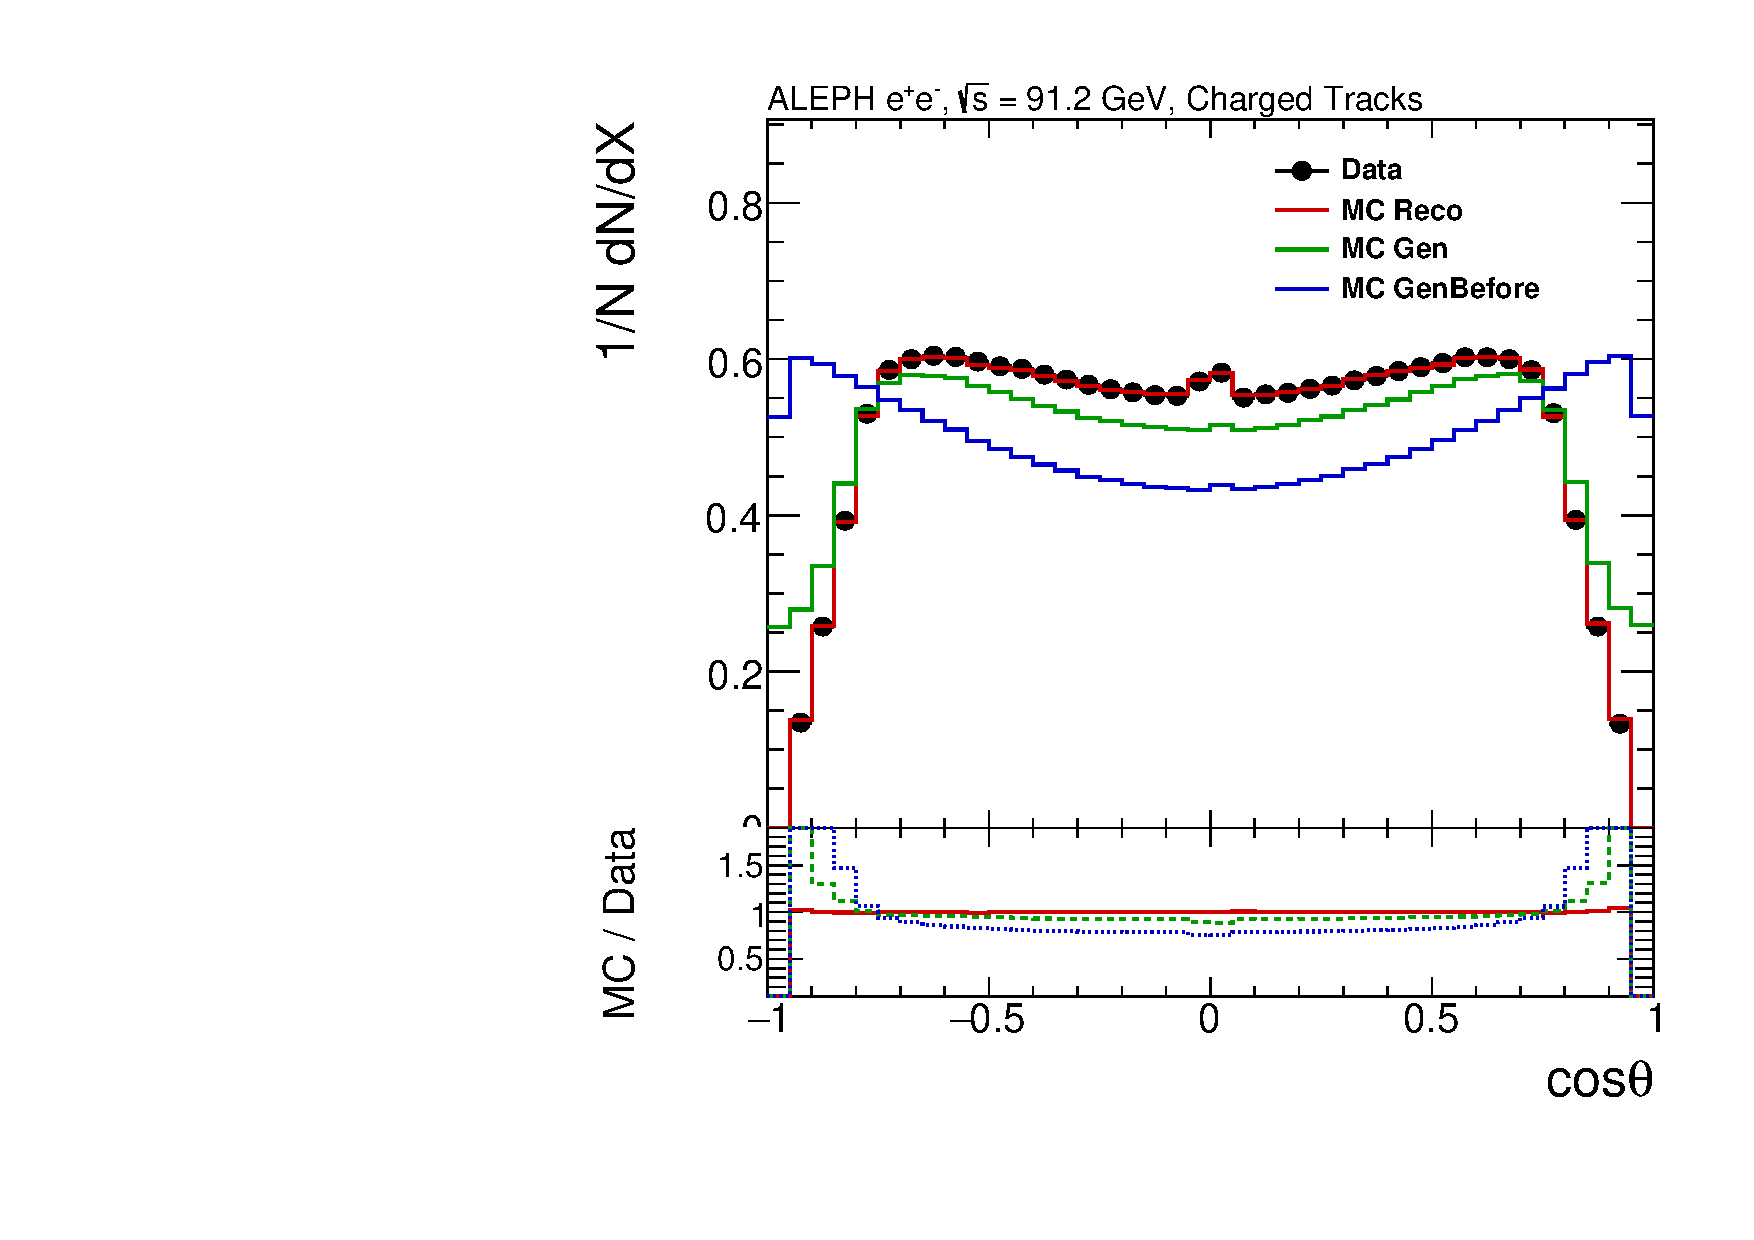
\includegraphics[width=0.325\textwidth]{../Studies/PreliminaryResult/2026-02-17_thrust_iter5/pwflag_kinematics/pwflag0_cosTheta.pdf}
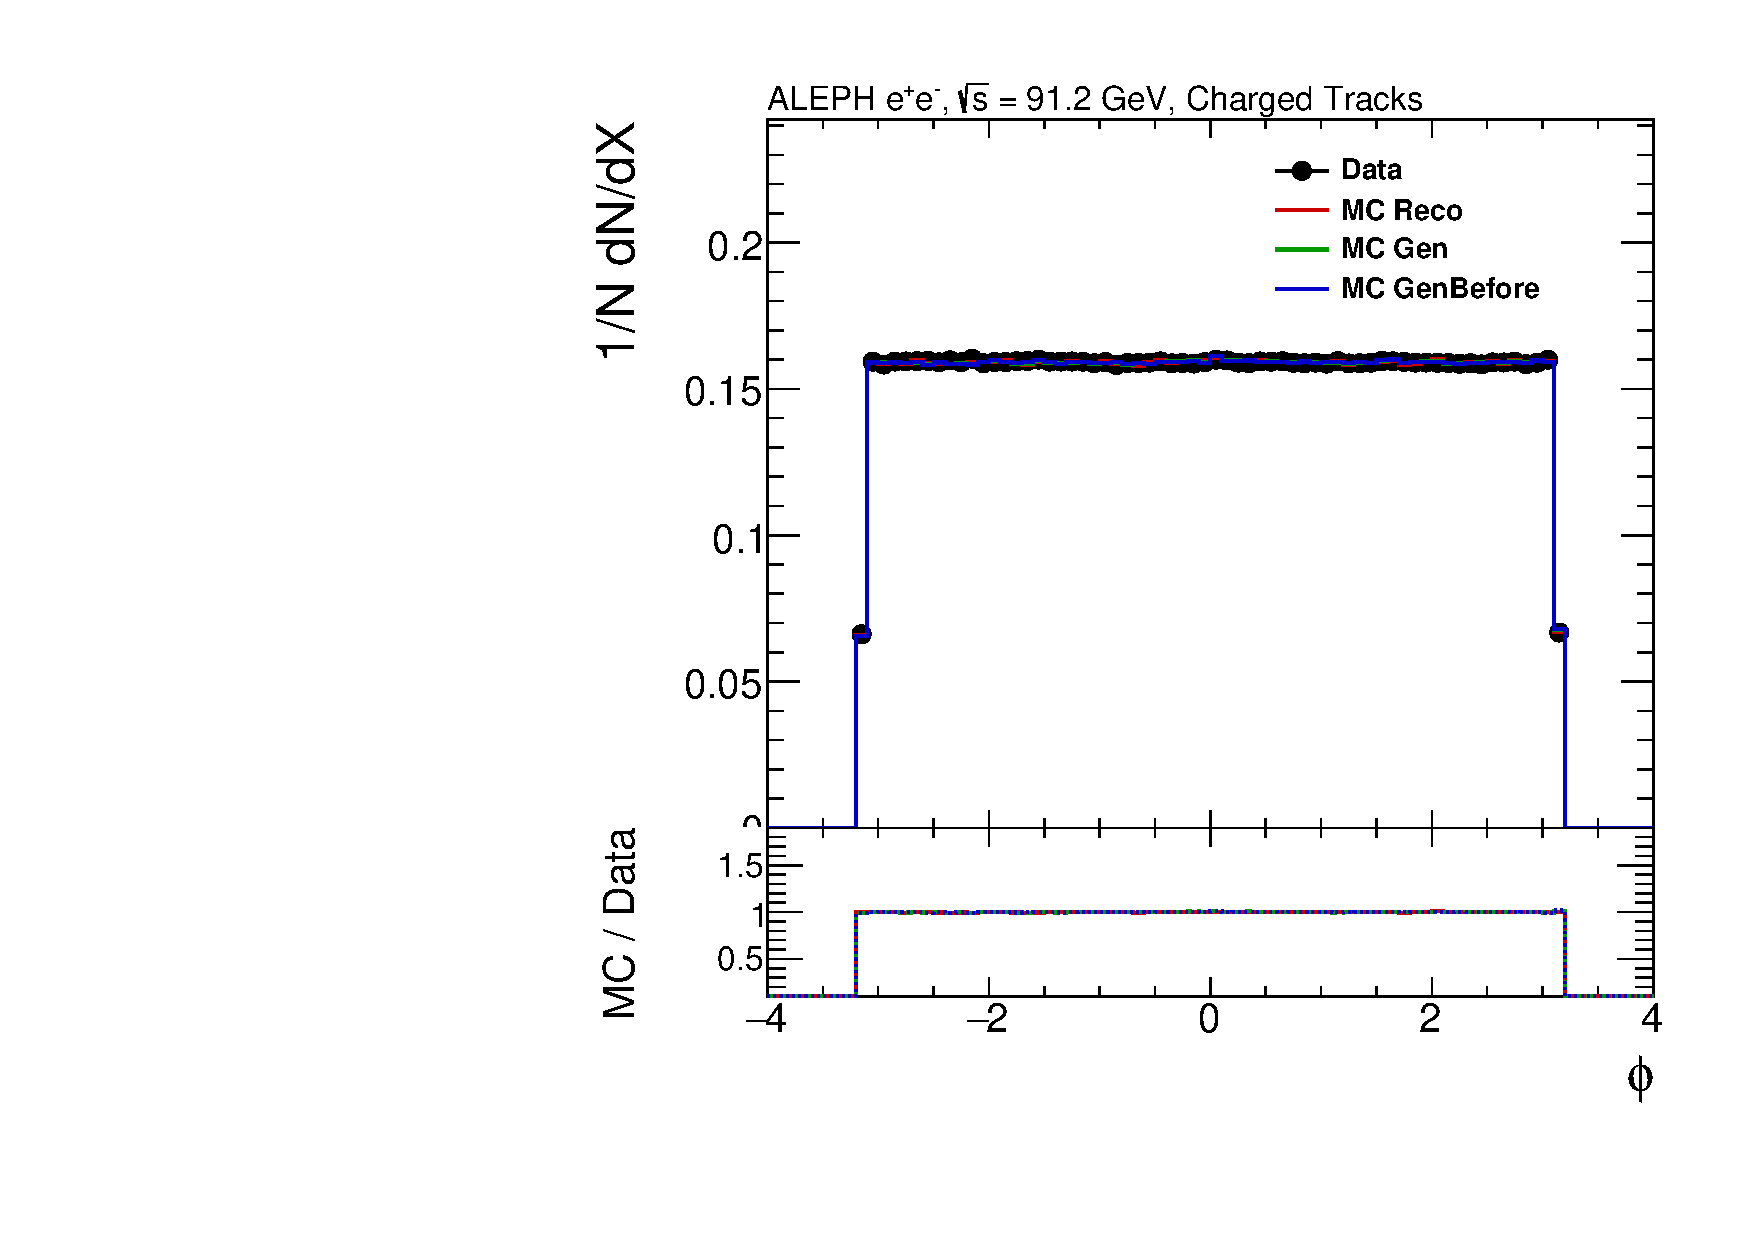
\includegraphics[width=0.325\textwidth]{../Studies/PreliminaryResult/2026-02-17_thrust_iter5/pwflag_kinematics/pwflag0_phi.pdf}
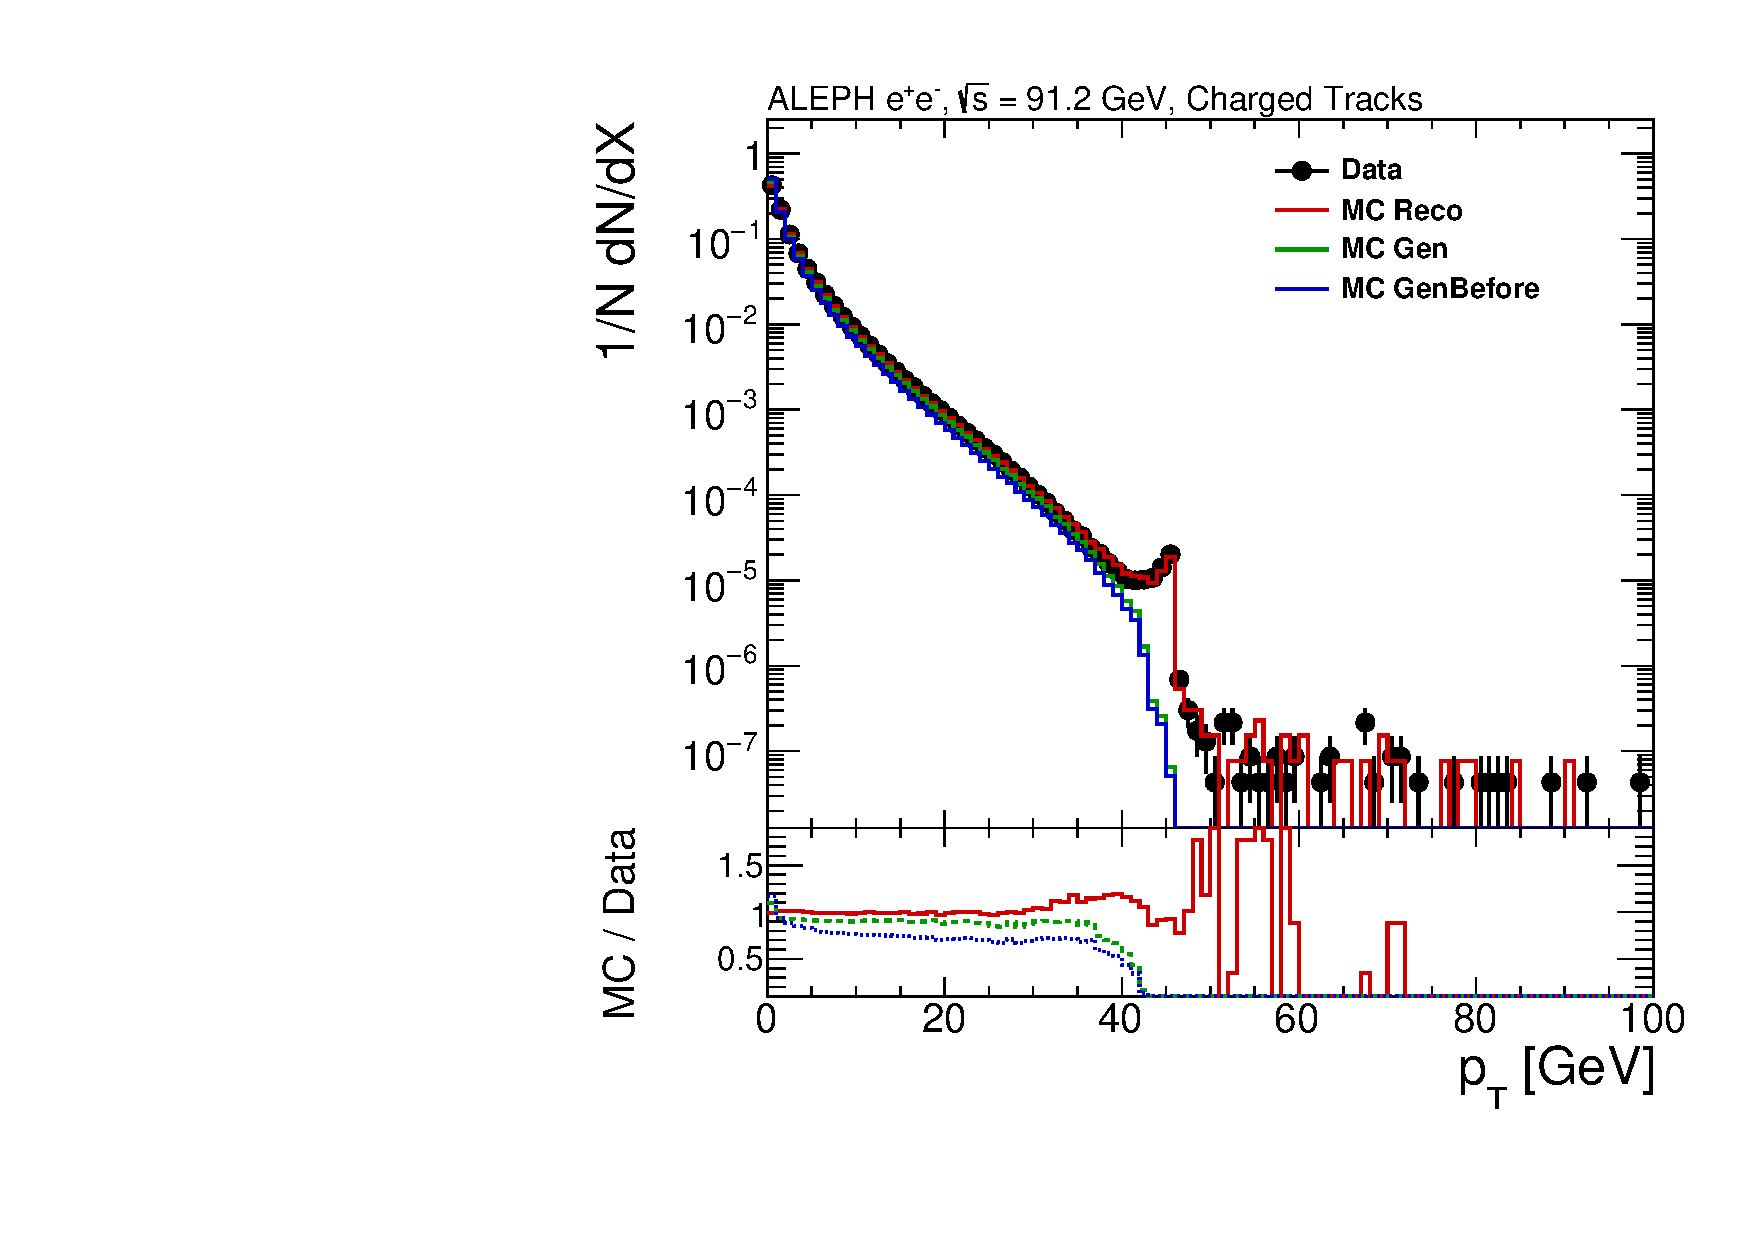
\includegraphics[width=0.325\textwidth]{../Studies/PreliminaryResult/2026-02-17_thrust_iter5/pwflag_kinematics/pwflag0_pt.pdf}
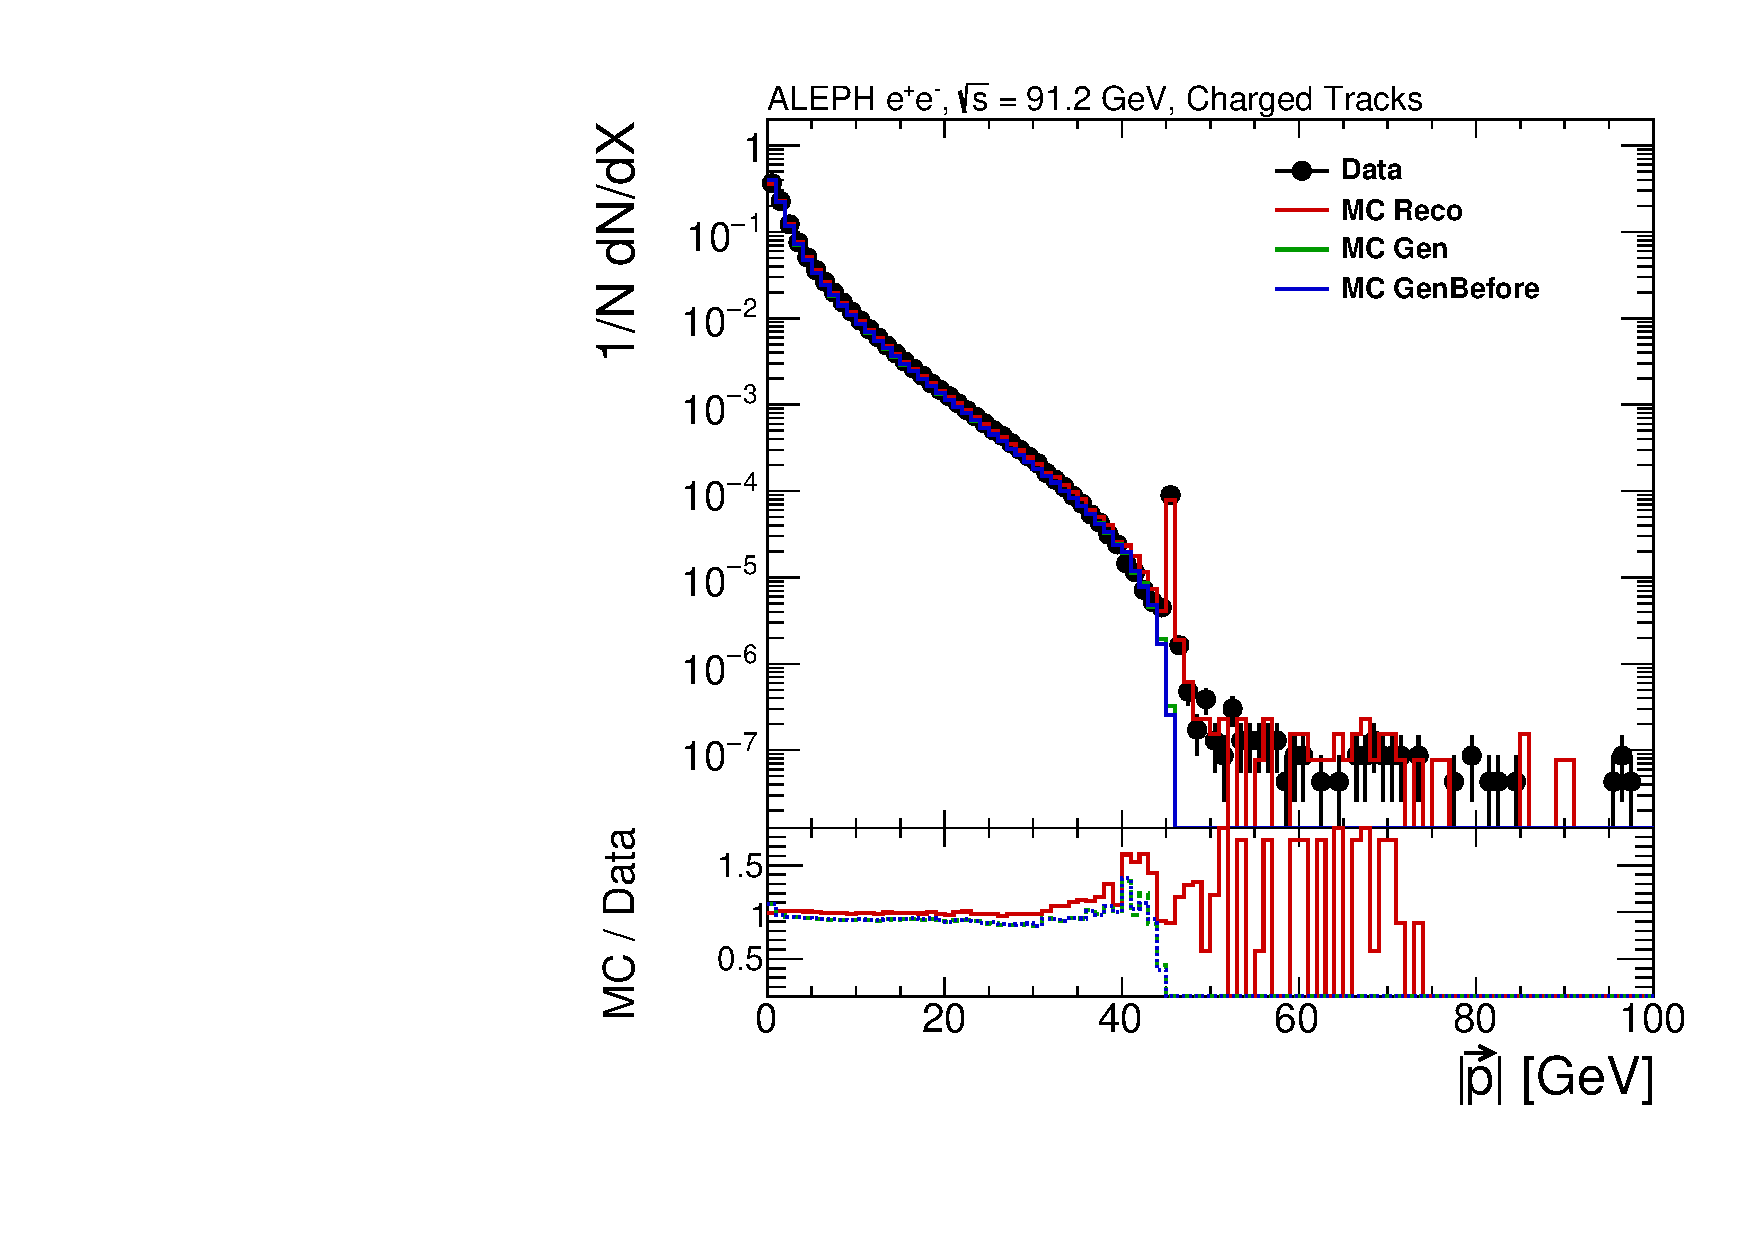
\includegraphics[width=0.325\textwidth]{../Studies/PreliminaryResult/2026-02-17_thrust_iter5/pwflag_kinematics/pwflag0_pmag.pdf}
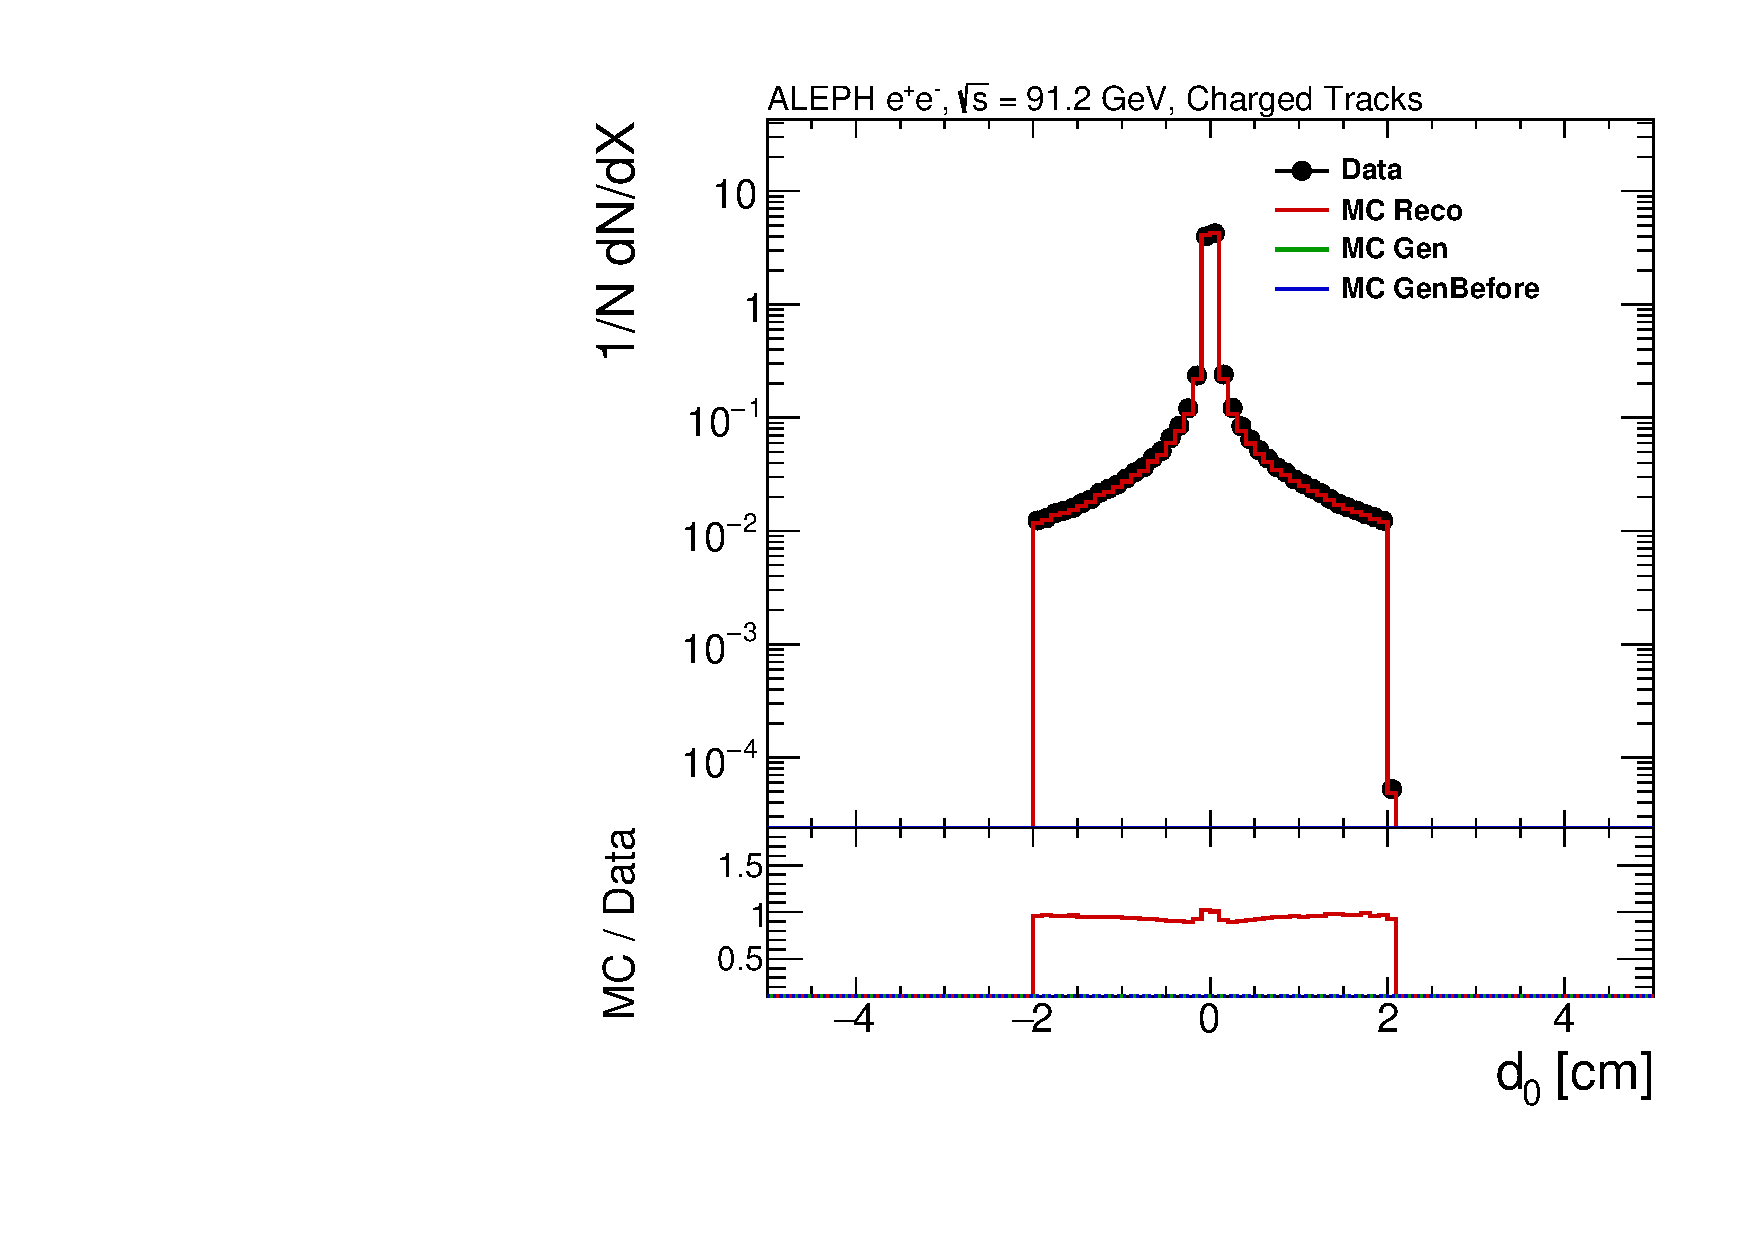
\includegraphics[width=0.325\textwidth]{../Studies/PreliminaryResult/2026-02-17_thrust_iter5/pwflag_kinematics/pwflag0_d0.pdf}
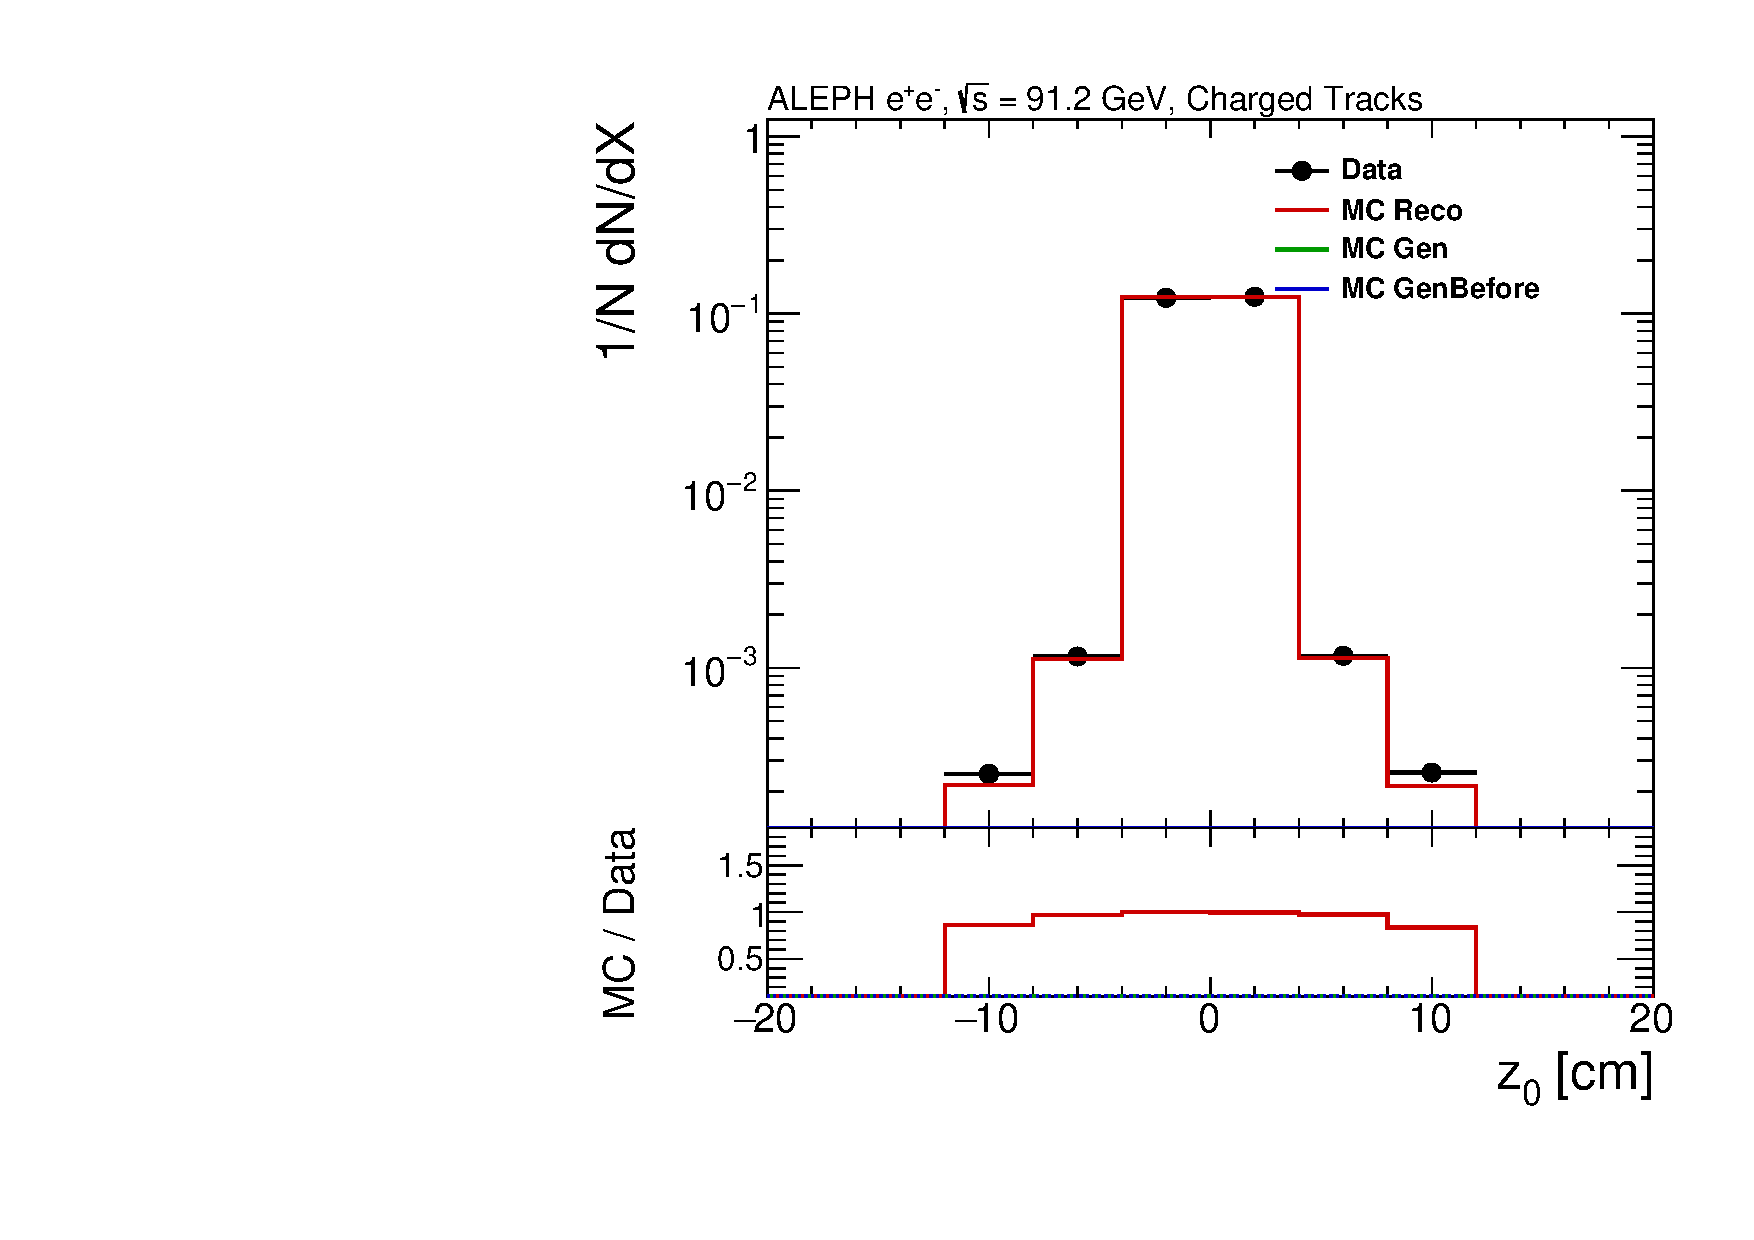
\includegraphics[width=0.325\textwidth]{../Studies/PreliminaryResult/2026-02-17_thrust_iter5/pwflag_kinematics/pwflag0_z0.pdf}
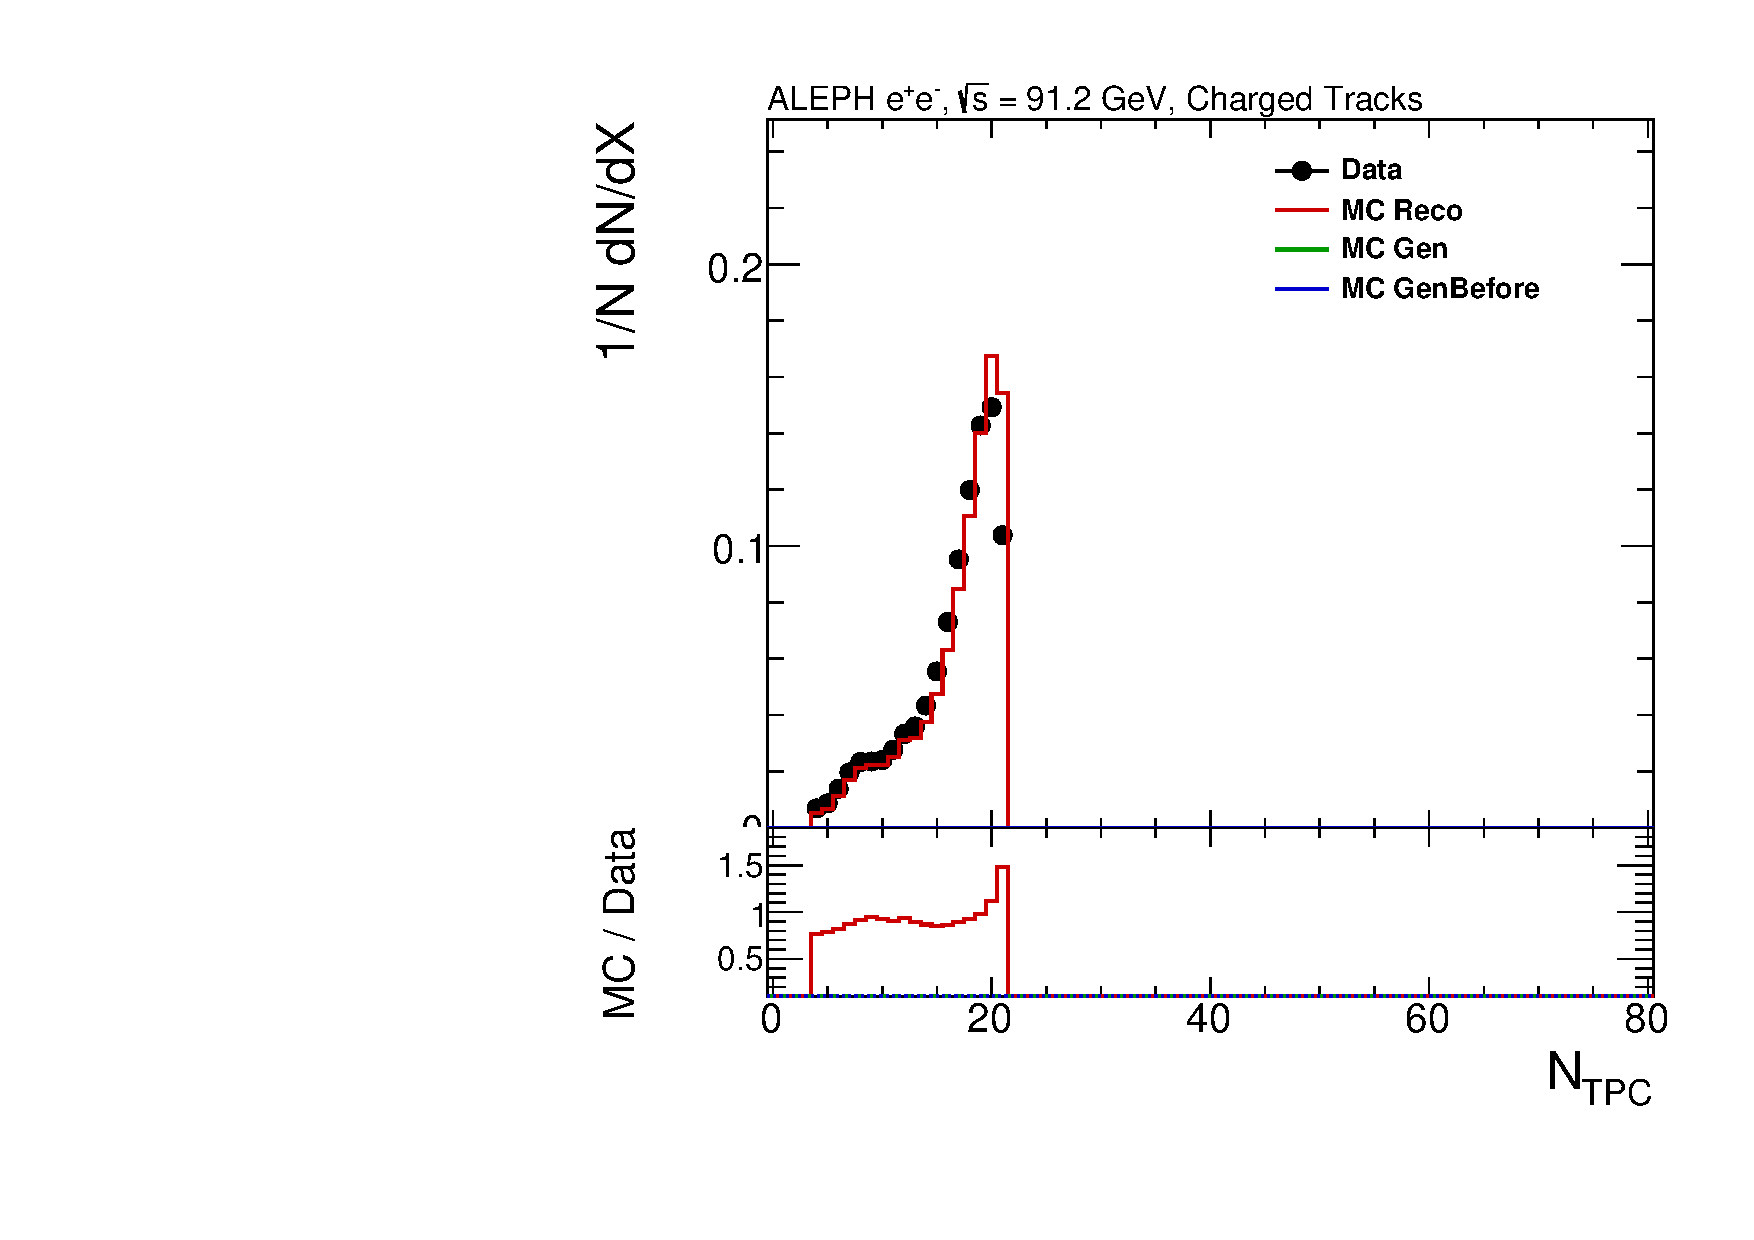
\includegraphics[width=0.325\textwidth]{../Studies/PreliminaryResult/2026-02-17_thrust_iter5/pwflag_kinematics/pwflag0_ntpc.pdf}
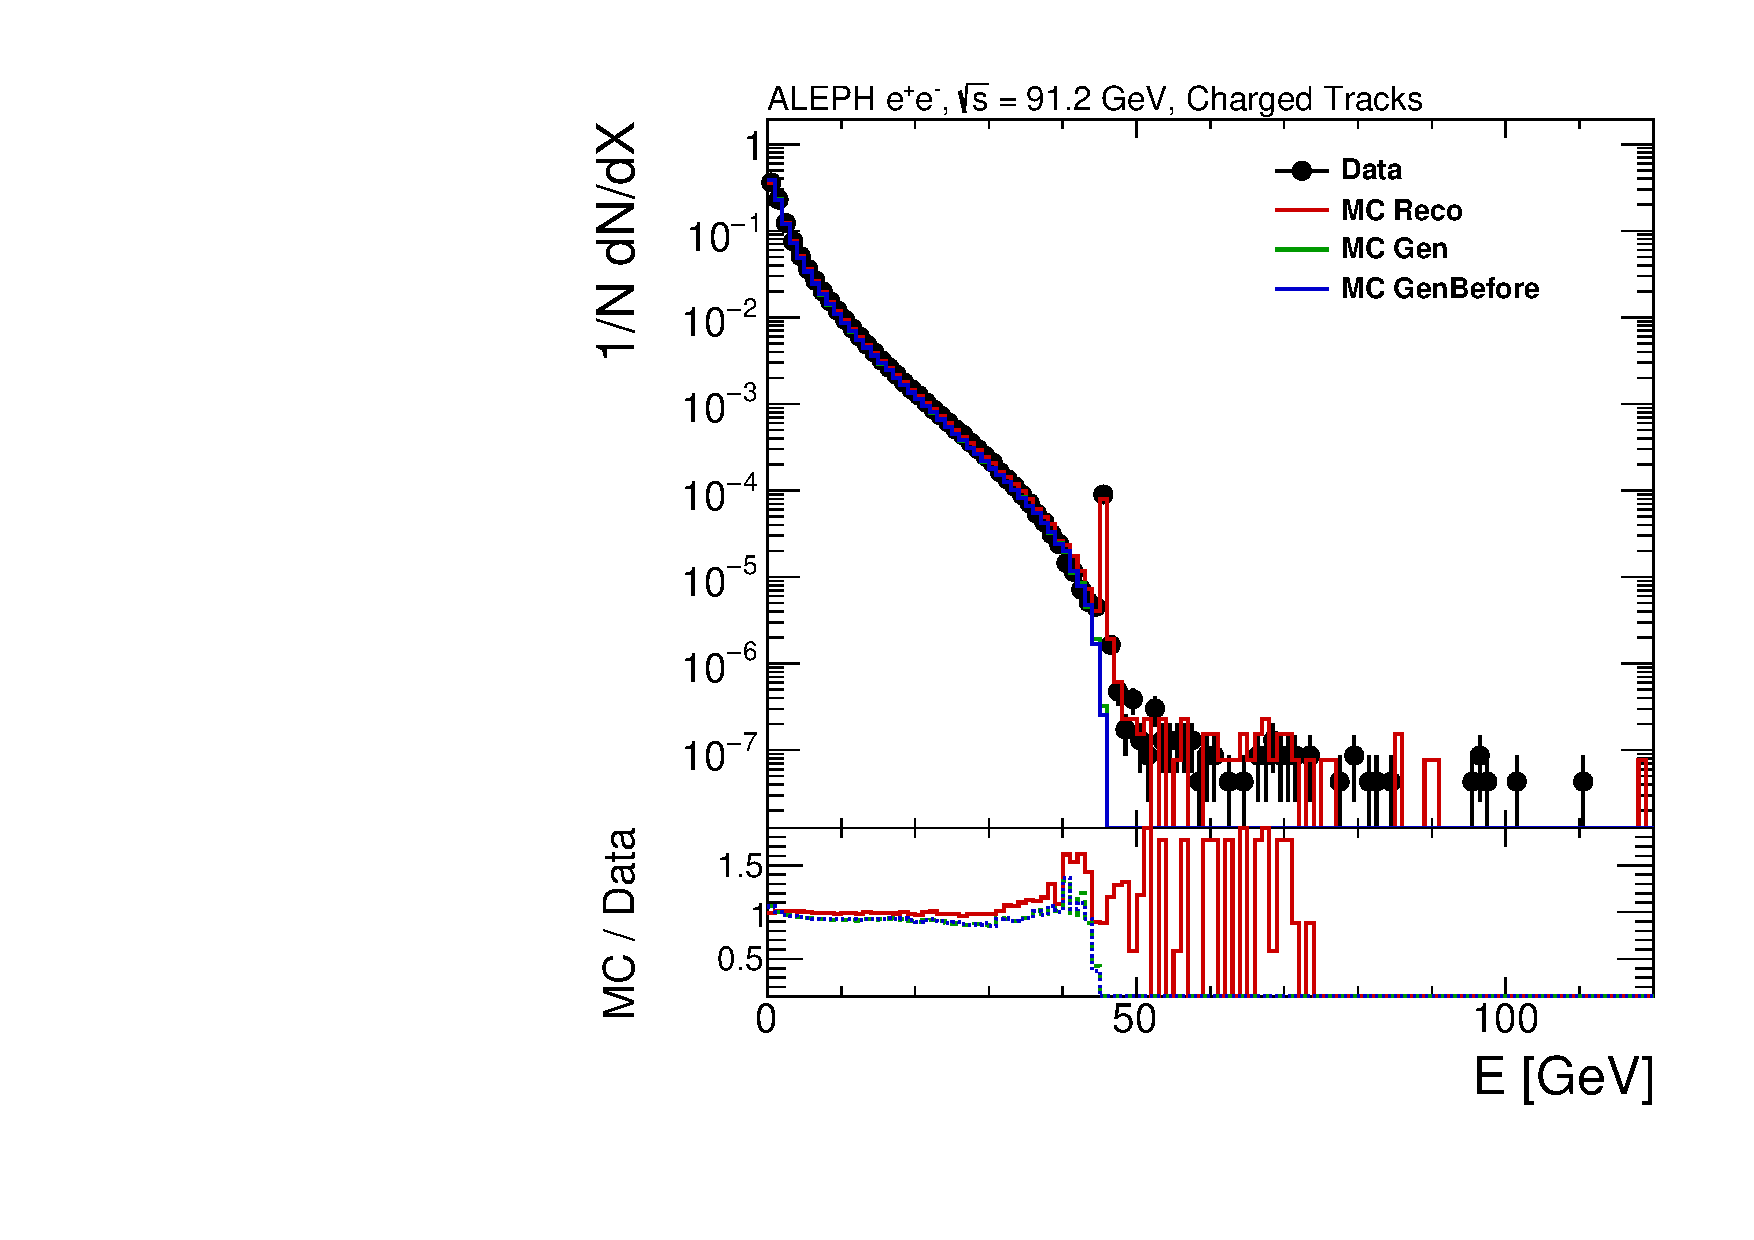
\includegraphics[width=0.325\textwidth]{../Studies/PreliminaryResult/2026-02-17_thrust_iter5/pwflag_kinematics/pwflag0_energy.pdf}
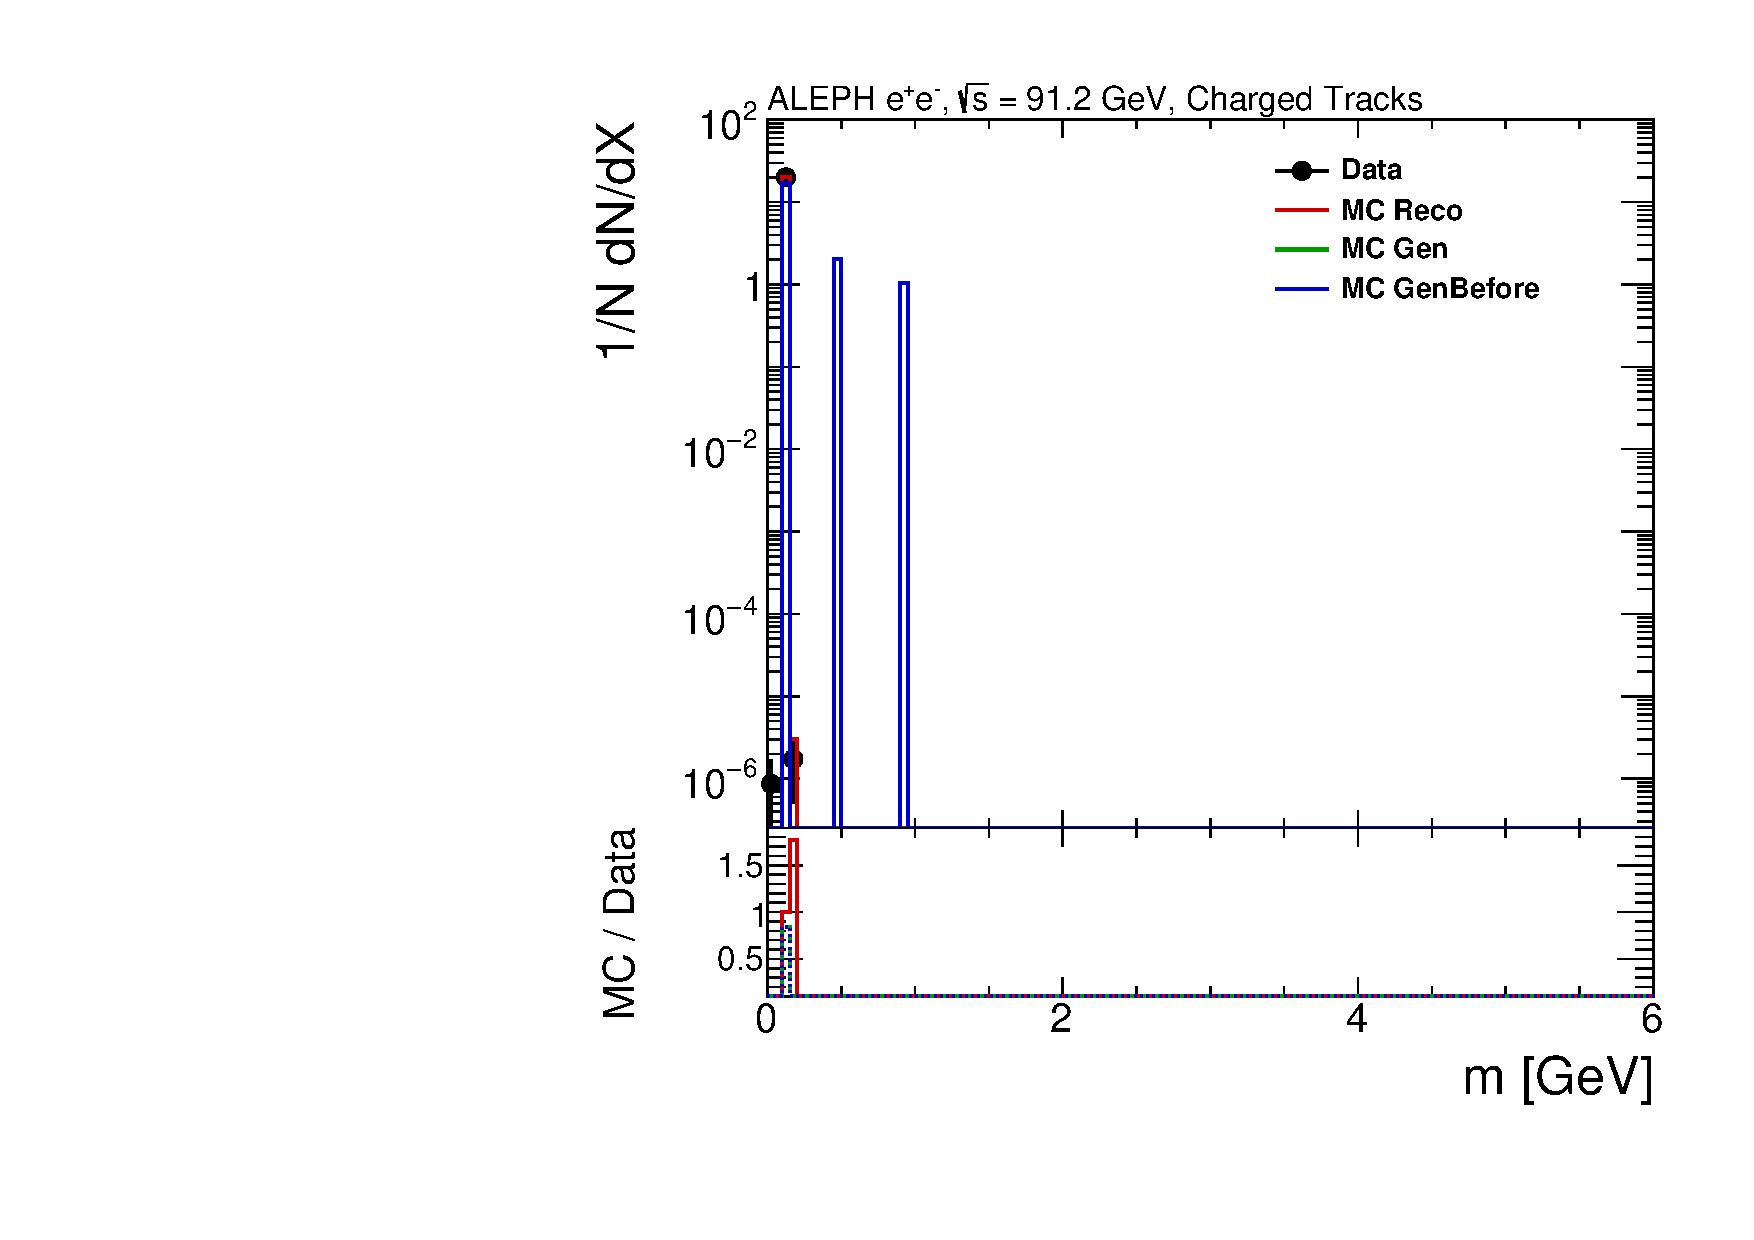
\includegraphics[width=0.325\textwidth]{../Studies/PreliminaryResult/2026-02-17_thrust_iter5/pwflag_kinematics/pwflag0_mass.pdf}
\caption{Complete \texttt{pwflag}=0 kinematic set.}
\label{fig:pwflag0_full}
\end{figure}

\noindent
In Fig.~\ref{fig:pwflag0_full}, the charged-track category drives the event-shape denominator
and axis finding, so agreement here anchors the full detector response modeling. The
$\cos\theta$ distribution shows the expected enhancement away from the acceptance edges and a
falloff near the fiducial boundary, while the $d_0$ and $z_0$ spectra are concentrated in the
high-quality track region selected for the nominal sample. The $N_{\mathrm{TPC}}$, $p_T$, and
energy panels provide direct checks that tracking-quality and hard-track tails are described with
the precision required for stable thrust unfolding.

\begin{figure}[t!]
\centering
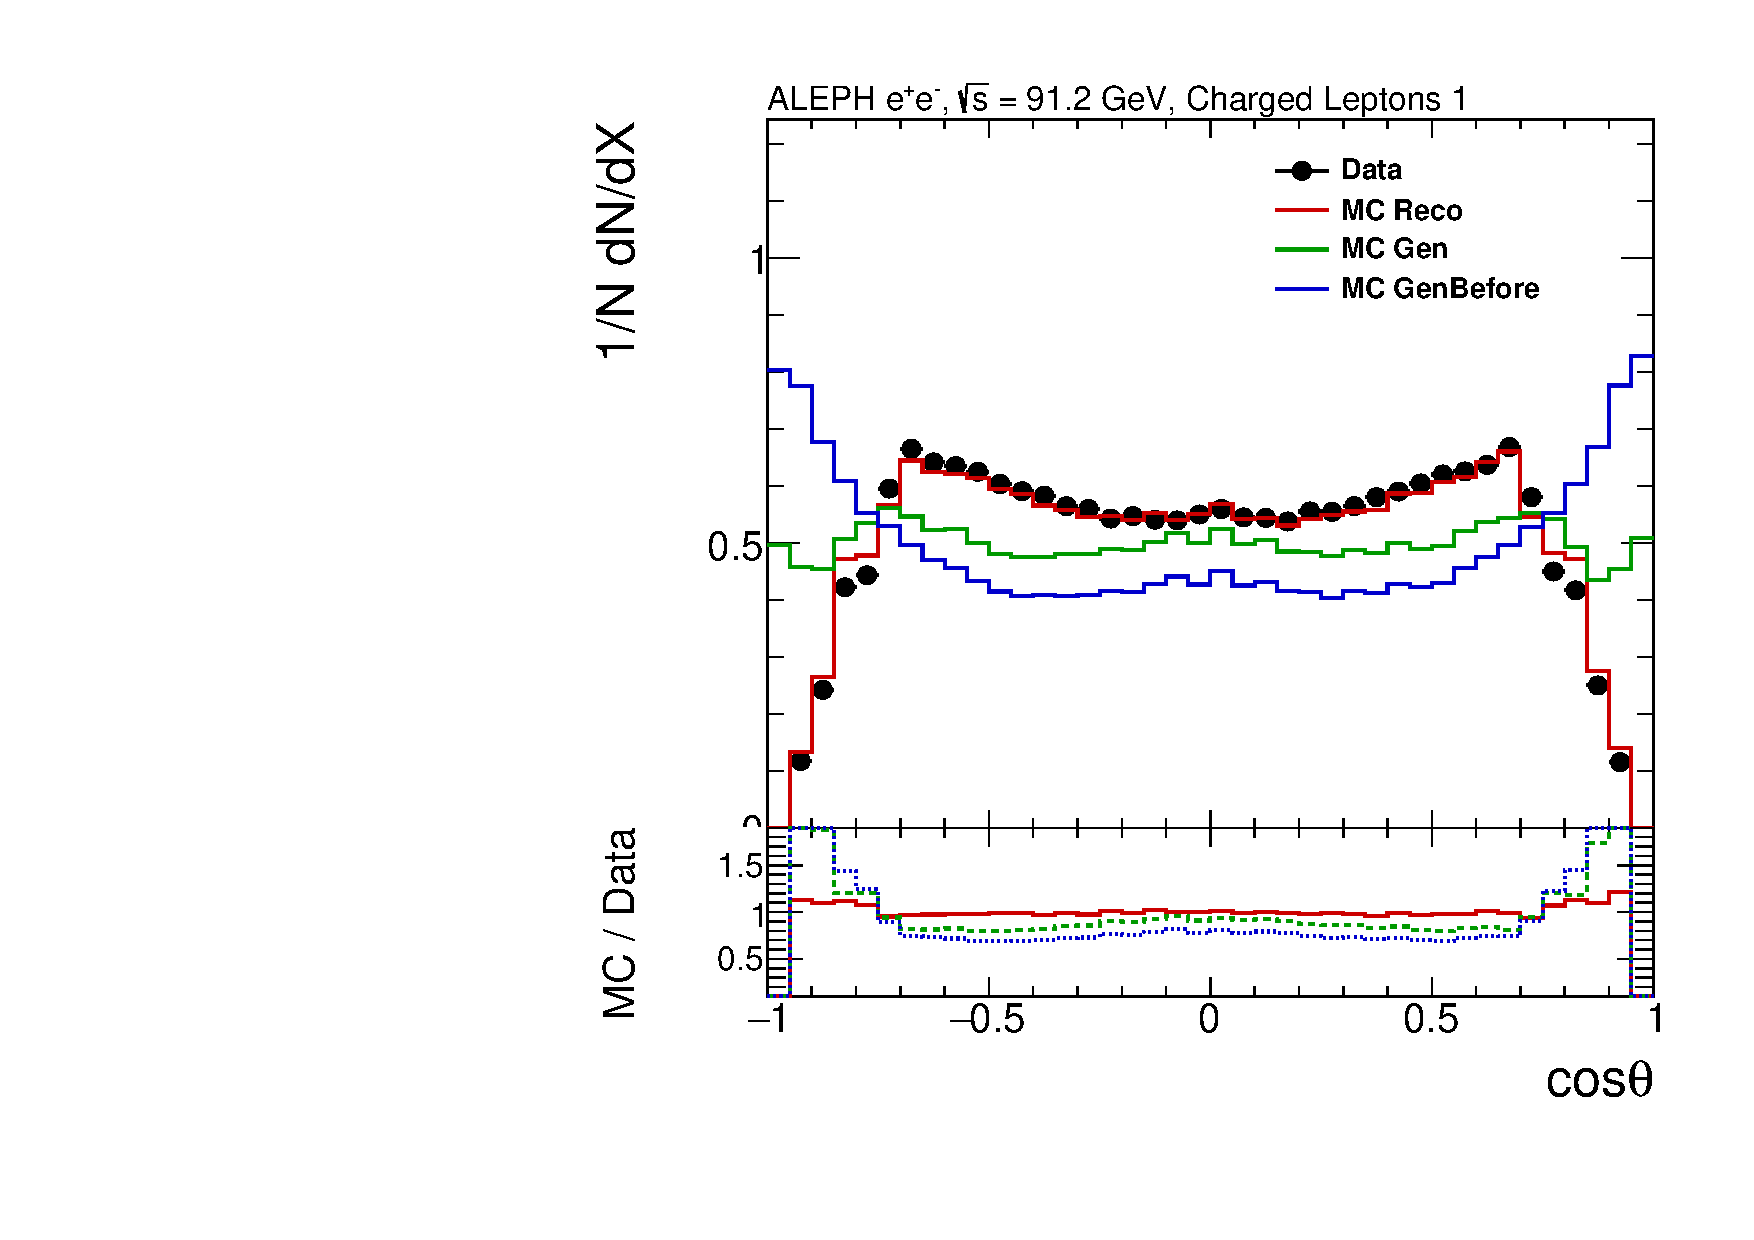
\includegraphics[width=0.325\textwidth]{../Studies/PreliminaryResult/2026-02-17_thrust_iter5/pwflag_kinematics/pwflag1_cosTheta.pdf}
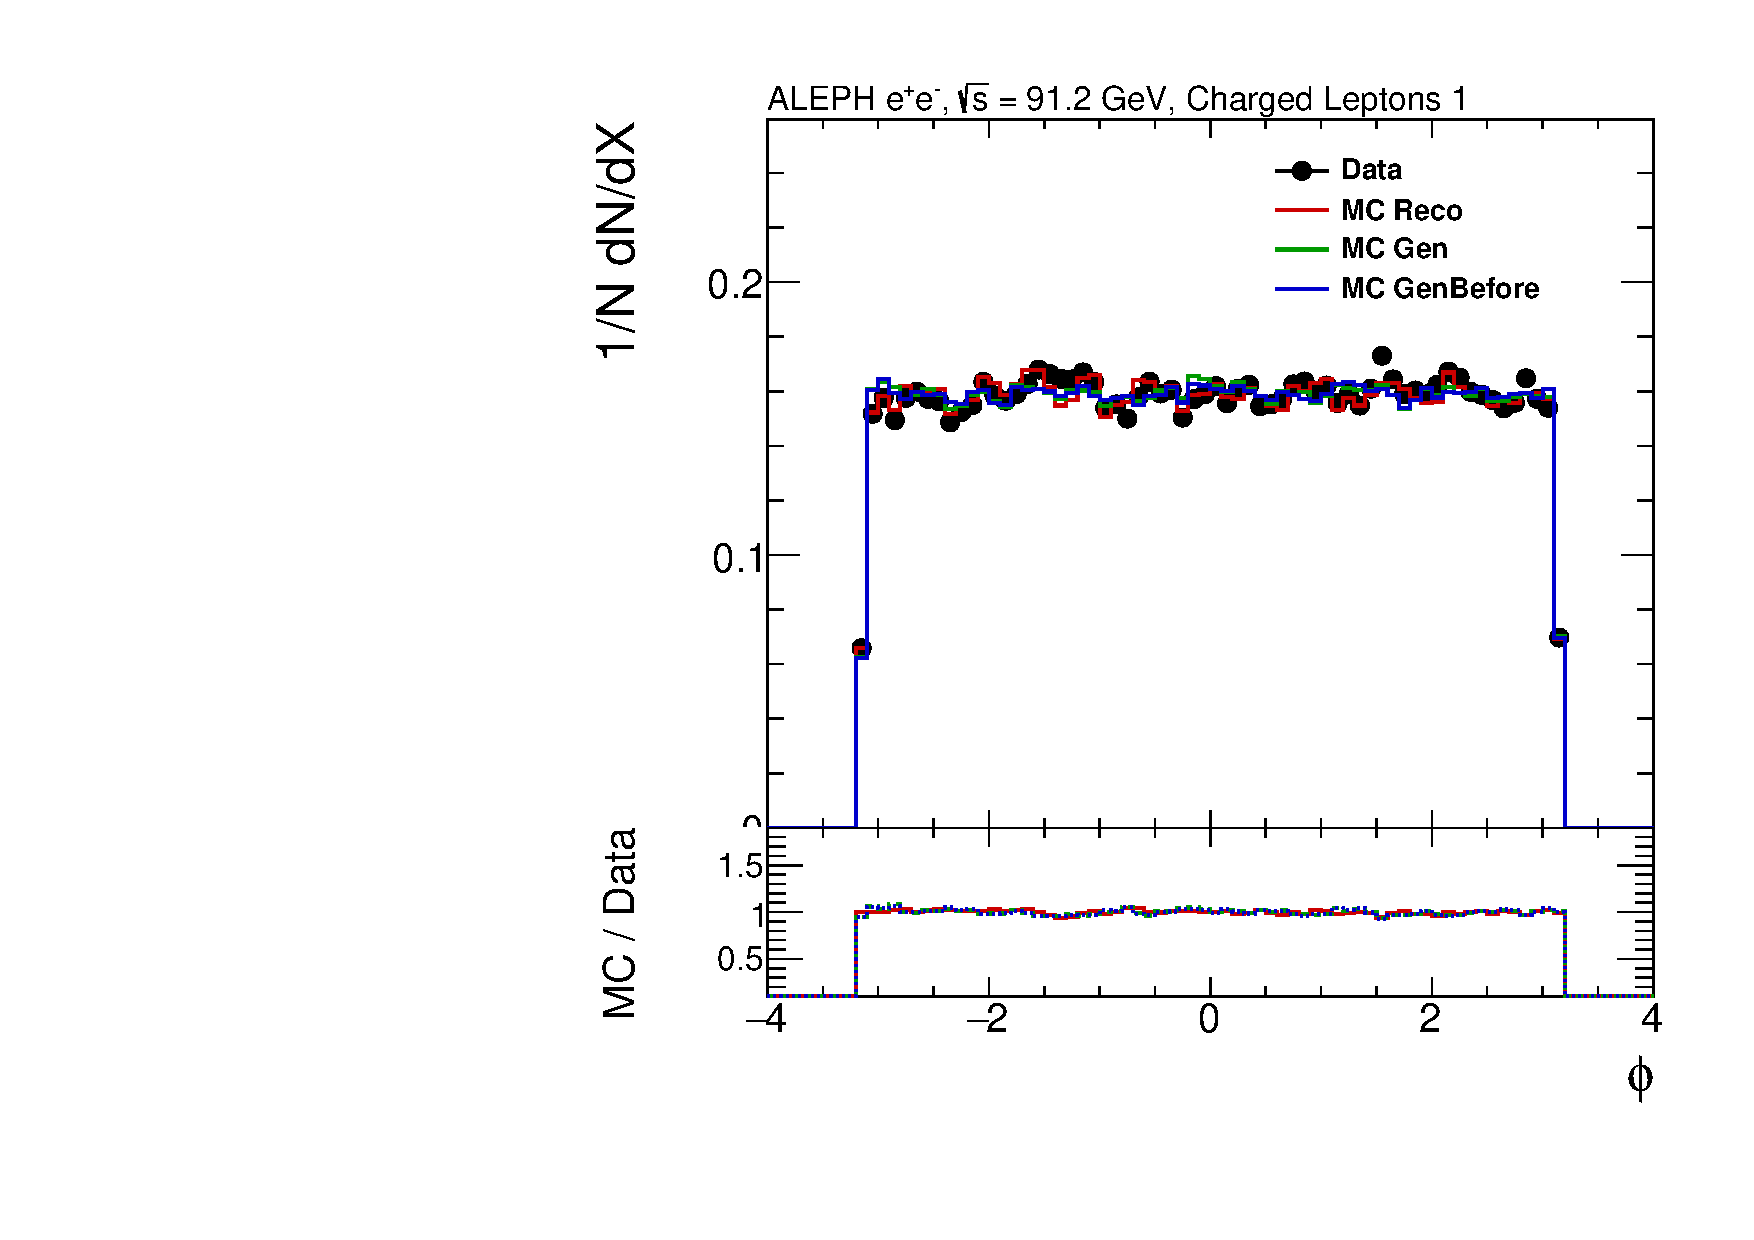
\includegraphics[width=0.325\textwidth]{../Studies/PreliminaryResult/2026-02-17_thrust_iter5/pwflag_kinematics/pwflag1_phi.pdf}
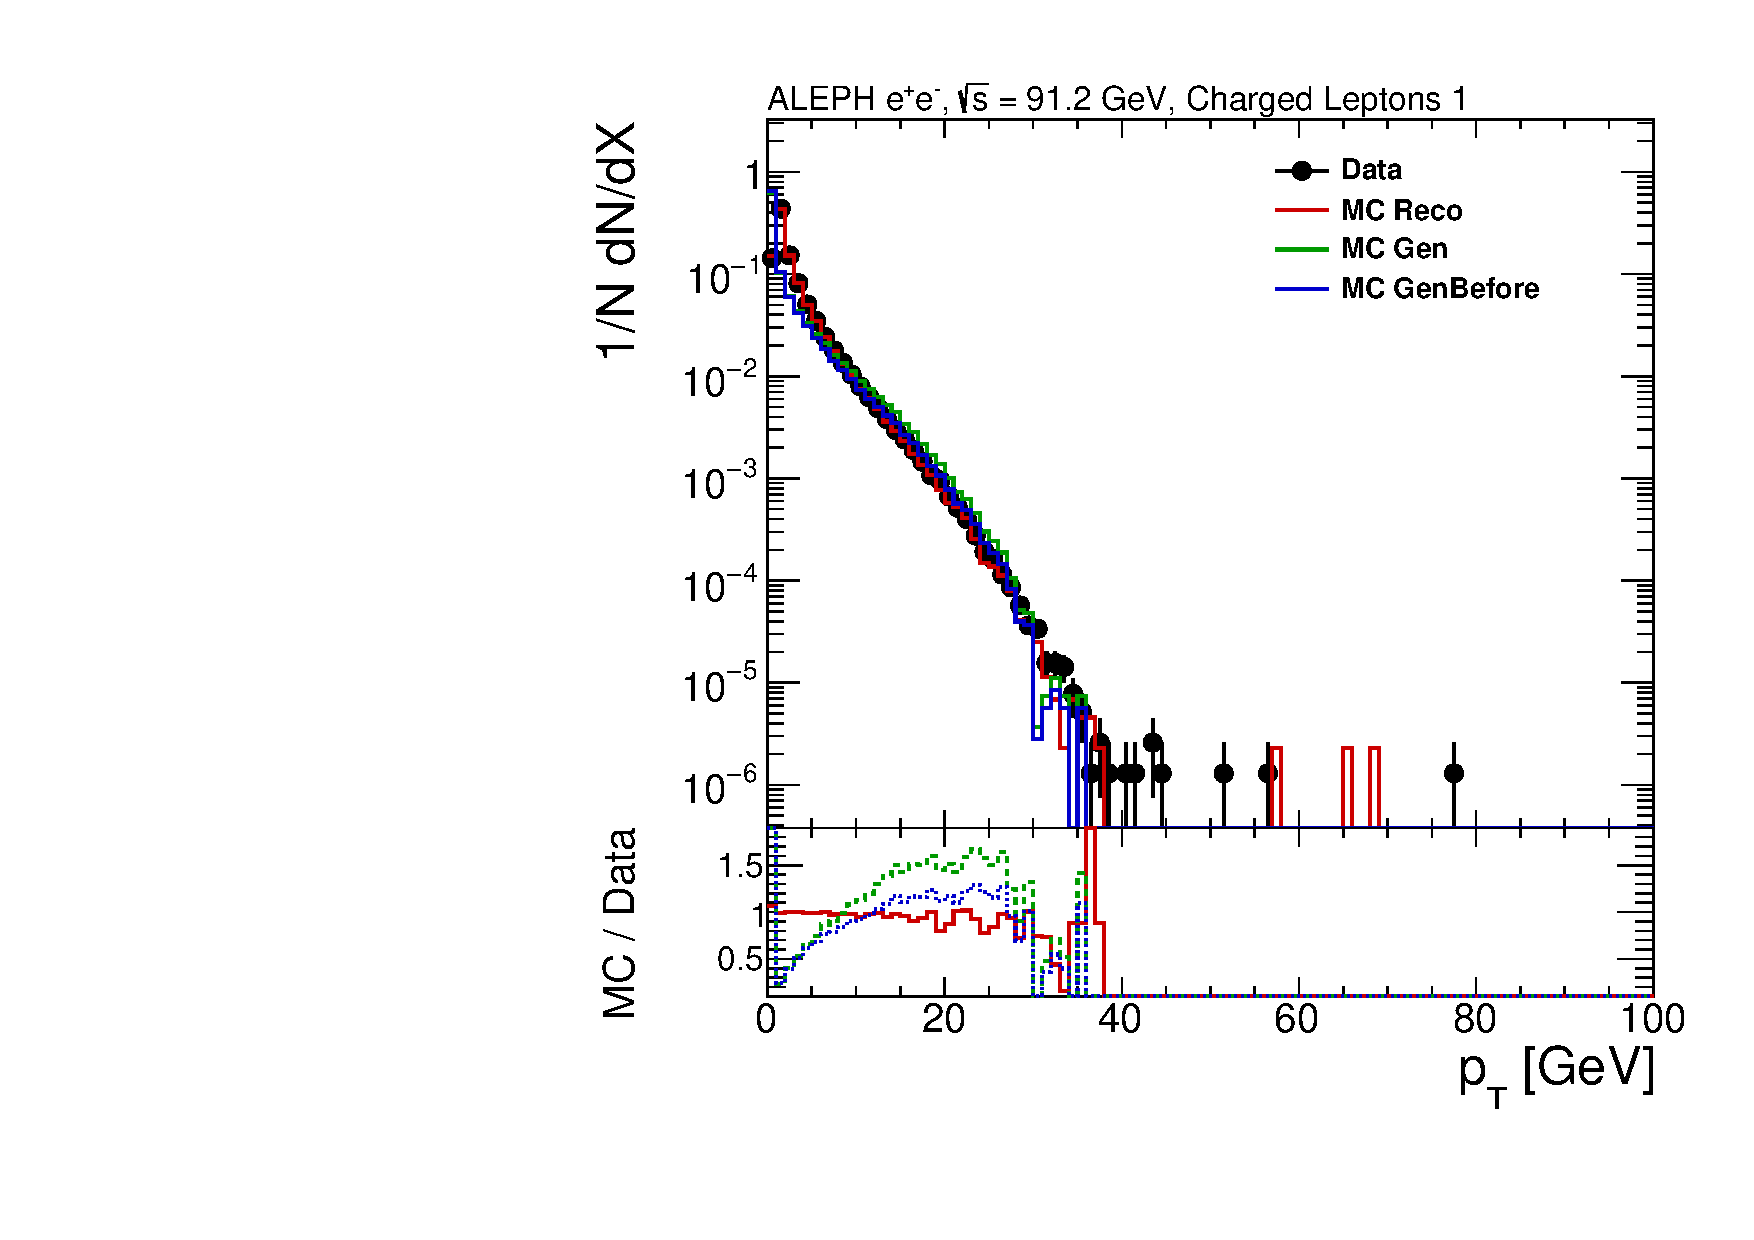
\includegraphics[width=0.325\textwidth]{../Studies/PreliminaryResult/2026-02-17_thrust_iter5/pwflag_kinematics/pwflag1_pt.pdf}
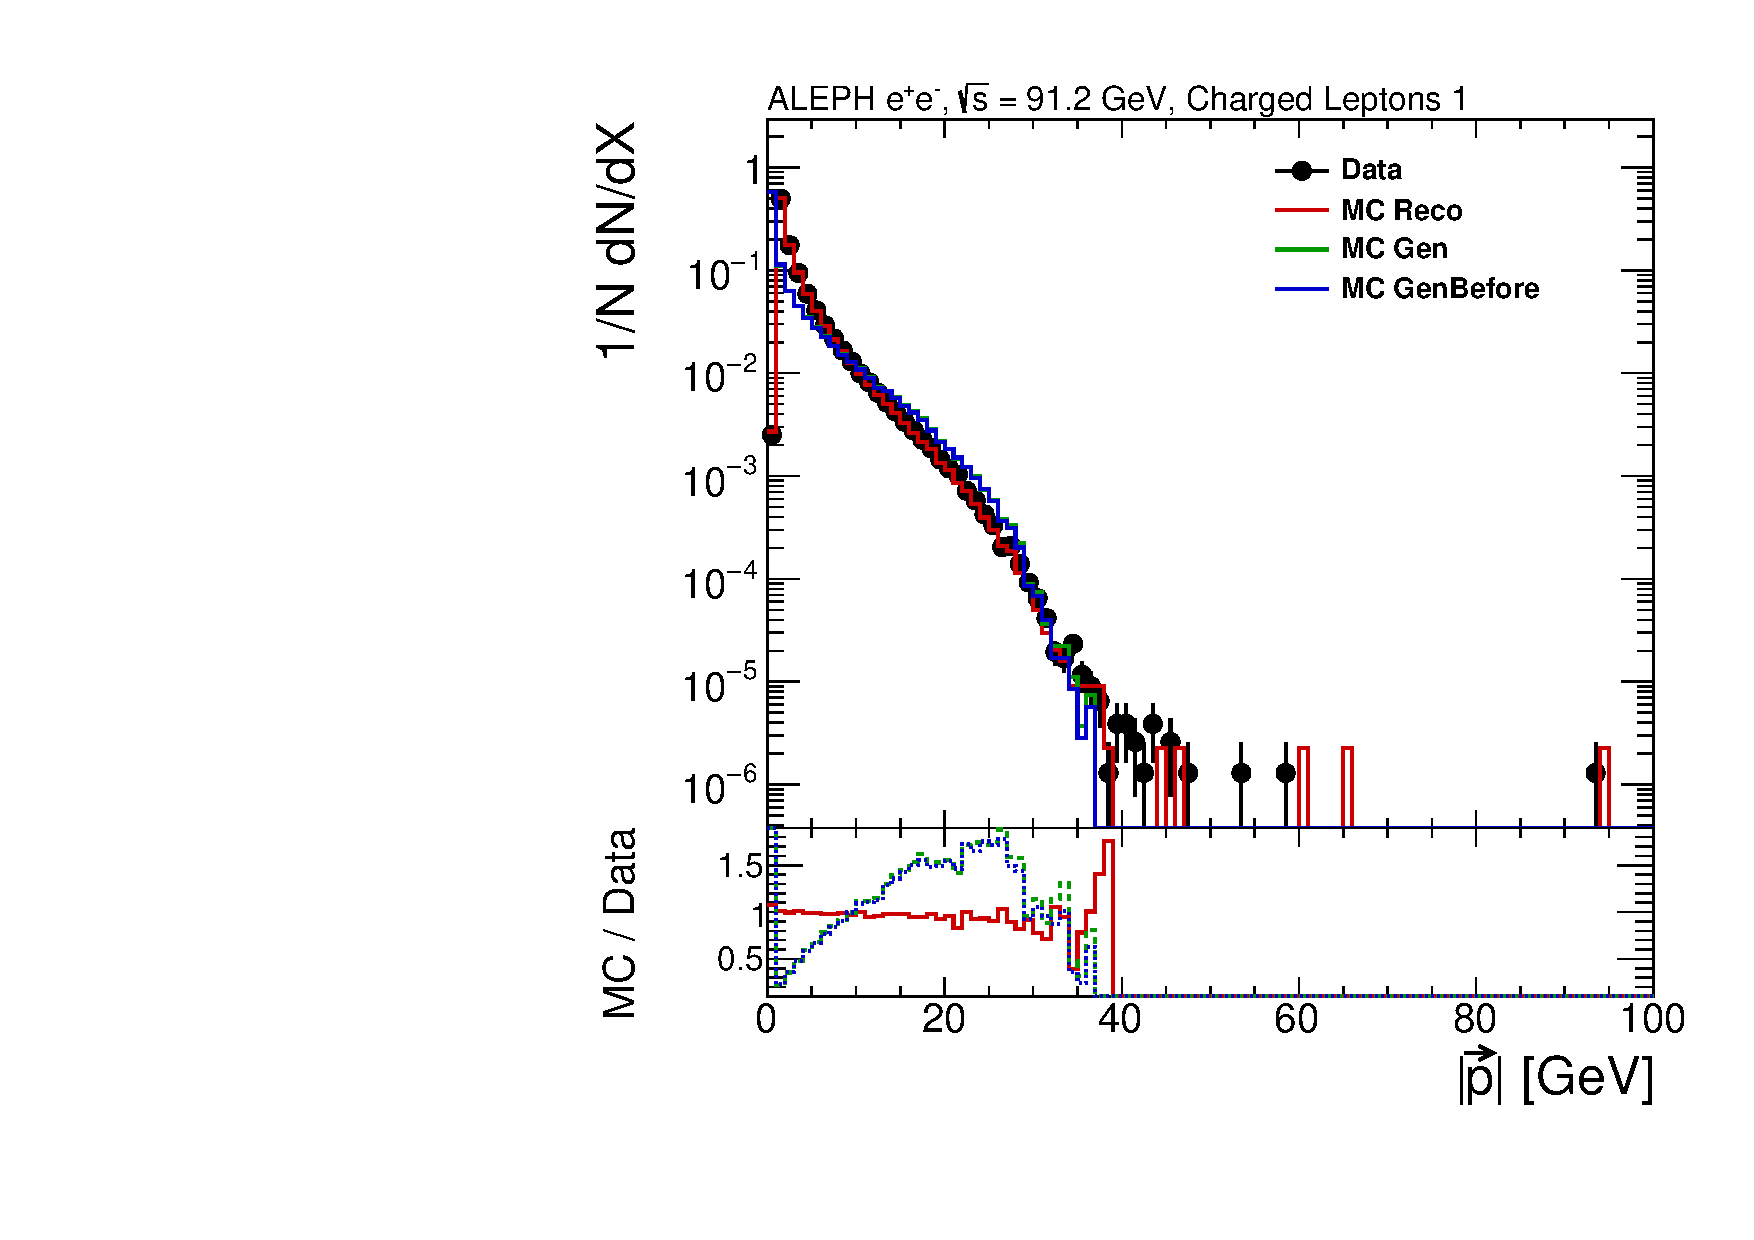
\includegraphics[width=0.325\textwidth]{../Studies/PreliminaryResult/2026-02-17_thrust_iter5/pwflag_kinematics/pwflag1_pmag.pdf}
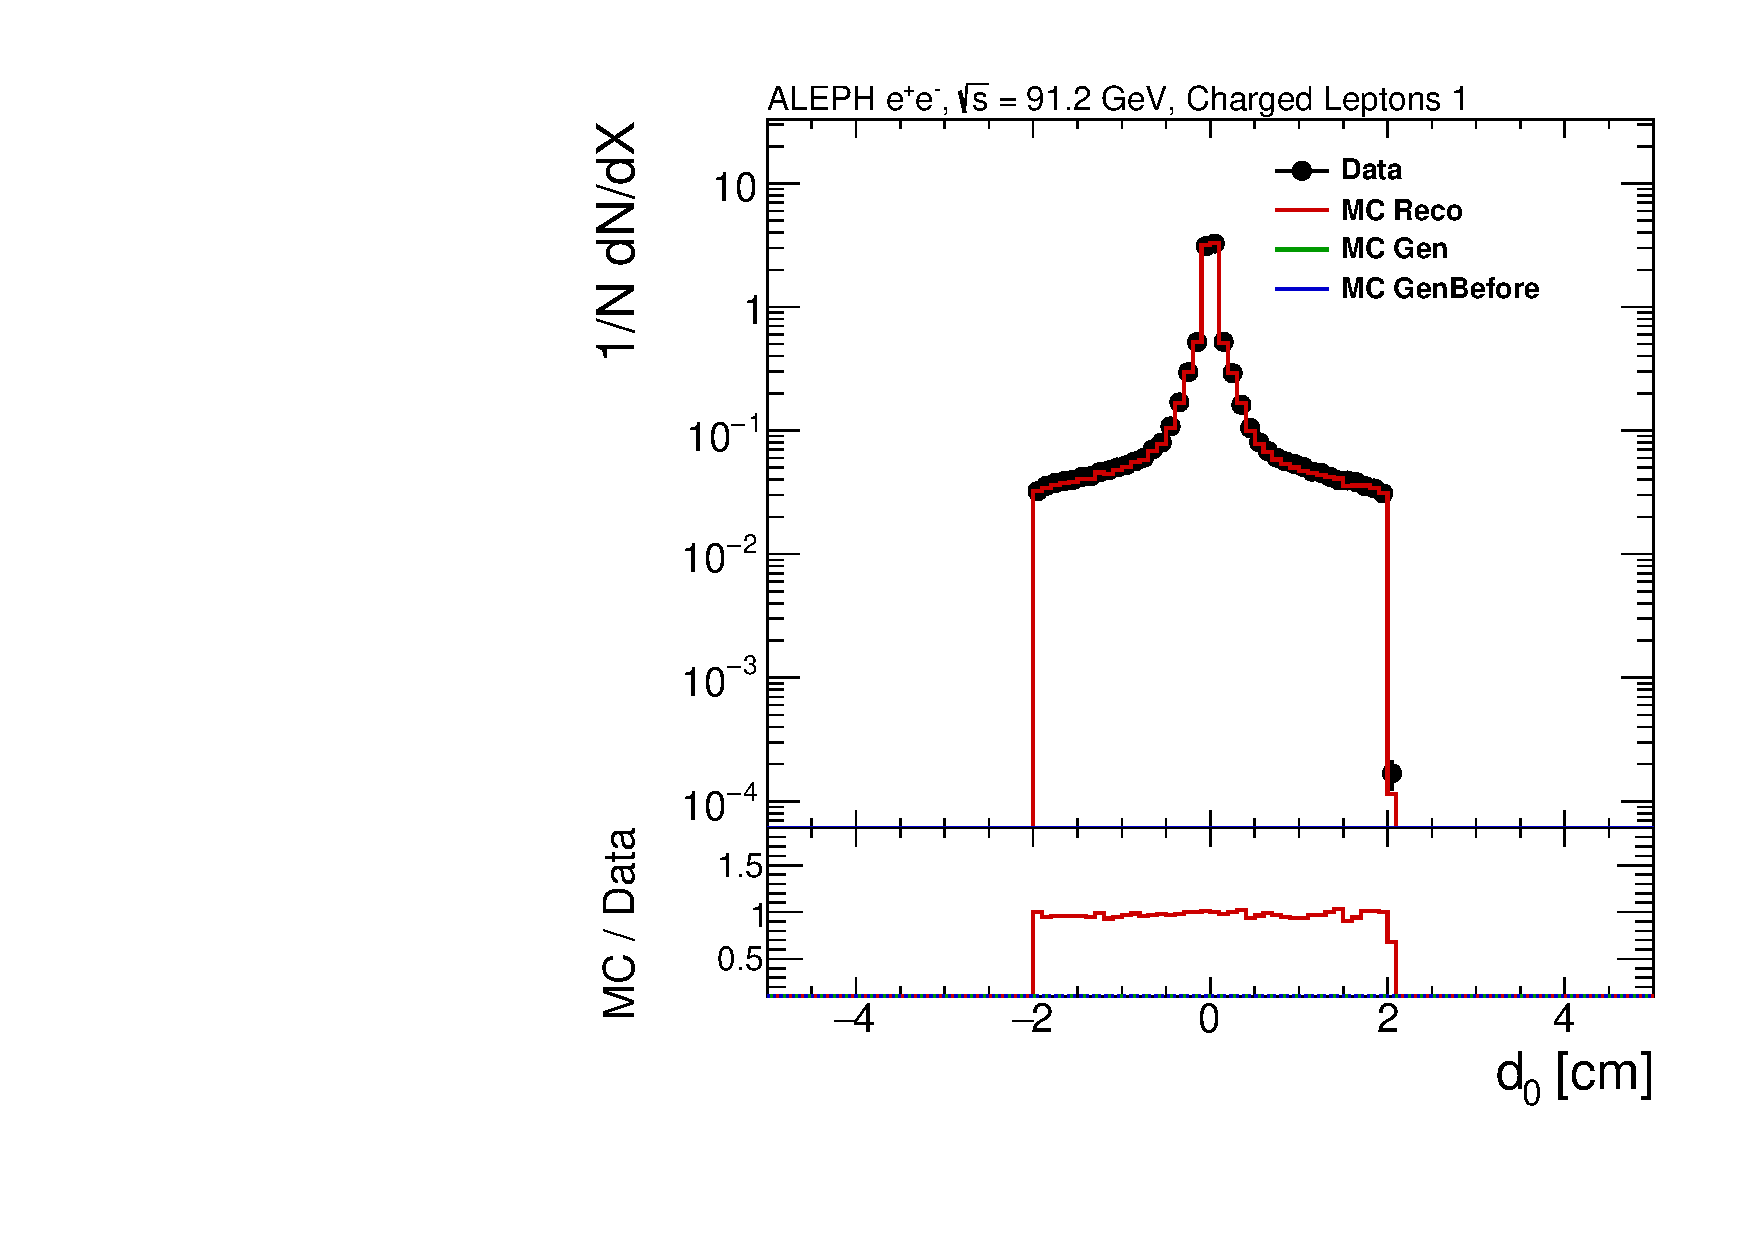
\includegraphics[width=0.325\textwidth]{../Studies/PreliminaryResult/2026-02-17_thrust_iter5/pwflag_kinematics/pwflag1_d0.pdf}
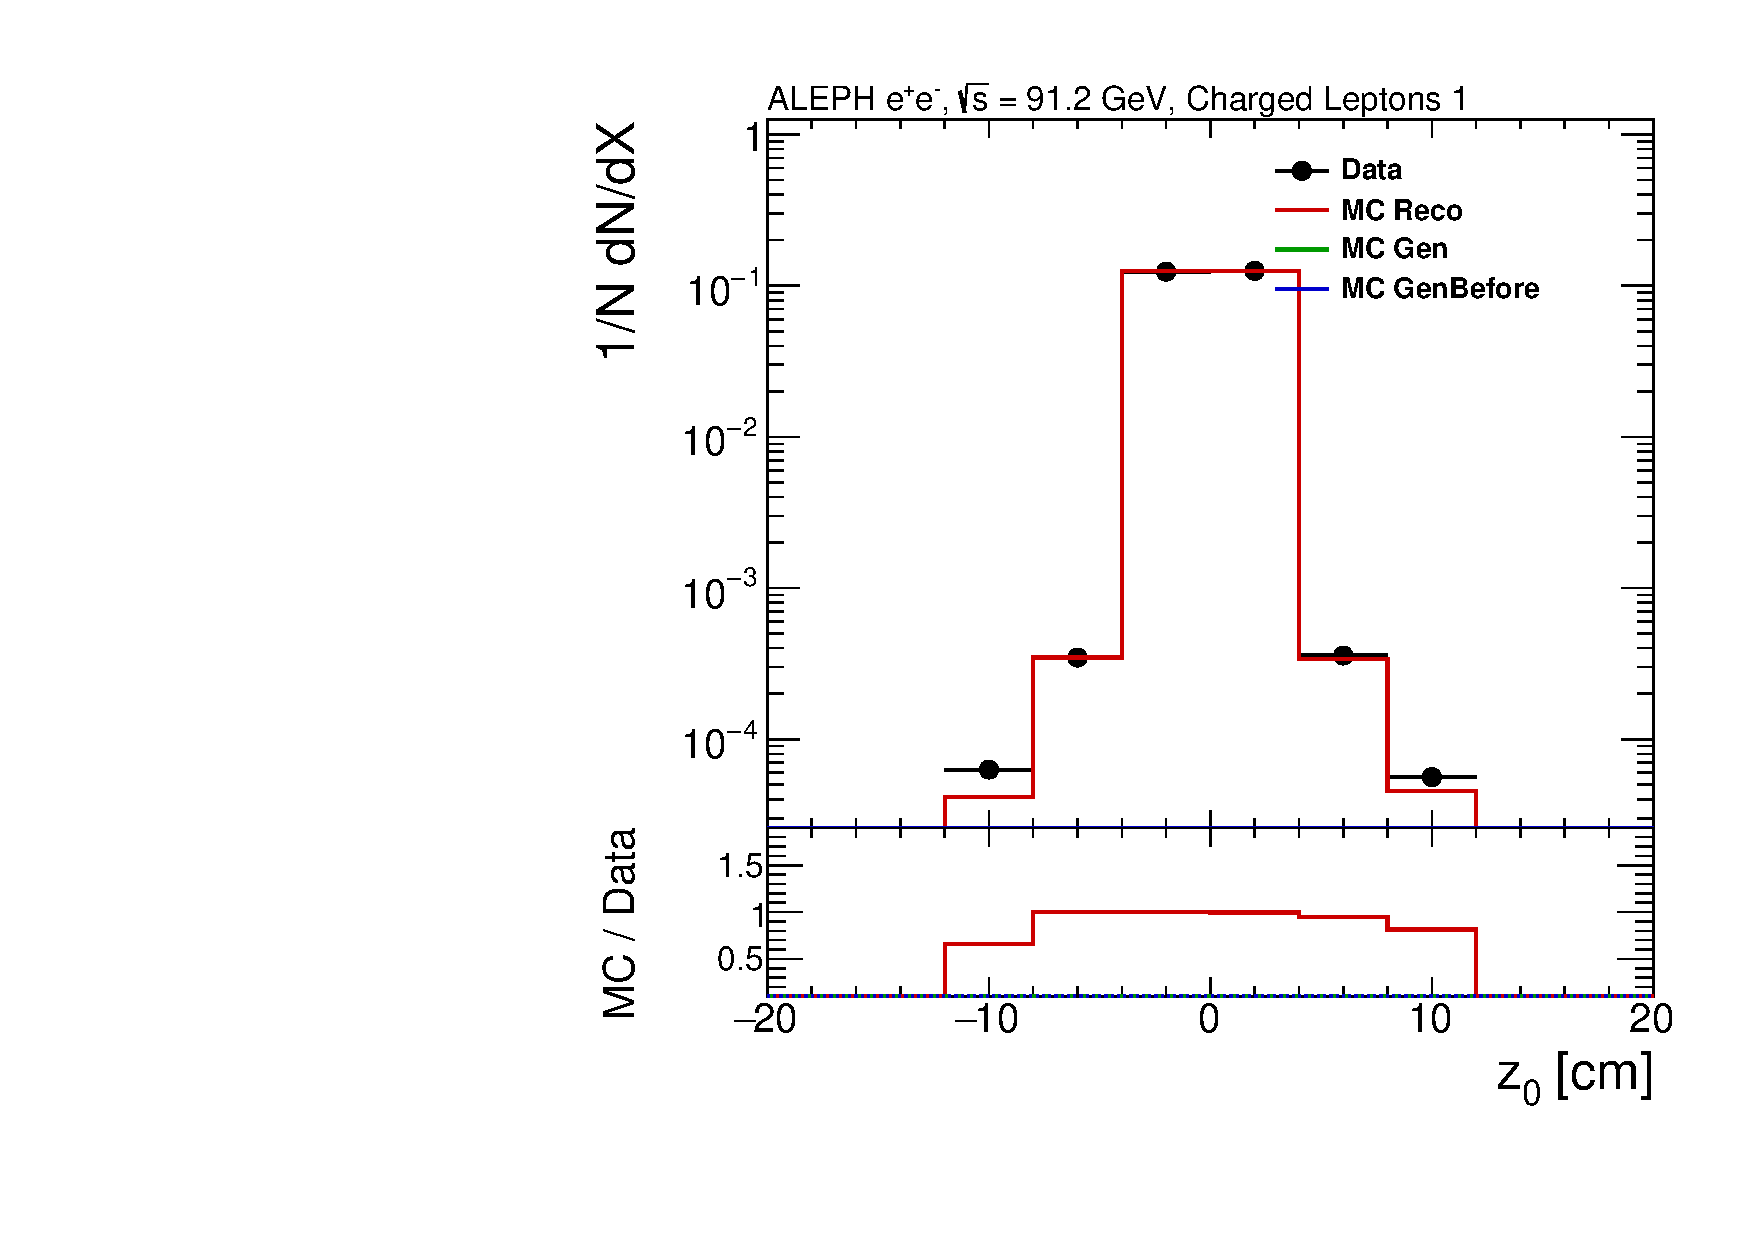
\includegraphics[width=0.325\textwidth]{../Studies/PreliminaryResult/2026-02-17_thrust_iter5/pwflag_kinematics/pwflag1_z0.pdf}
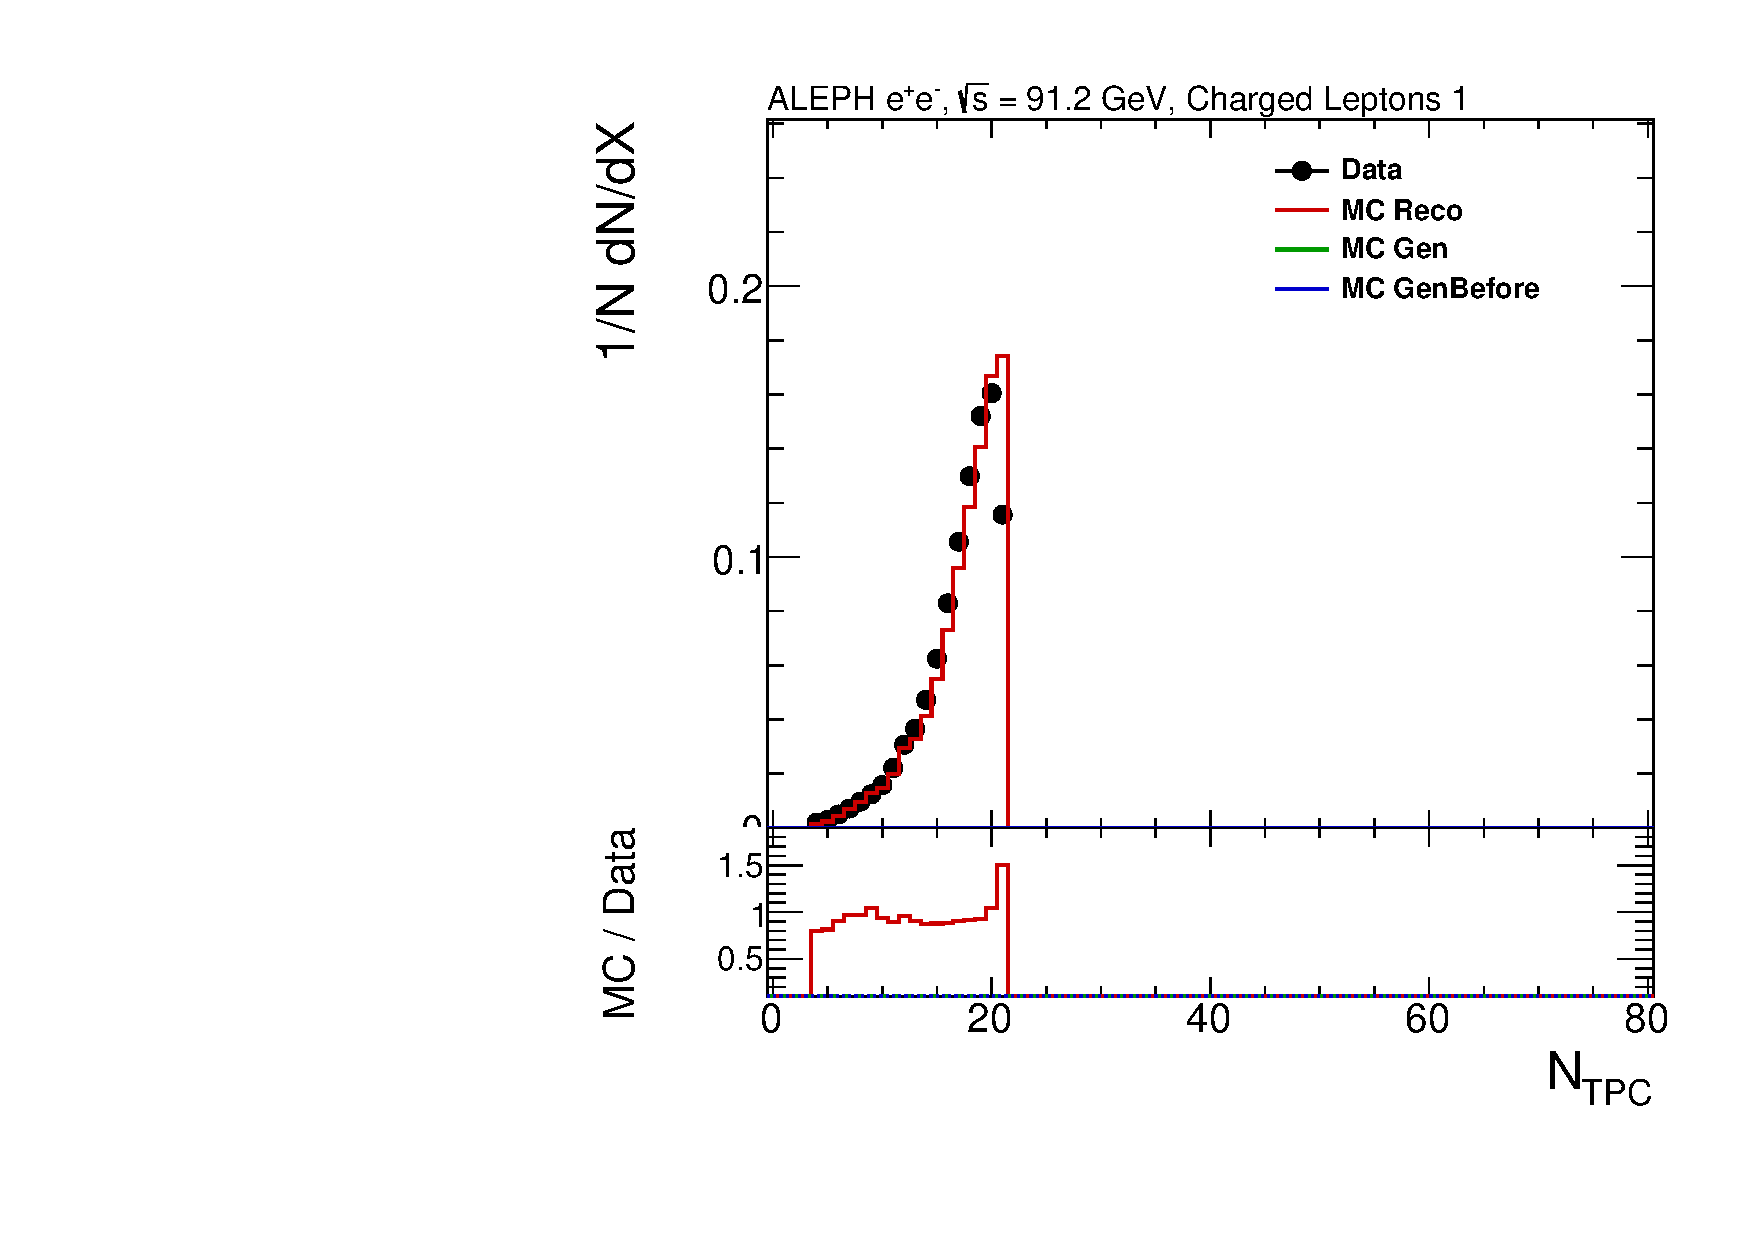
\includegraphics[width=0.325\textwidth]{../Studies/PreliminaryResult/2026-02-17_thrust_iter5/pwflag_kinematics/pwflag1_ntpc.pdf}
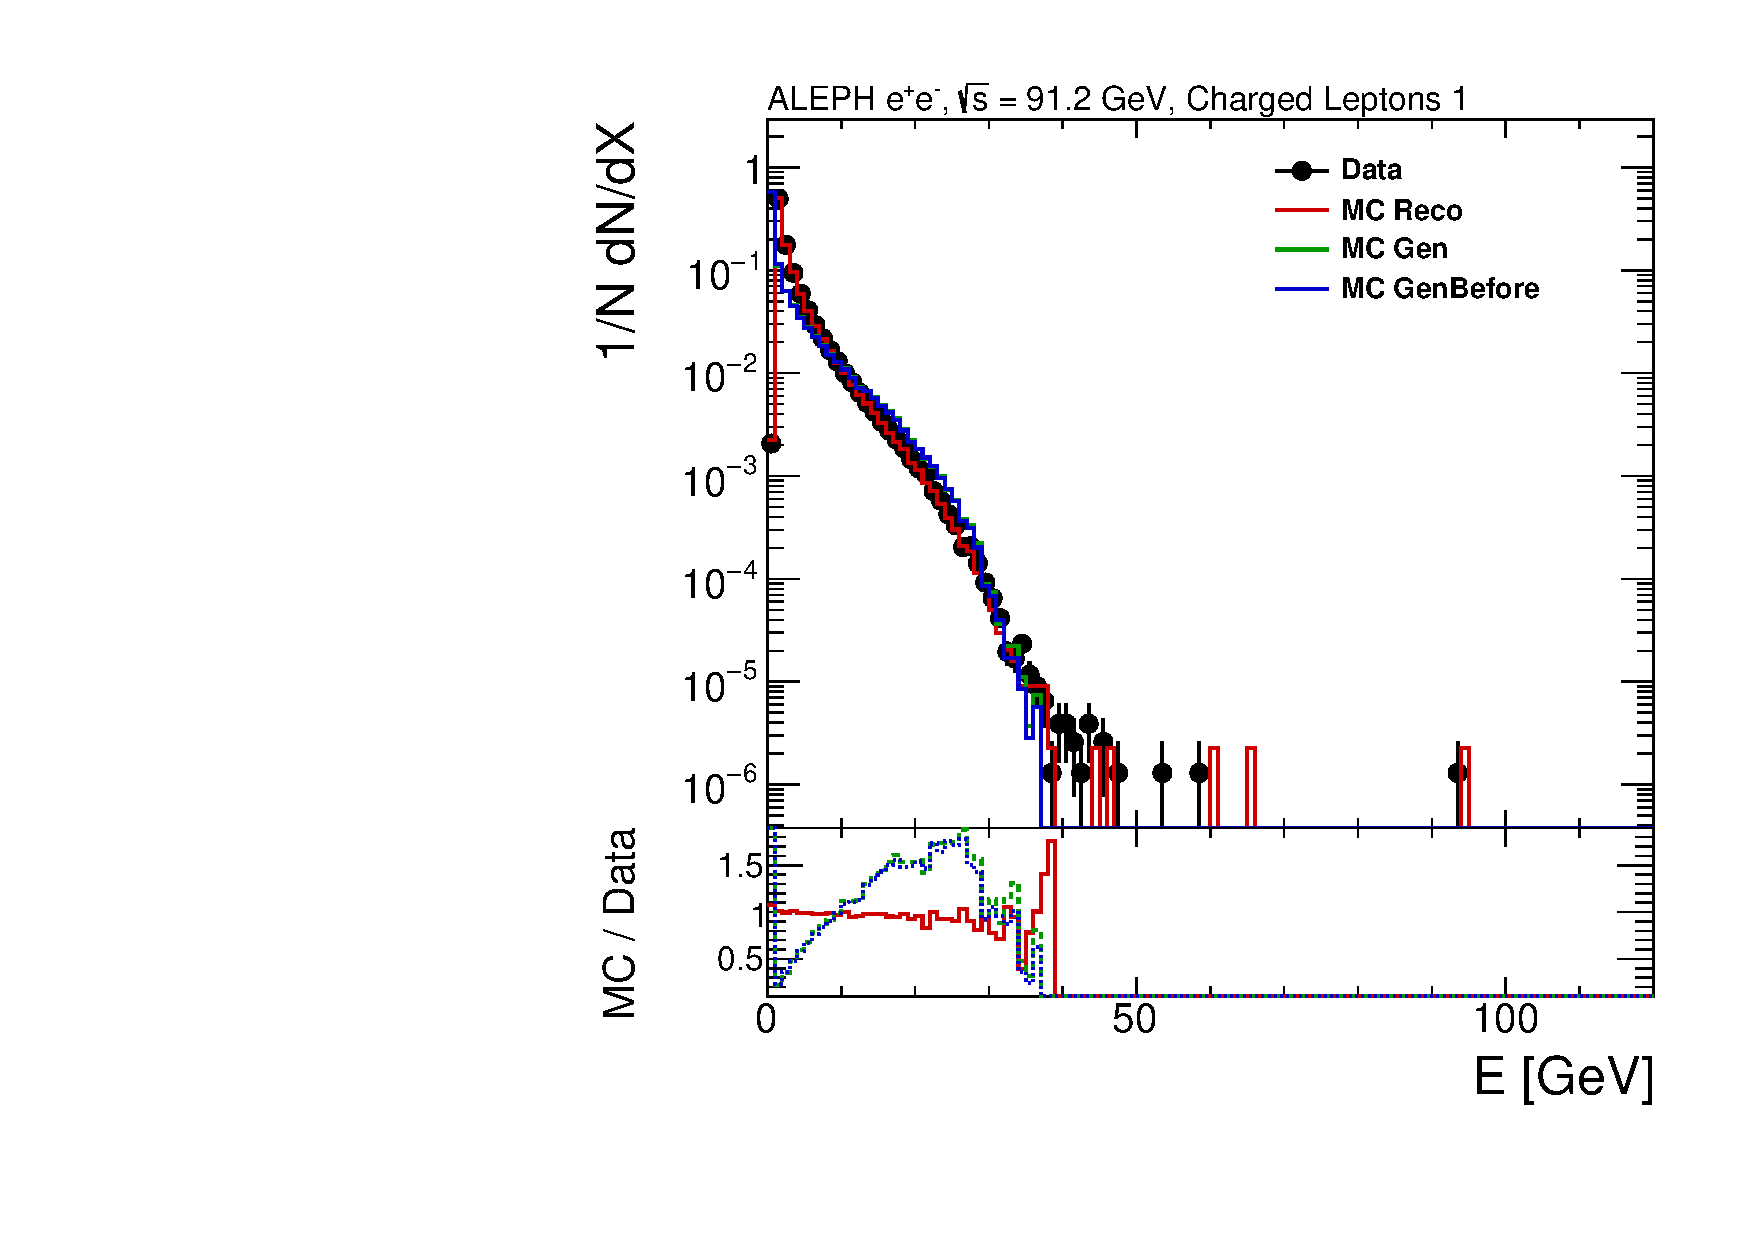
\includegraphics[width=0.325\textwidth]{../Studies/PreliminaryResult/2026-02-17_thrust_iter5/pwflag_kinematics/pwflag1_energy.pdf}
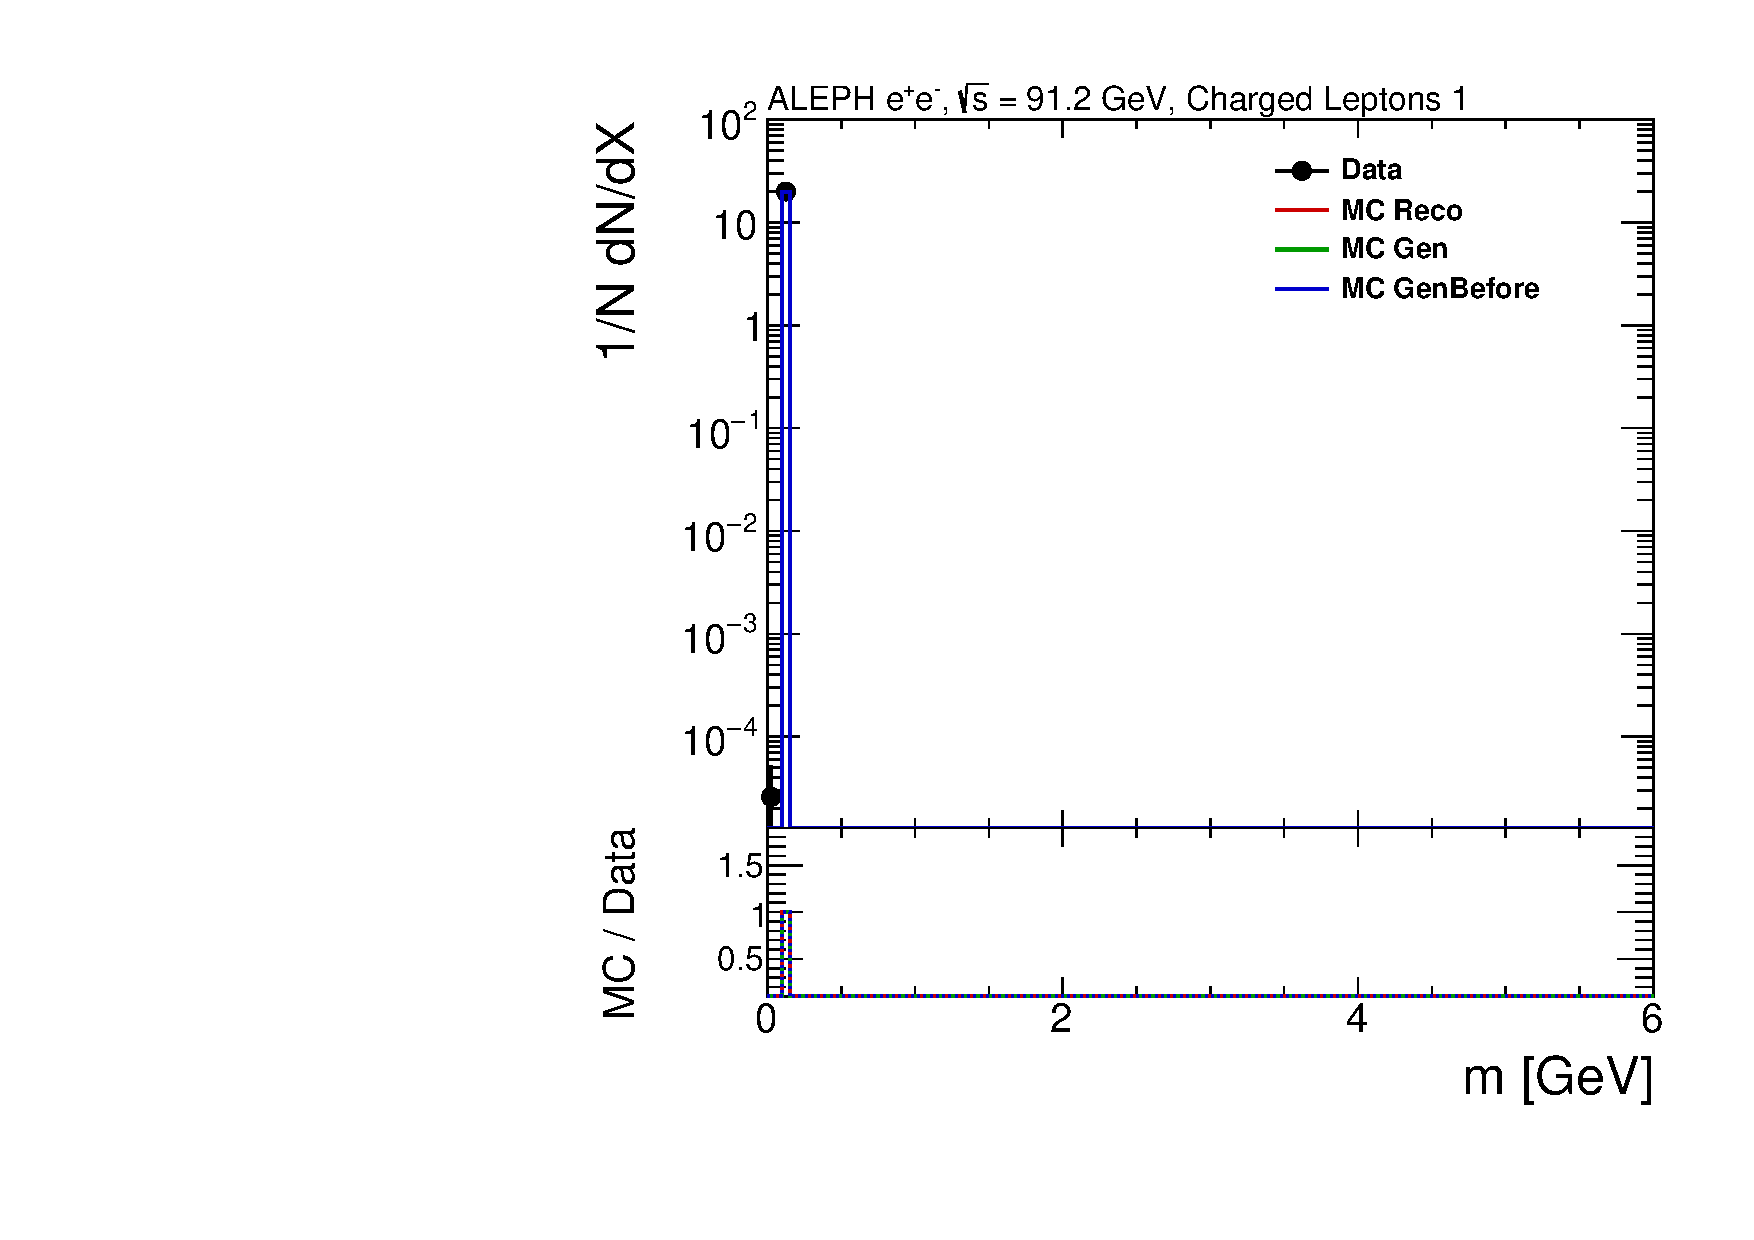
\includegraphics[width=0.325\textwidth]{../Studies/PreliminaryResult/2026-02-17_thrust_iter5/pwflag_kinematics/pwflag1_mass.pdf}
\caption{Complete \texttt{pwflag}=1 kinematic set.}
\label{fig:pwflag1_full}
\end{figure}

\noindent
Figure~\ref{fig:pwflag1_full} shows the first charged-lepton class used in the nominal object
list; these lower-rate objects still affect event axes in asymmetric topologies. Relative to
charged tracks, this category has smaller yields and larger statistical fluctuations, but the
detector-level and MC shapes remain consistent across the main selection observables. The
comparison is important because isolated energetic leptons can rotate the thrust axis in otherwise
two-jet-like events and can therefore influence migration in specific bins.

\begin{figure}[t!]
\centering
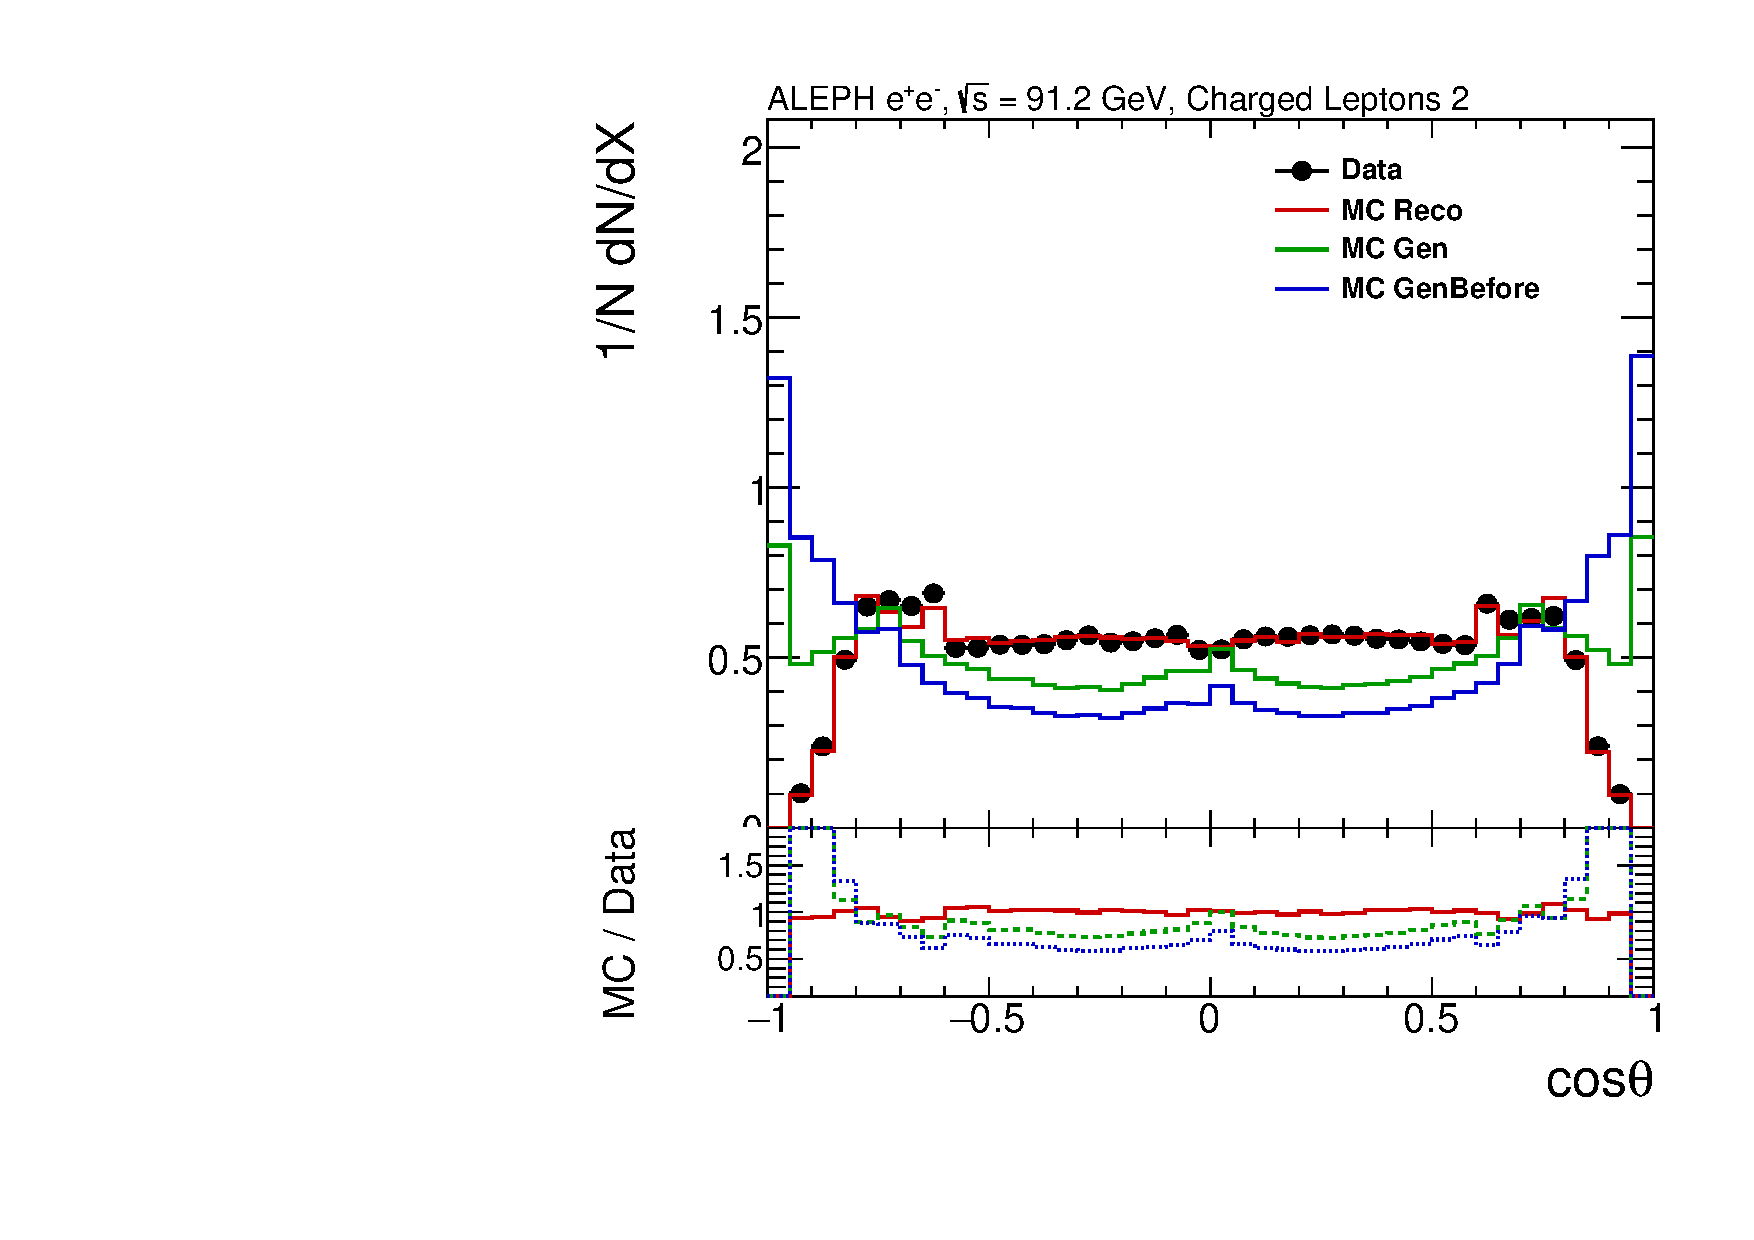
\includegraphics[width=0.325\textwidth]{../Studies/PreliminaryResult/2026-02-17_thrust_iter5/pwflag_kinematics/pwflag2_cosTheta.pdf}
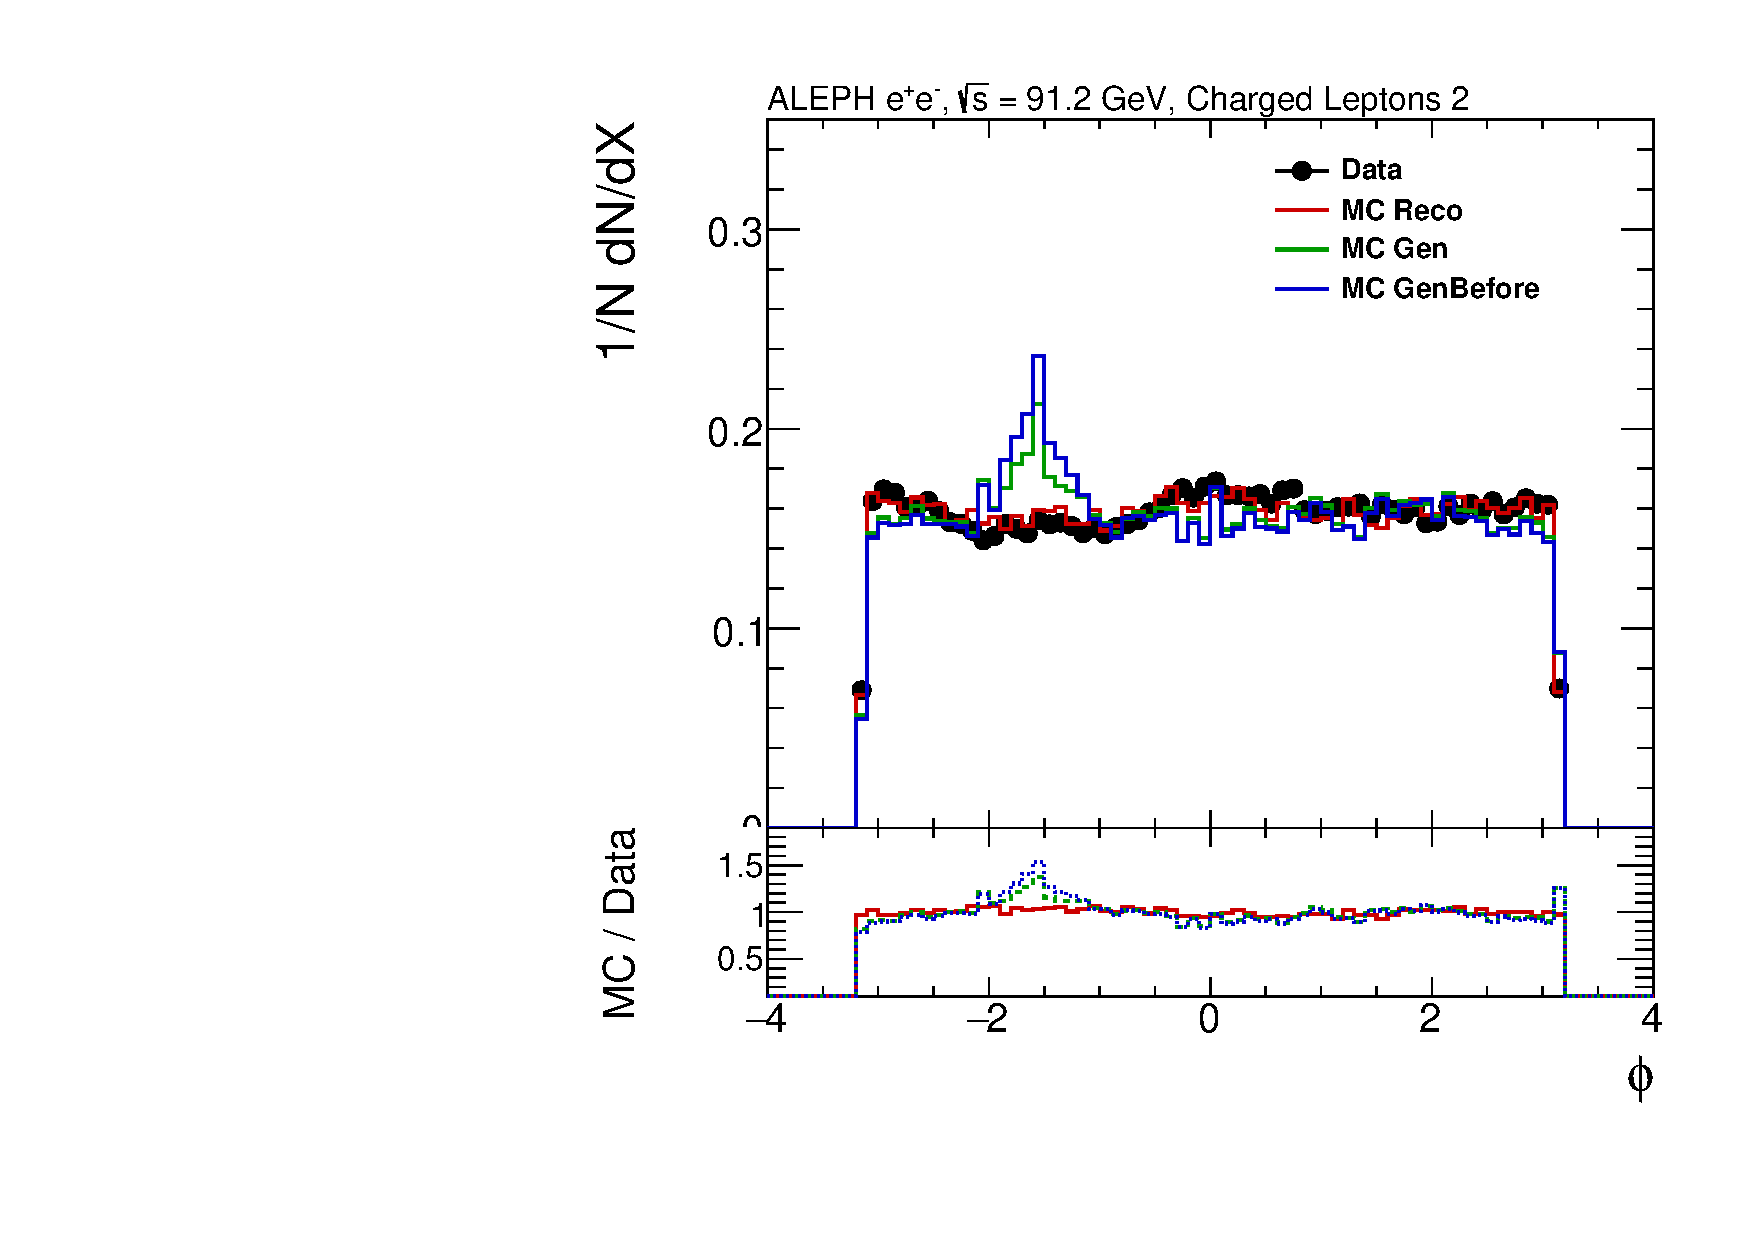
\includegraphics[width=0.325\textwidth]{../Studies/PreliminaryResult/2026-02-17_thrust_iter5/pwflag_kinematics/pwflag2_phi.pdf}
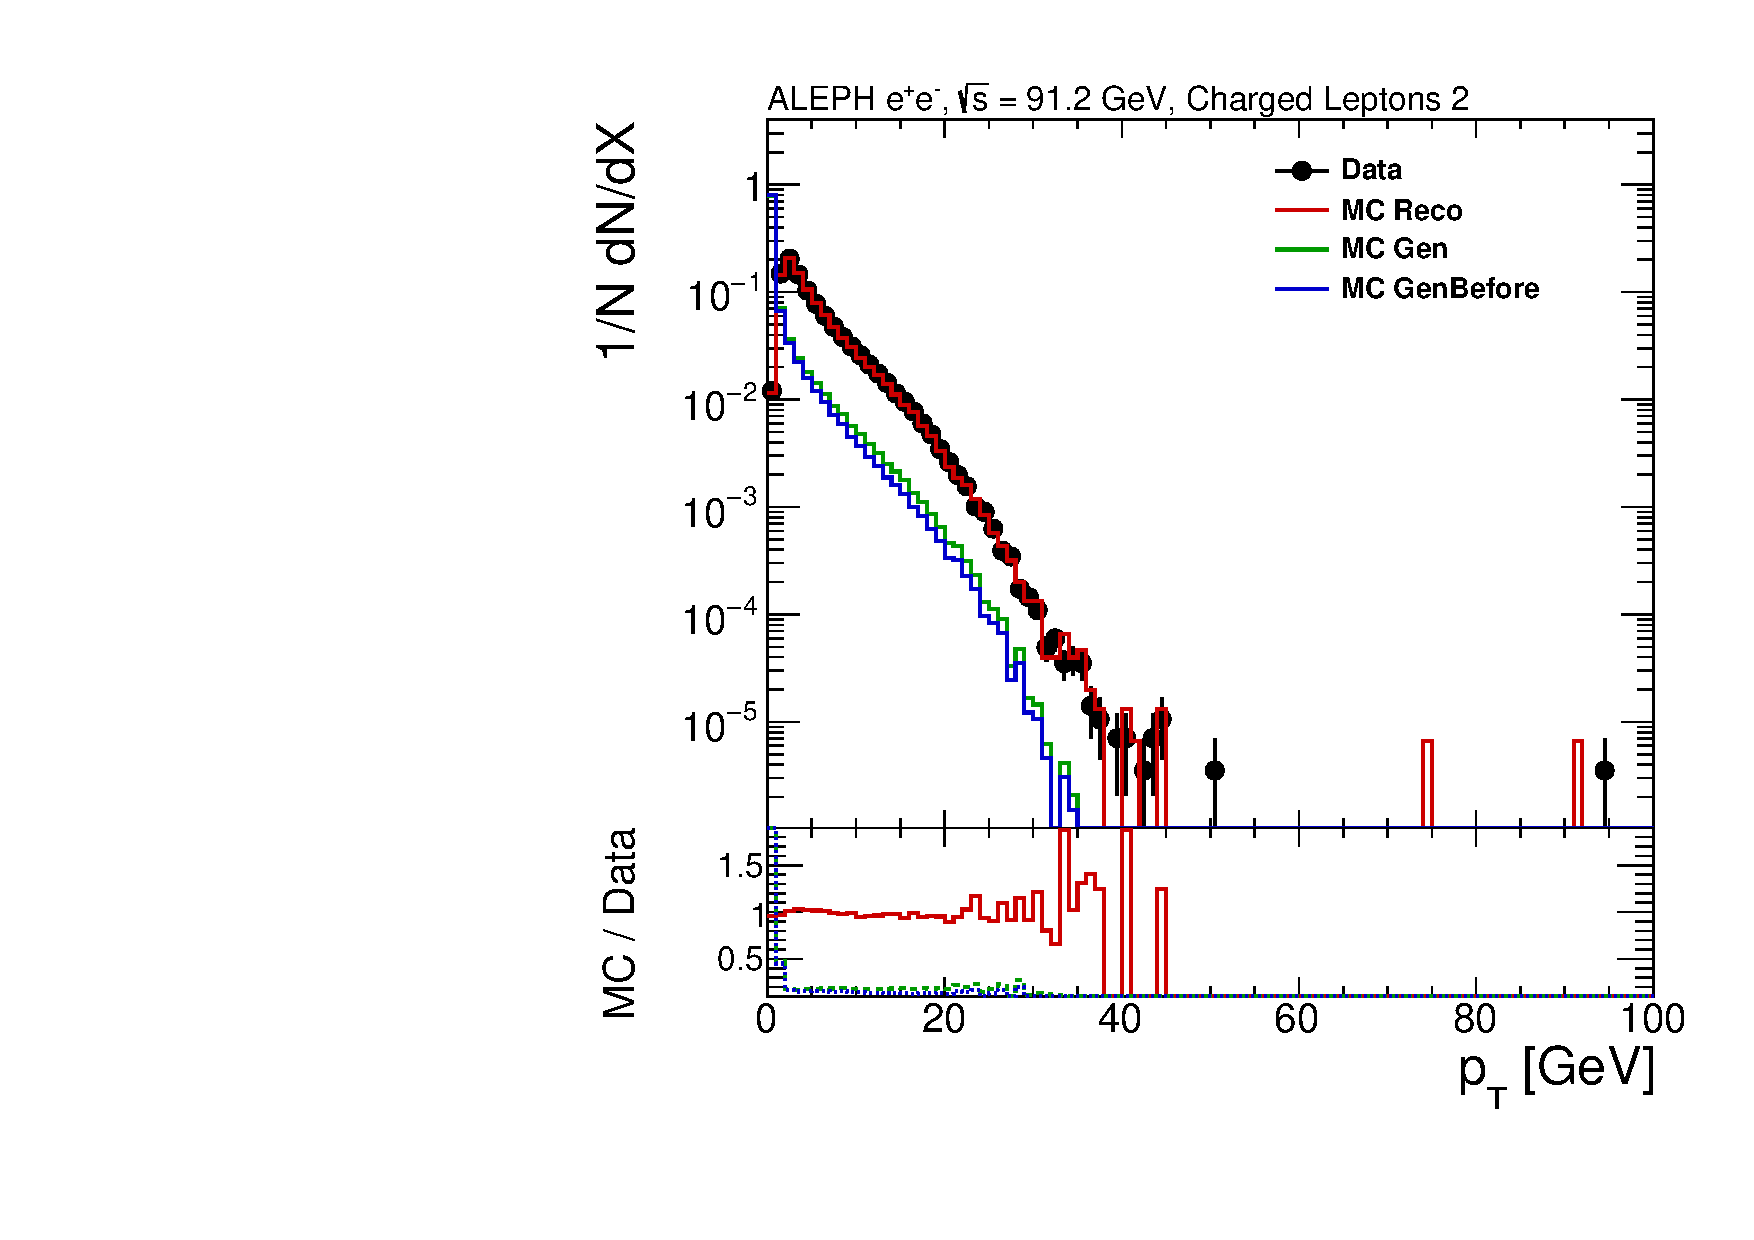
\includegraphics[width=0.325\textwidth]{../Studies/PreliminaryResult/2026-02-17_thrust_iter5/pwflag_kinematics/pwflag2_pt.pdf}
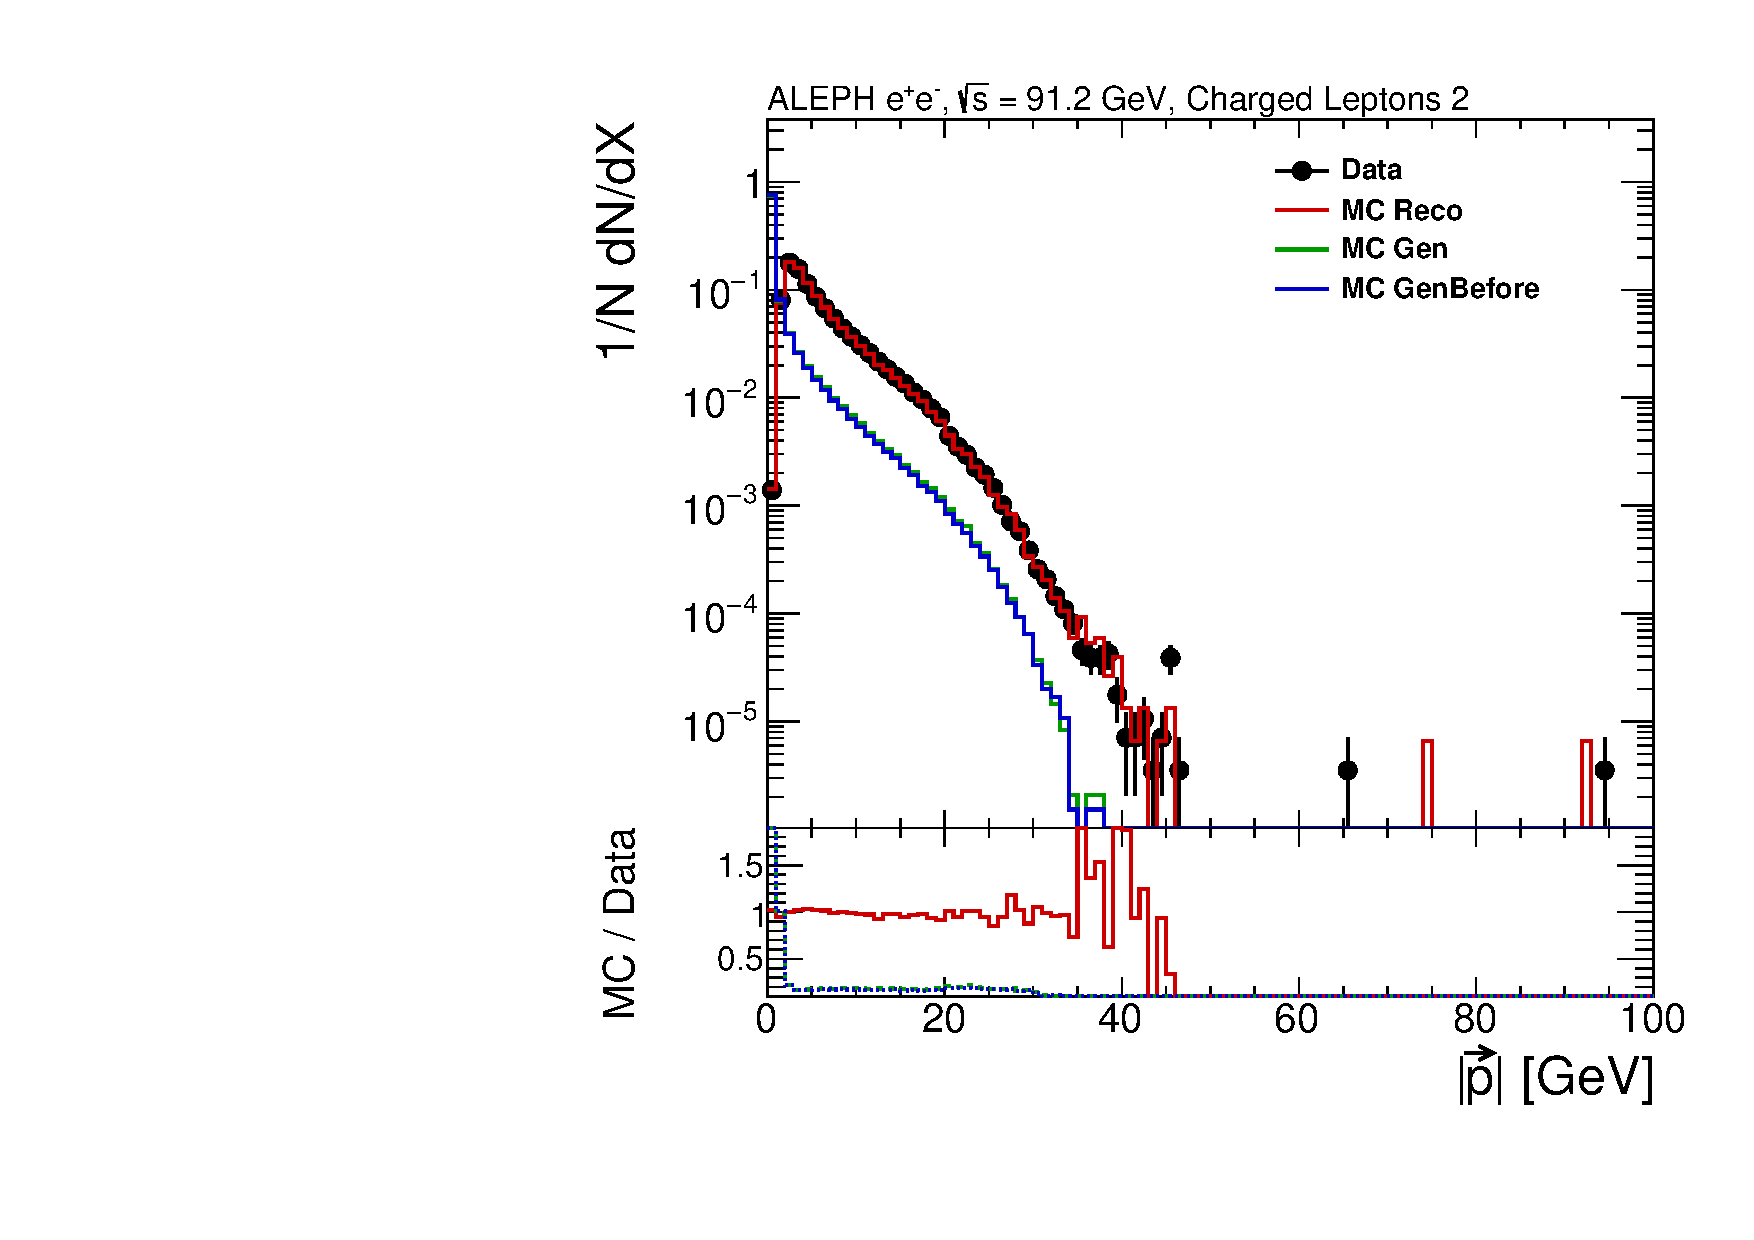
\includegraphics[width=0.325\textwidth]{../Studies/PreliminaryResult/2026-02-17_thrust_iter5/pwflag_kinematics/pwflag2_pmag.pdf}
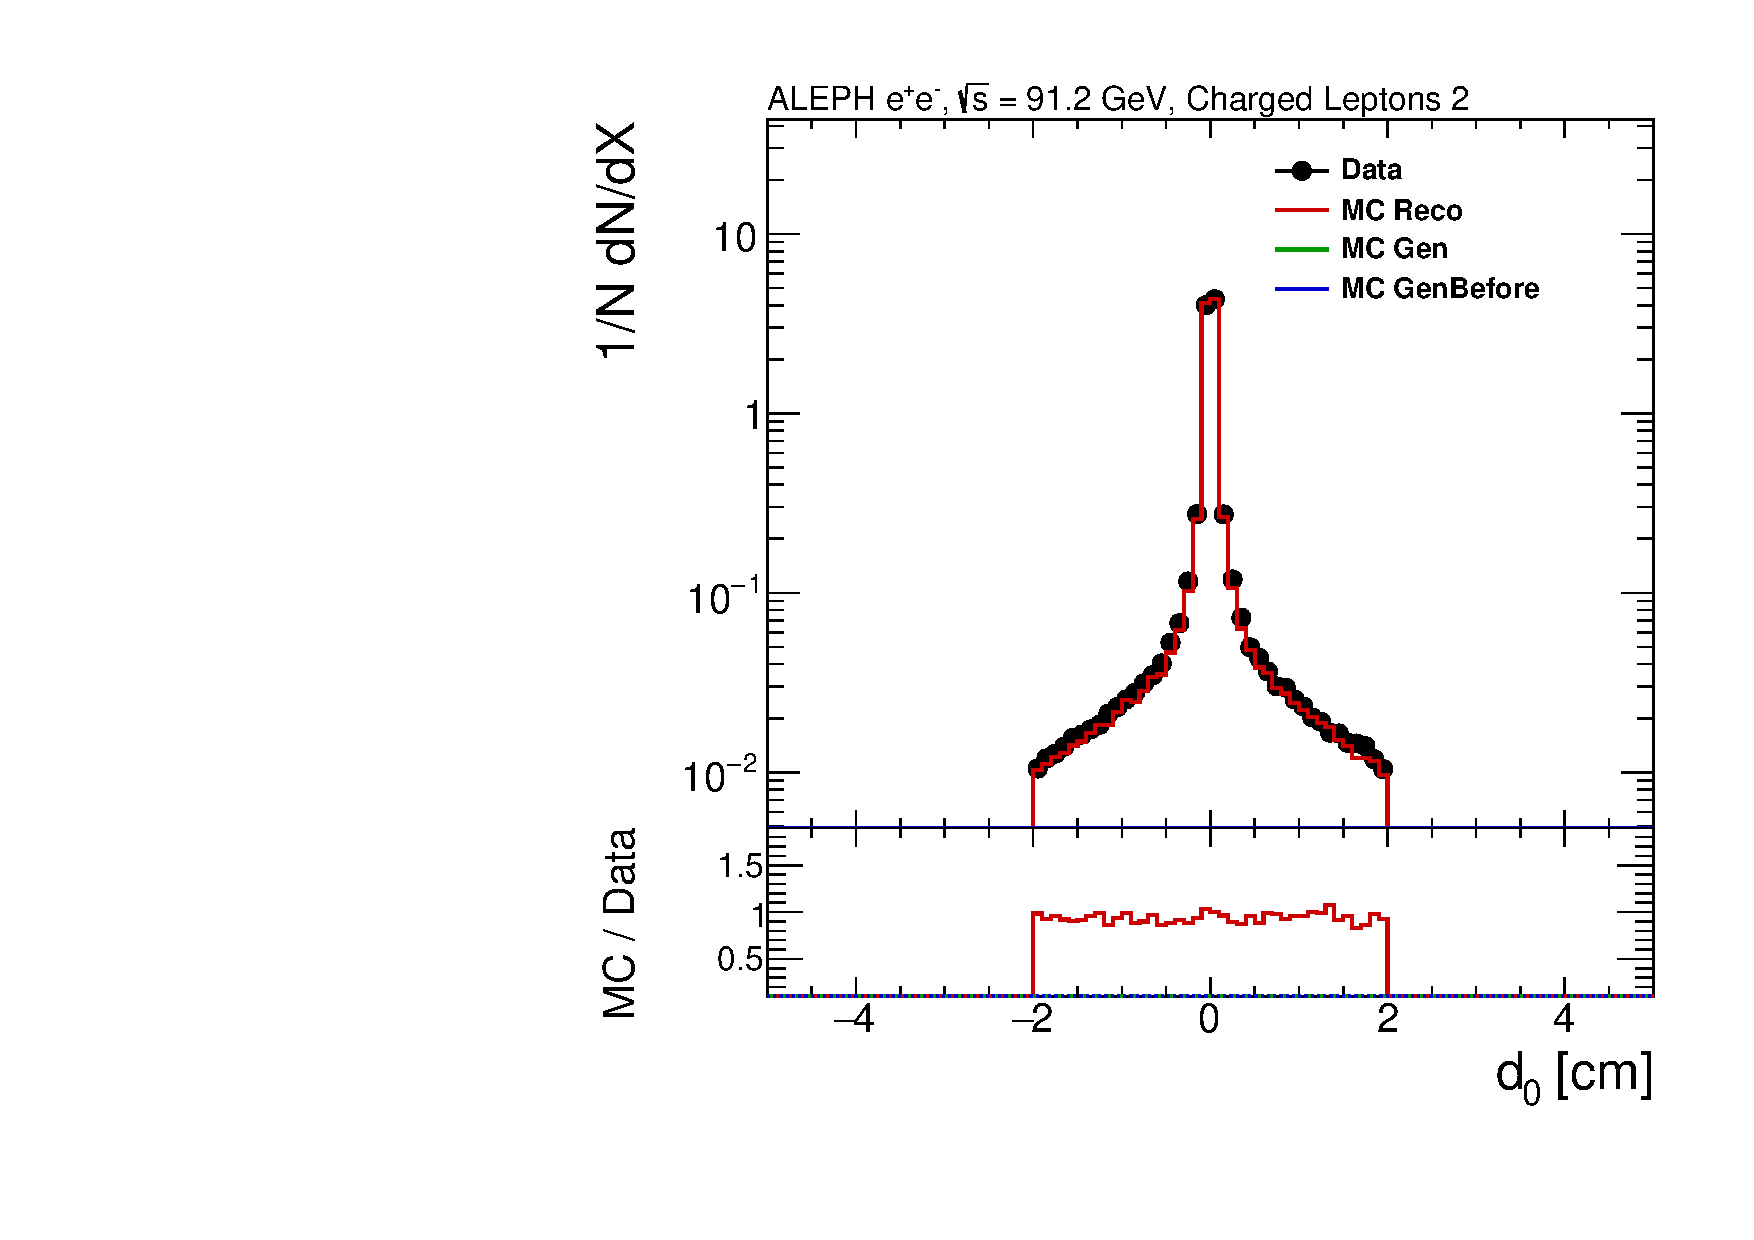
\includegraphics[width=0.325\textwidth]{../Studies/PreliminaryResult/2026-02-17_thrust_iter5/pwflag_kinematics/pwflag2_d0.pdf}
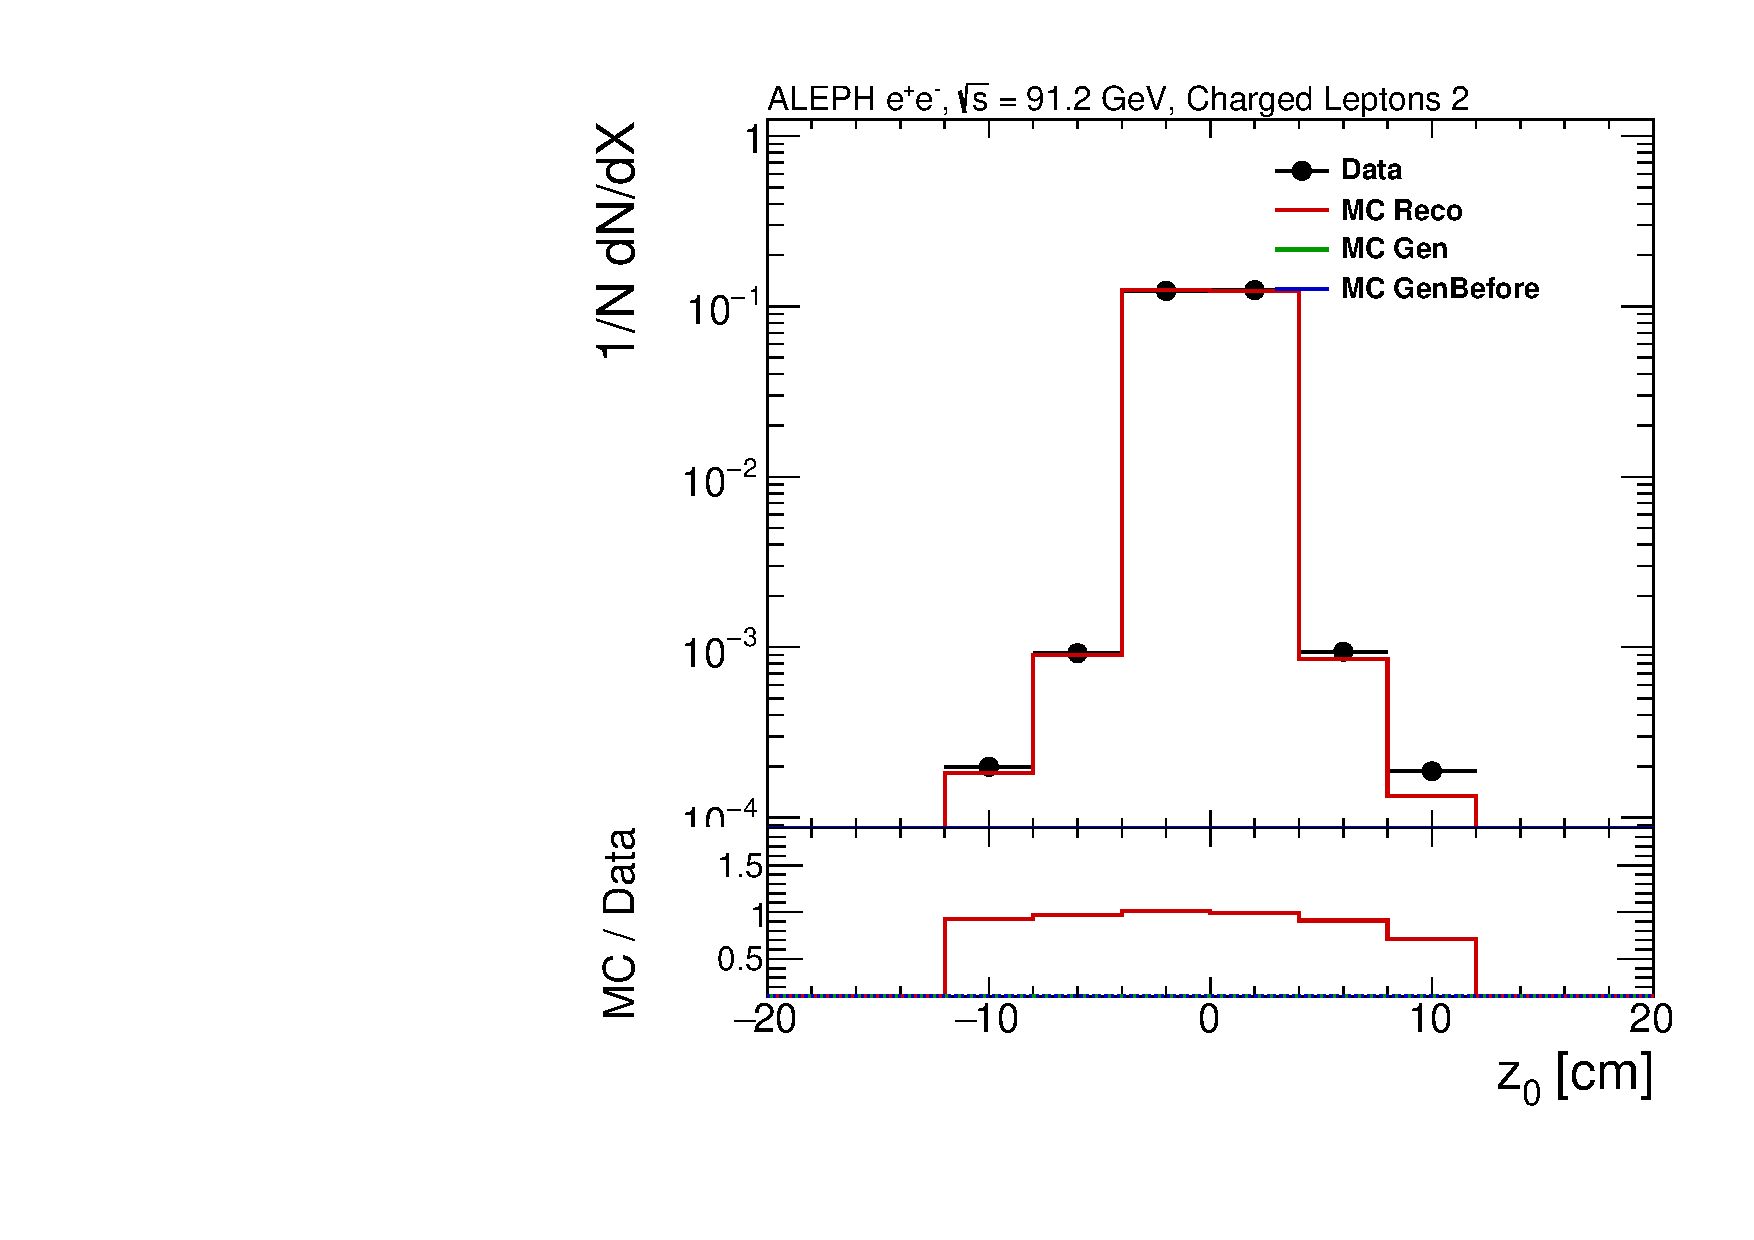
\includegraphics[width=0.325\textwidth]{../Studies/PreliminaryResult/2026-02-17_thrust_iter5/pwflag_kinematics/pwflag2_z0.pdf}
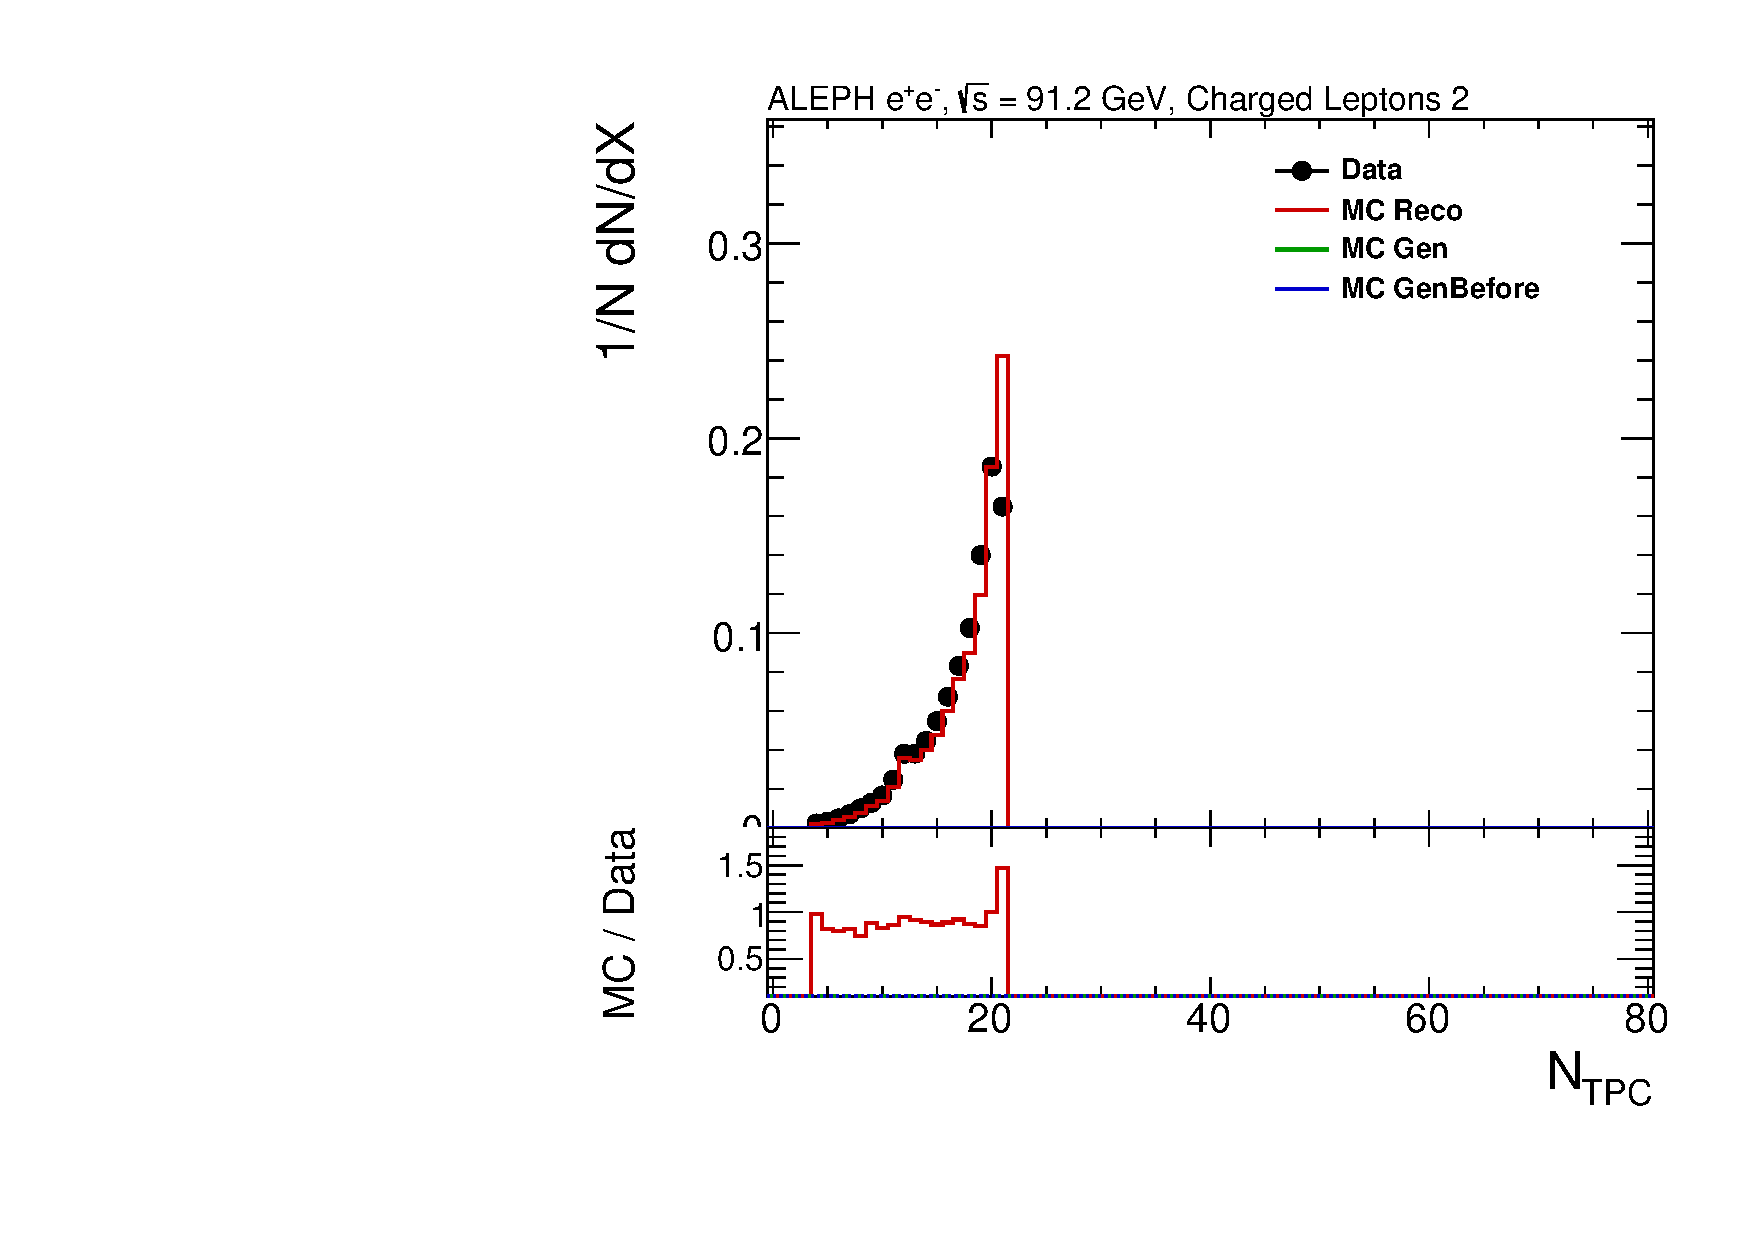
\includegraphics[width=0.325\textwidth]{../Studies/PreliminaryResult/2026-02-17_thrust_iter5/pwflag_kinematics/pwflag2_ntpc.pdf}
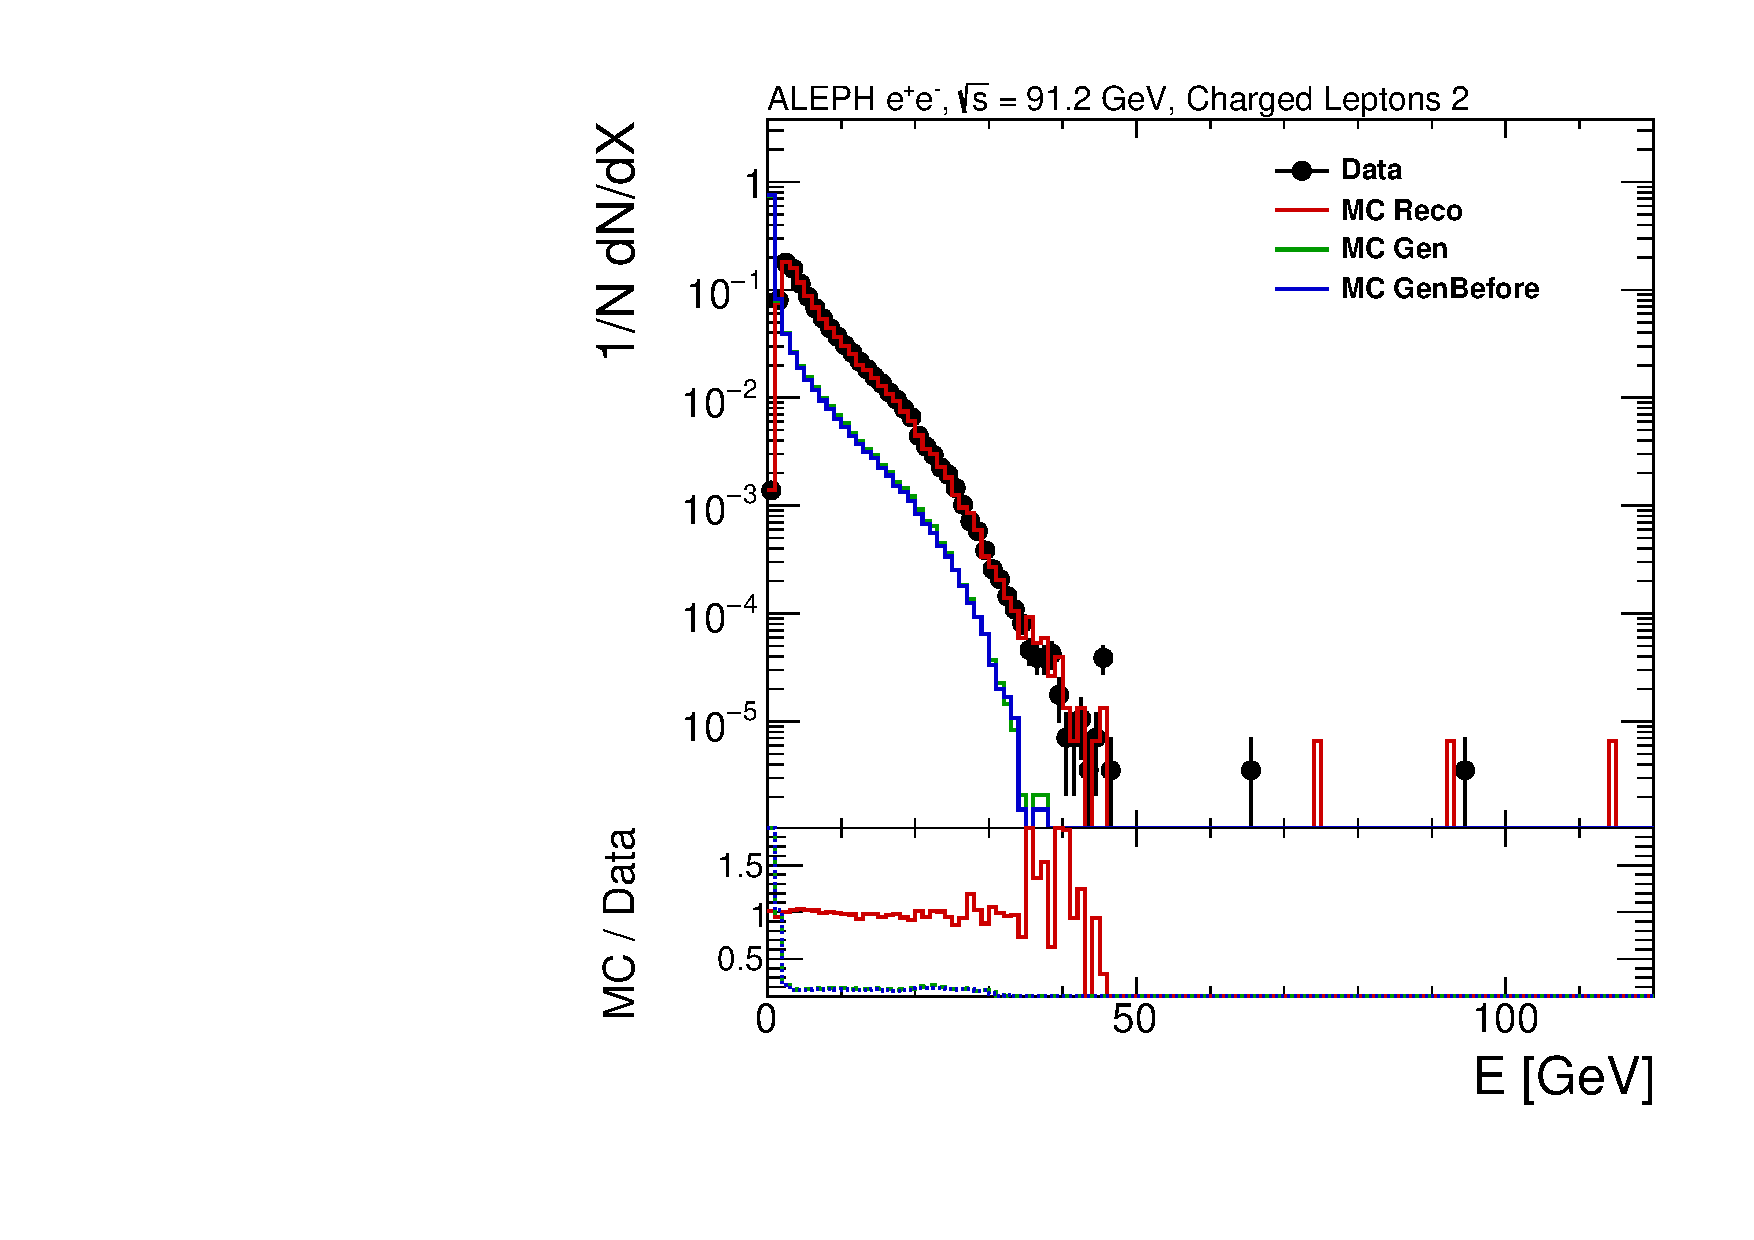
\includegraphics[width=0.325\textwidth]{../Studies/PreliminaryResult/2026-02-17_thrust_iter5/pwflag_kinematics/pwflag2_energy.pdf}
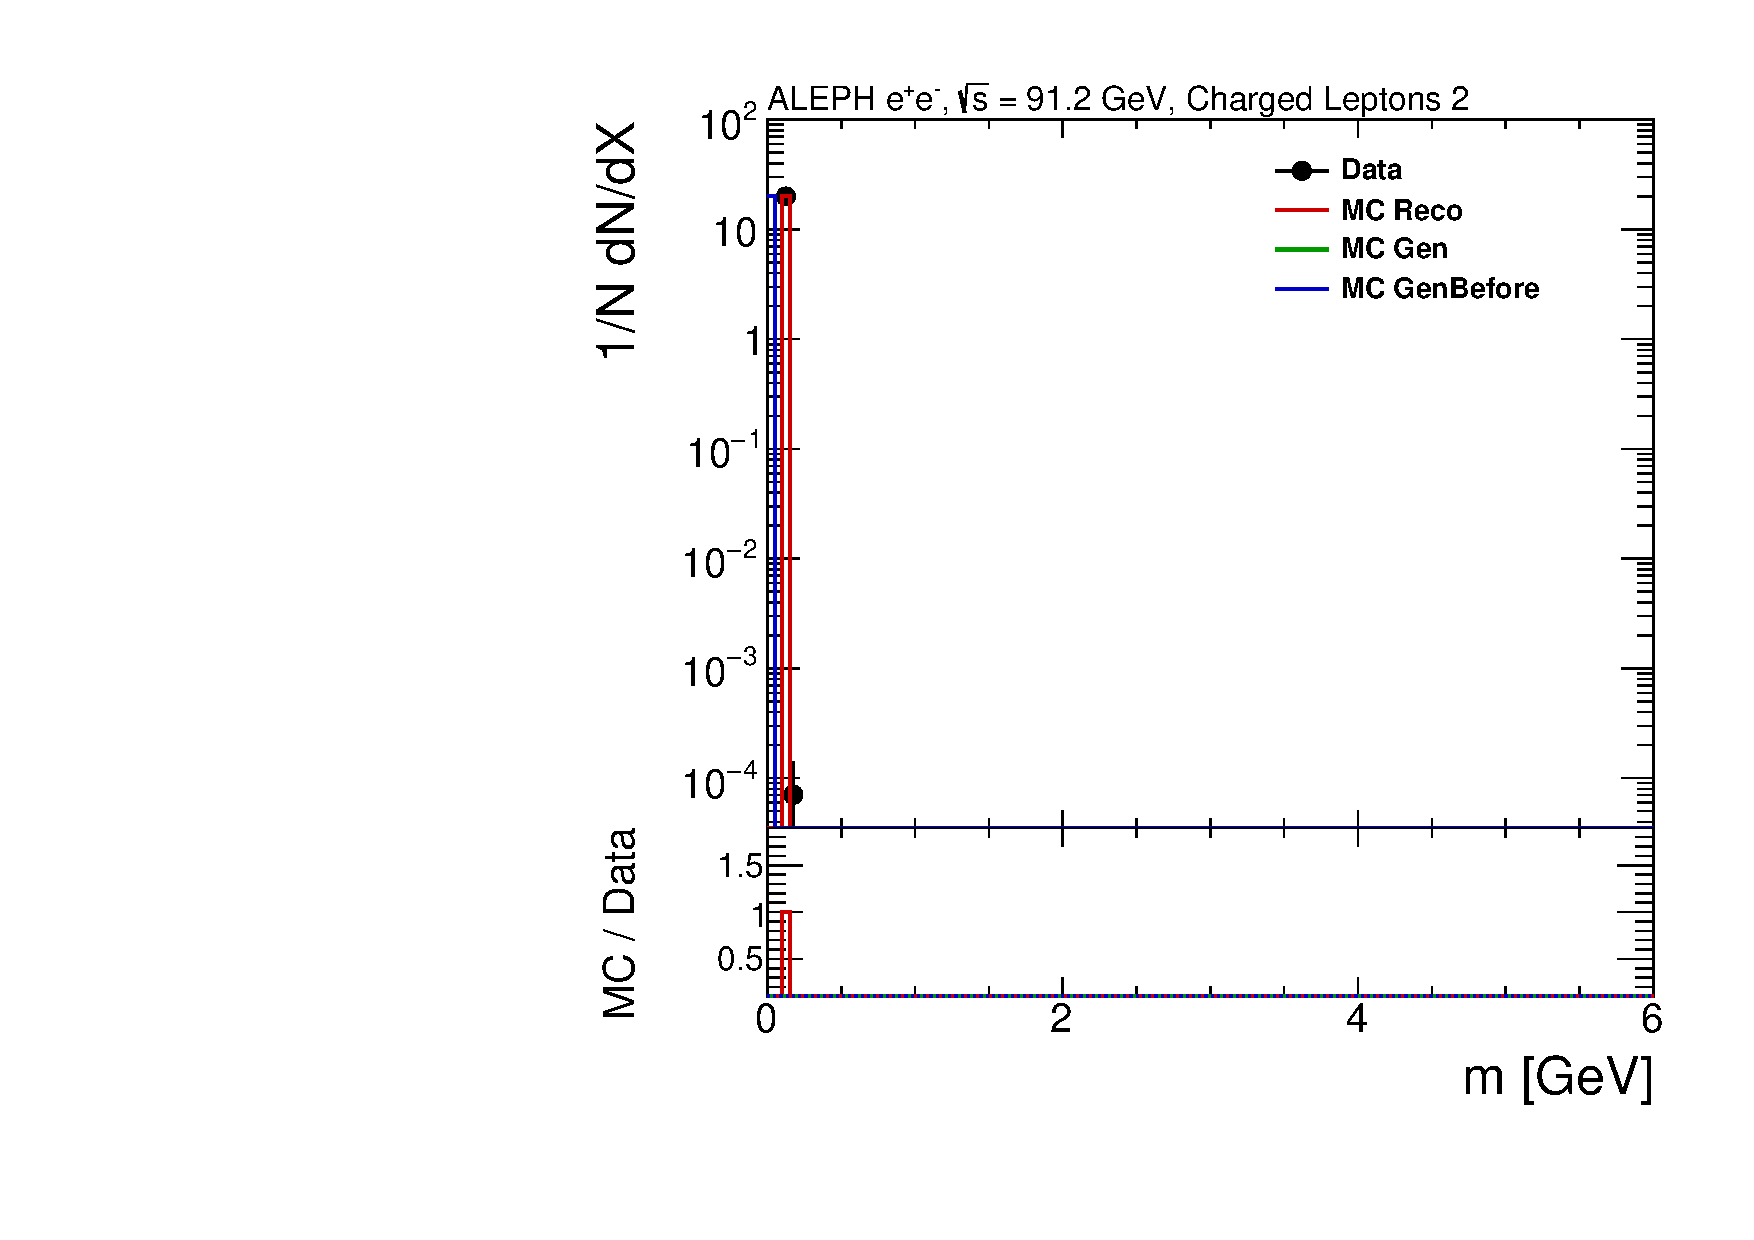
\includegraphics[width=0.325\textwidth]{../Studies/PreliminaryResult/2026-02-17_thrust_iter5/pwflag_kinematics/pwflag2_mass.pdf}
\caption{Complete \texttt{pwflag}=2 kinematic set.}
\label{fig:pwflag2_full}
\end{figure}

\noindent
Figure~\ref{fig:pwflag2_full} presents the second charged-lepton category, providing a direct
cross-check of category-dependent acceptance and momentum-shape modeling. This category probes
objects with different subdetector signatures than Fig.~\ref{fig:pwflag1_full}, so agreement
here confirms that lepton-category partitioning does not induce a hidden detector asymmetry in
the thrust inputs. The high-$p_T$ and high-energy tails are monitored explicitly because even a
small mismodeling there can project onto endpoint thrust bins.

\begin{figure}[t!]
\centering
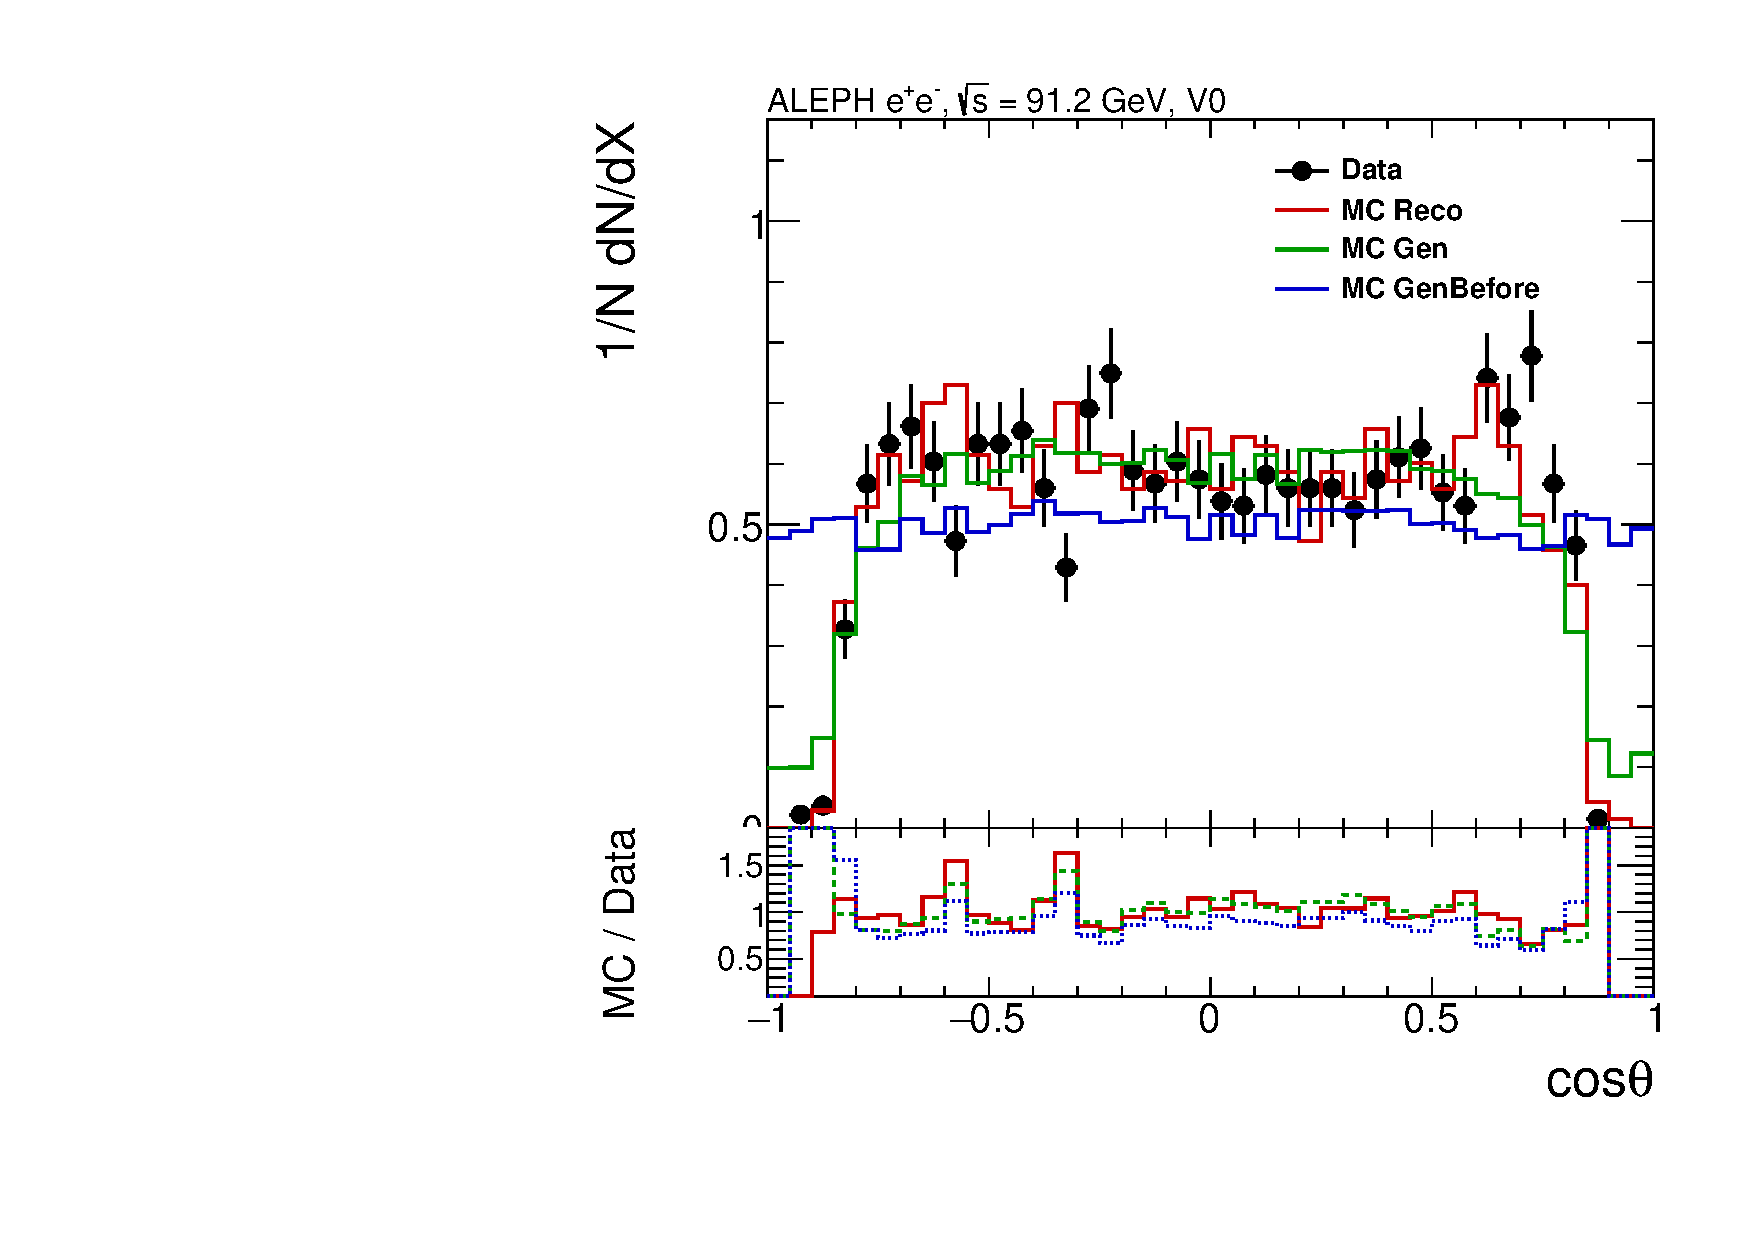
\includegraphics[width=0.325\textwidth]{../Studies/PreliminaryResult/2026-02-17_thrust_iter5/pwflag_kinematics/pwflag3_cosTheta.pdf}
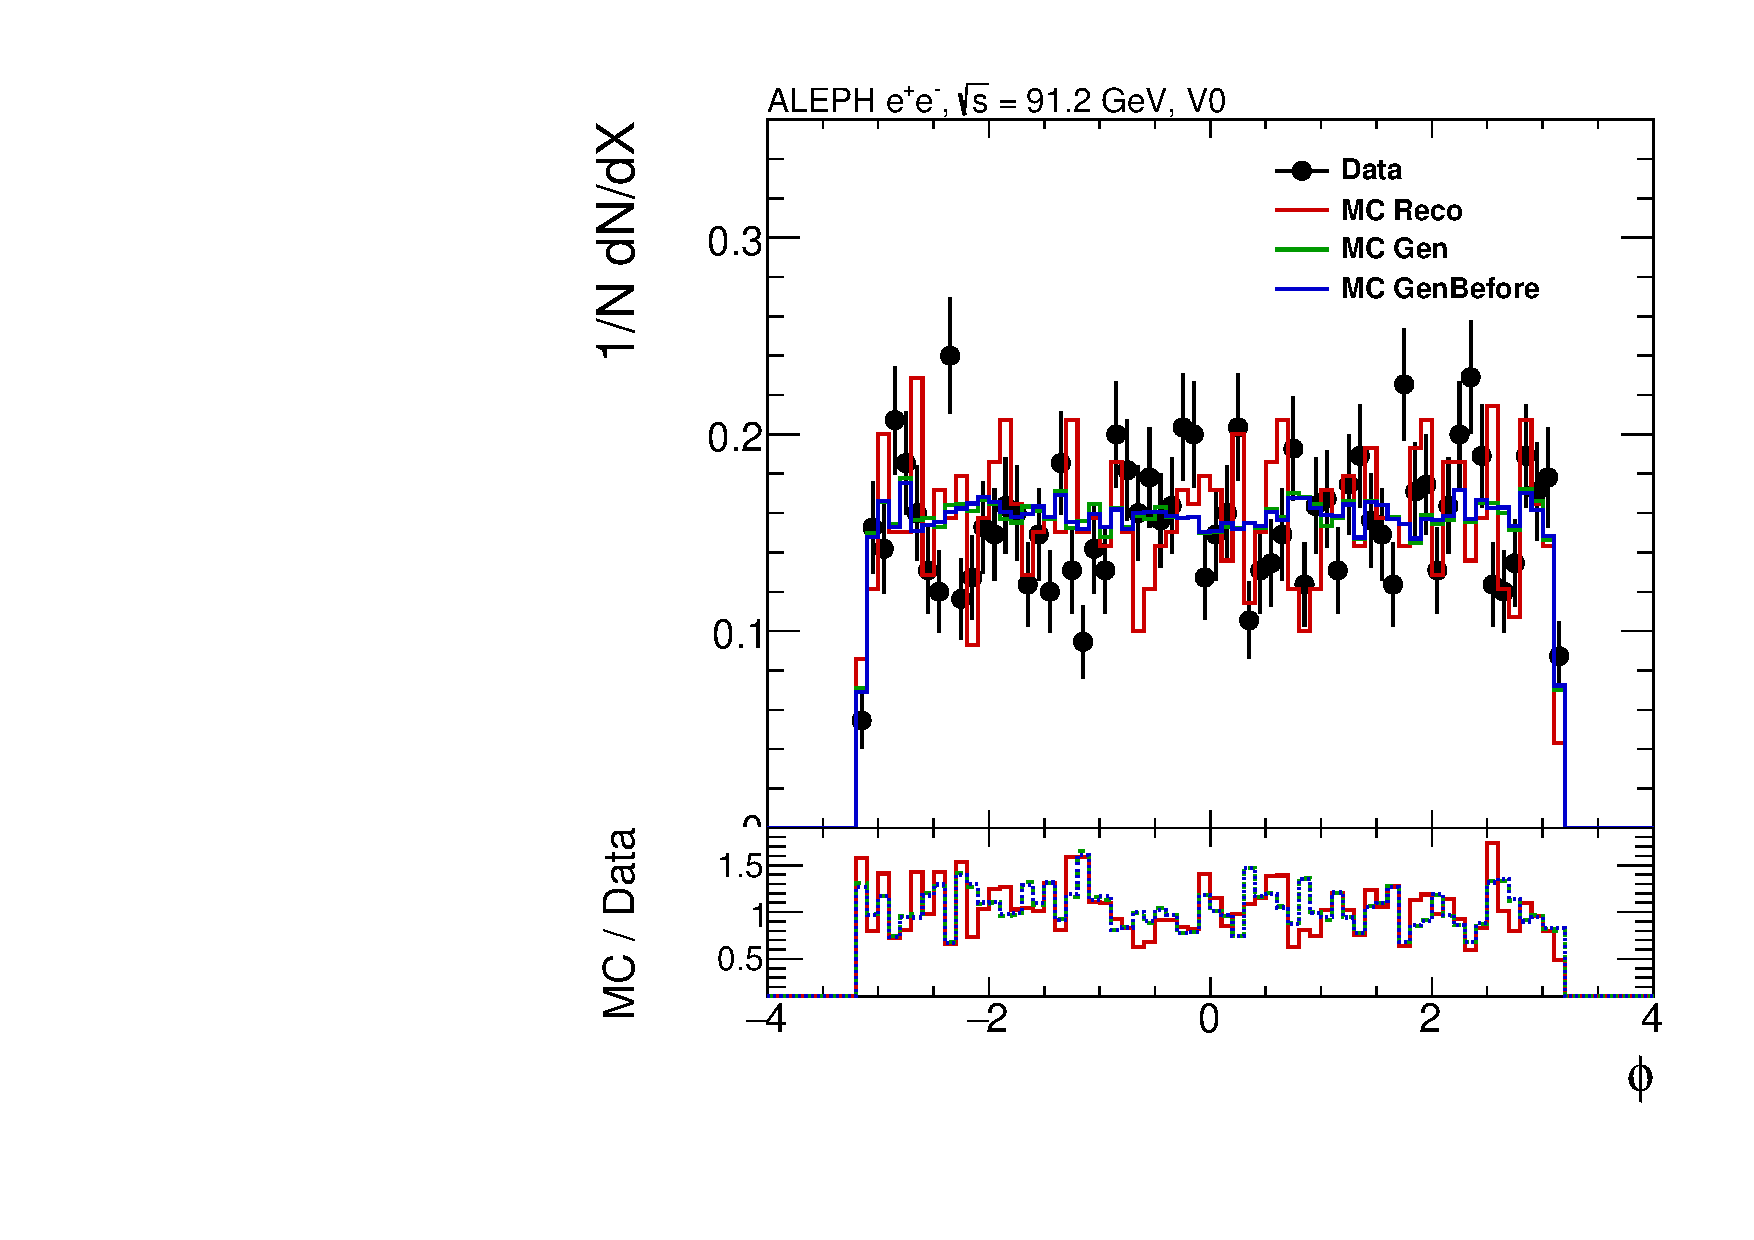
\includegraphics[width=0.325\textwidth]{../Studies/PreliminaryResult/2026-02-17_thrust_iter5/pwflag_kinematics/pwflag3_phi.pdf}
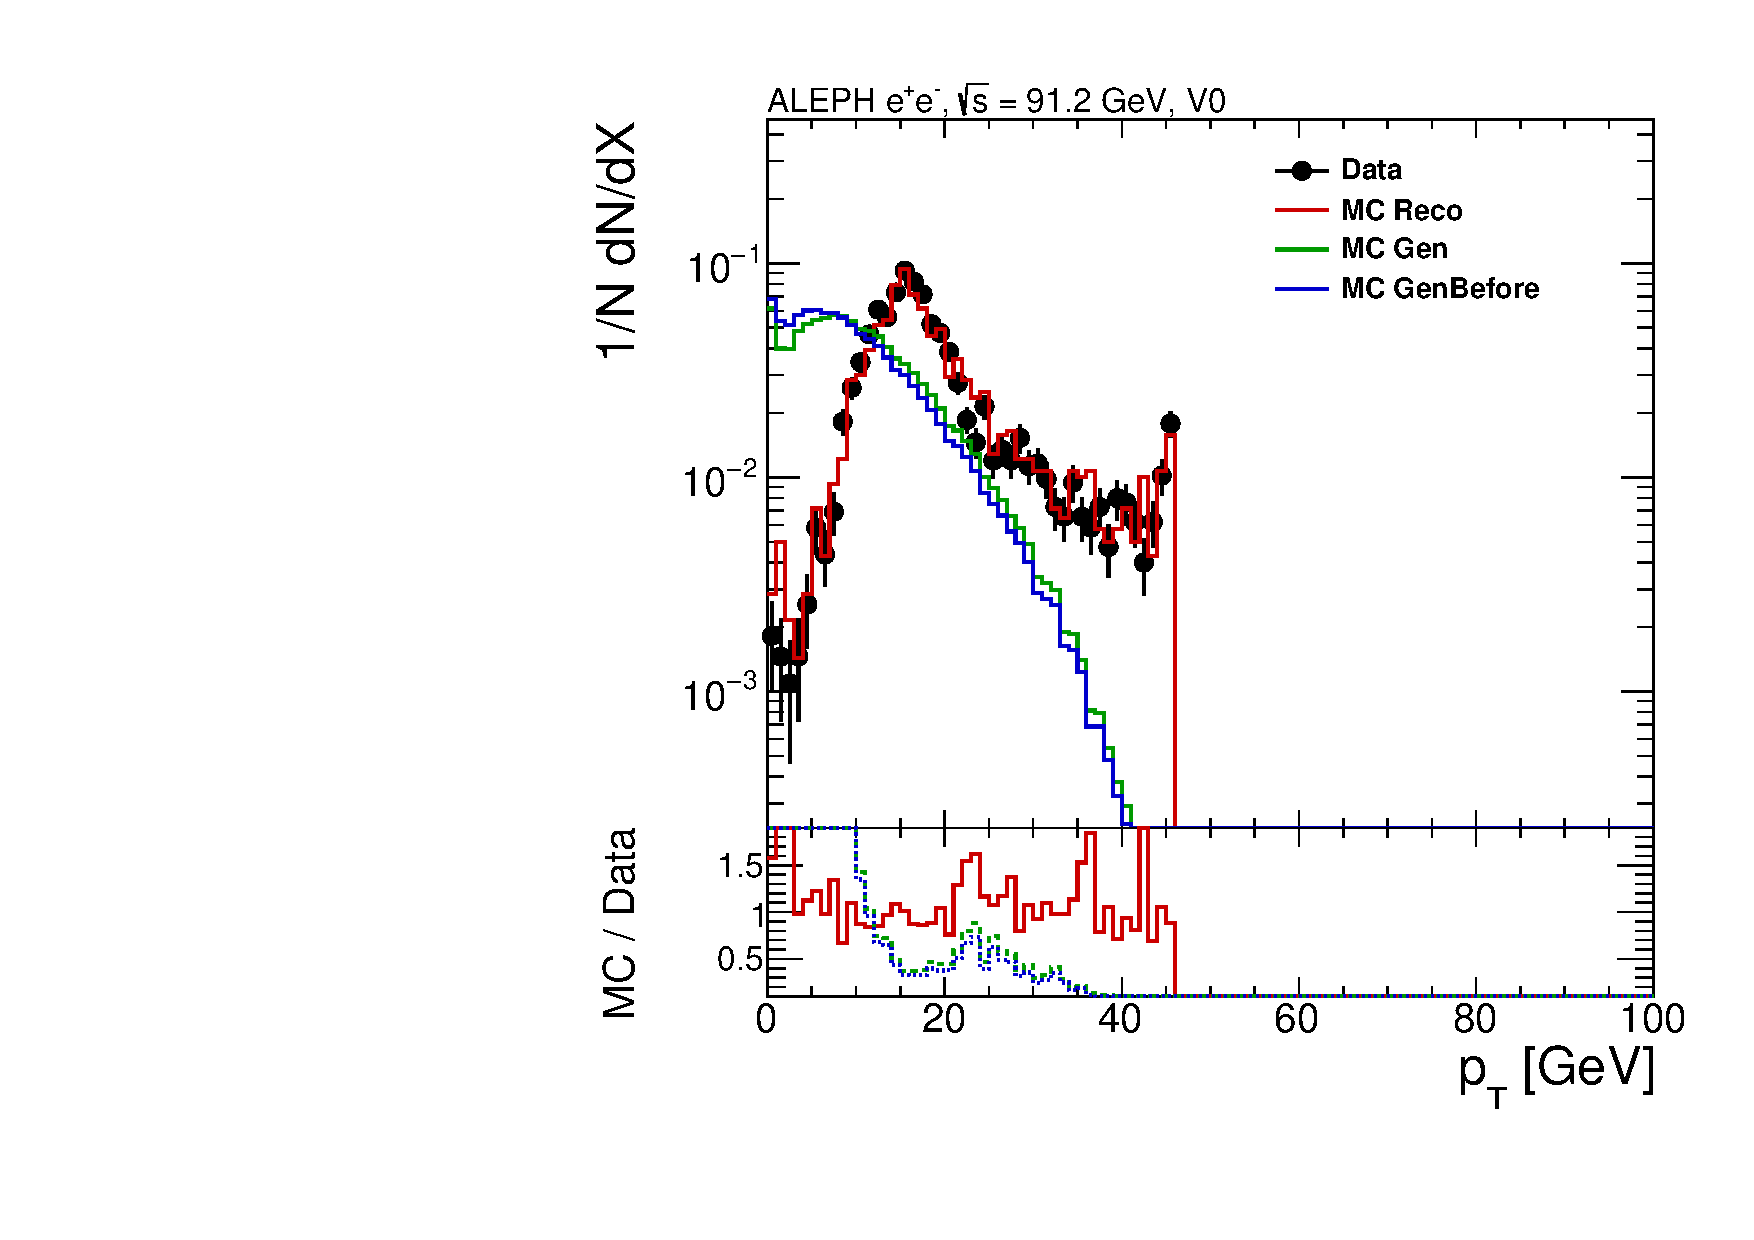
\includegraphics[width=0.325\textwidth]{../Studies/PreliminaryResult/2026-02-17_thrust_iter5/pwflag_kinematics/pwflag3_pt.pdf}
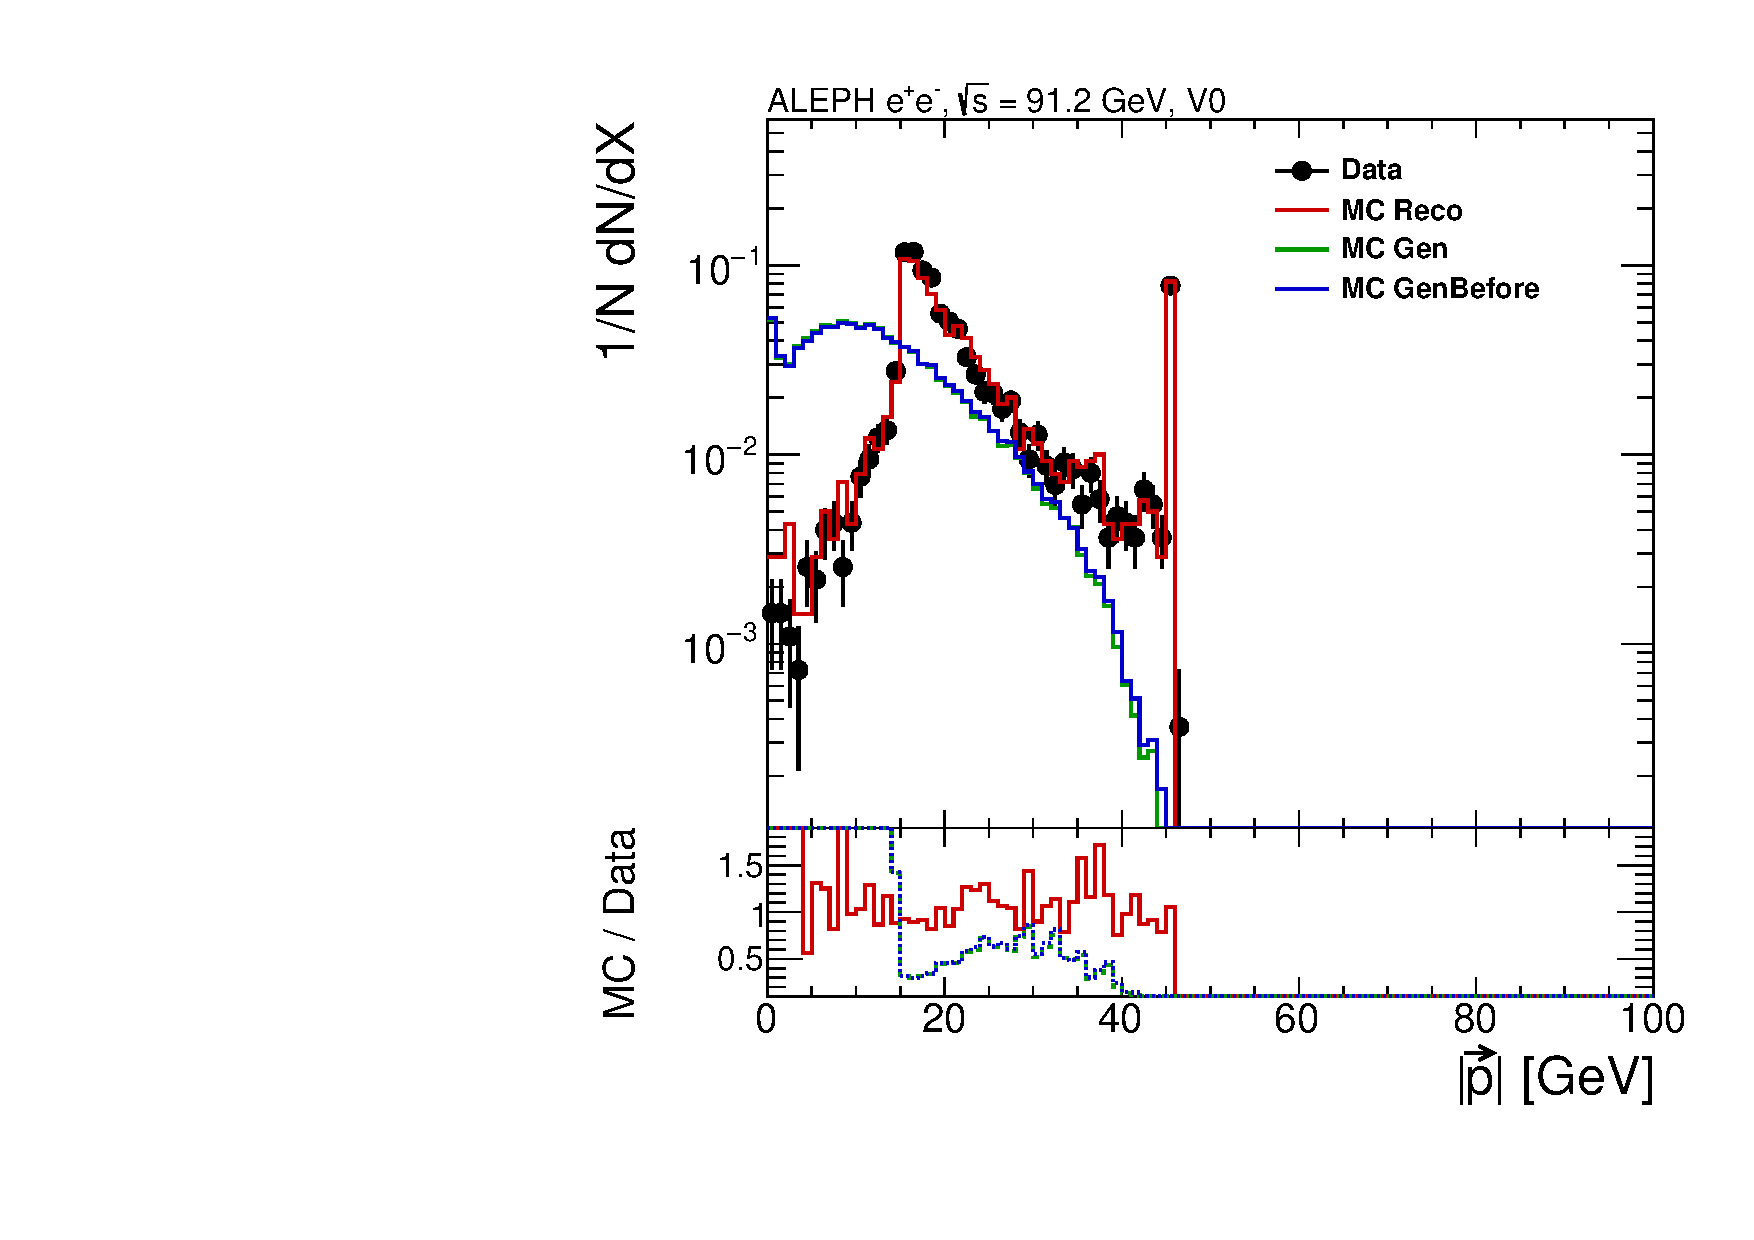
\includegraphics[width=0.325\textwidth]{../Studies/PreliminaryResult/2026-02-17_thrust_iter5/pwflag_kinematics/pwflag3_pmag.pdf}
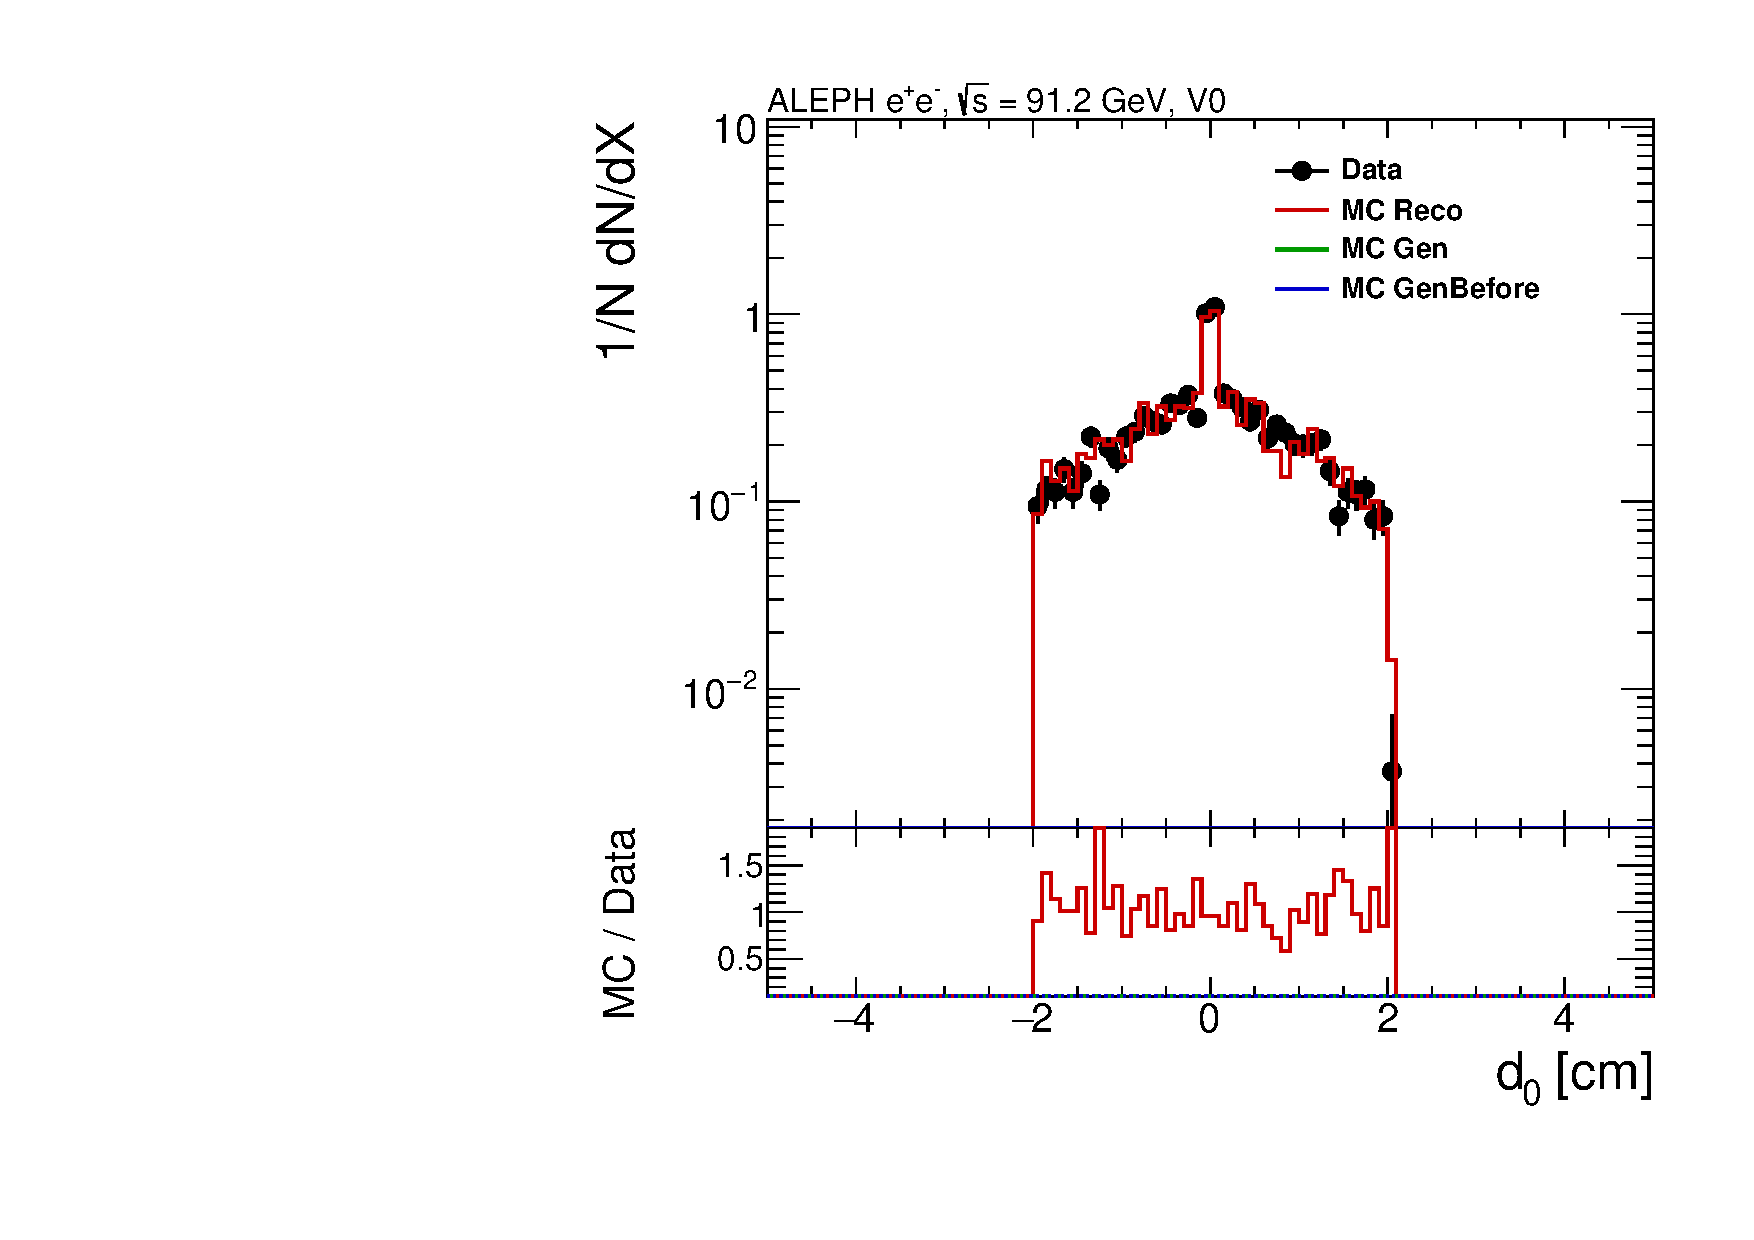
\includegraphics[width=0.325\textwidth]{../Studies/PreliminaryResult/2026-02-17_thrust_iter5/pwflag_kinematics/pwflag3_d0.pdf}
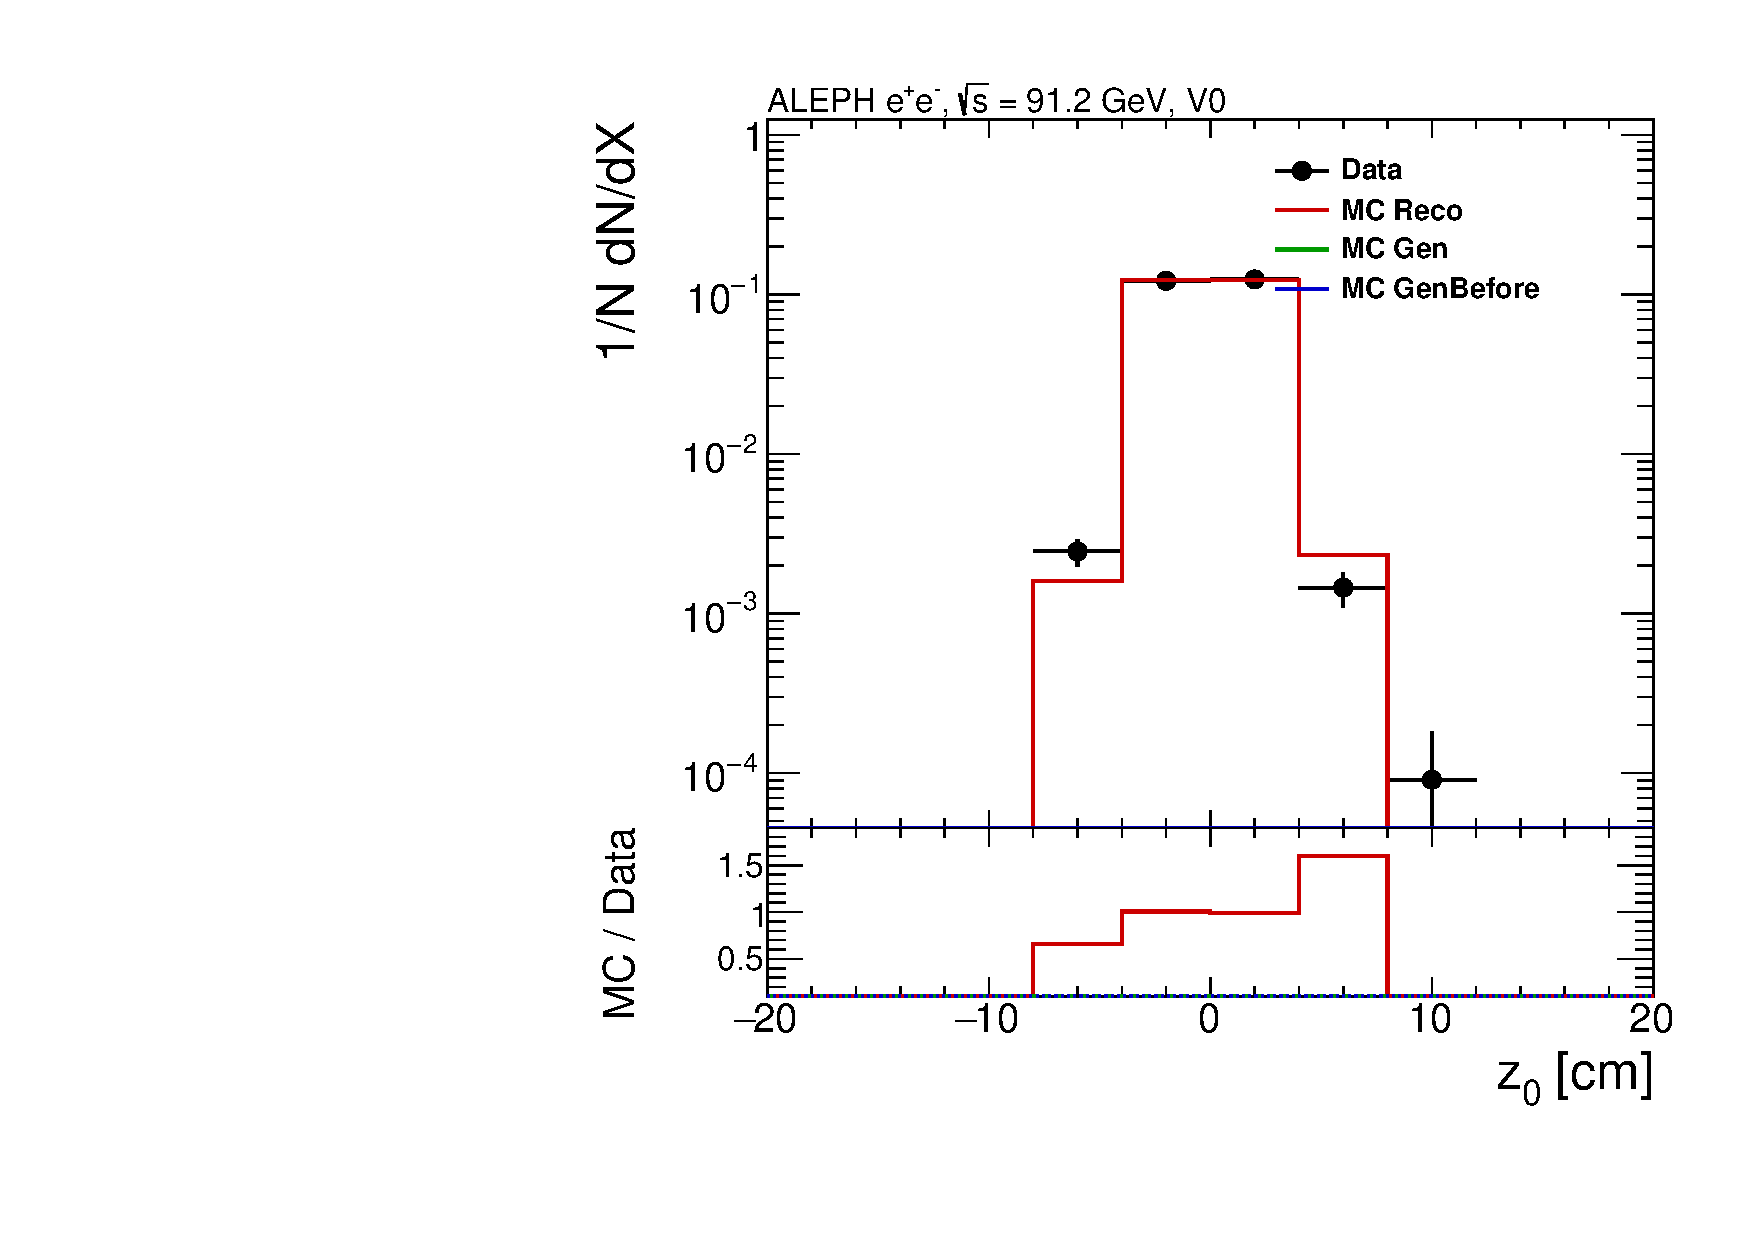
\includegraphics[width=0.325\textwidth]{../Studies/PreliminaryResult/2026-02-17_thrust_iter5/pwflag_kinematics/pwflag3_z0.pdf}
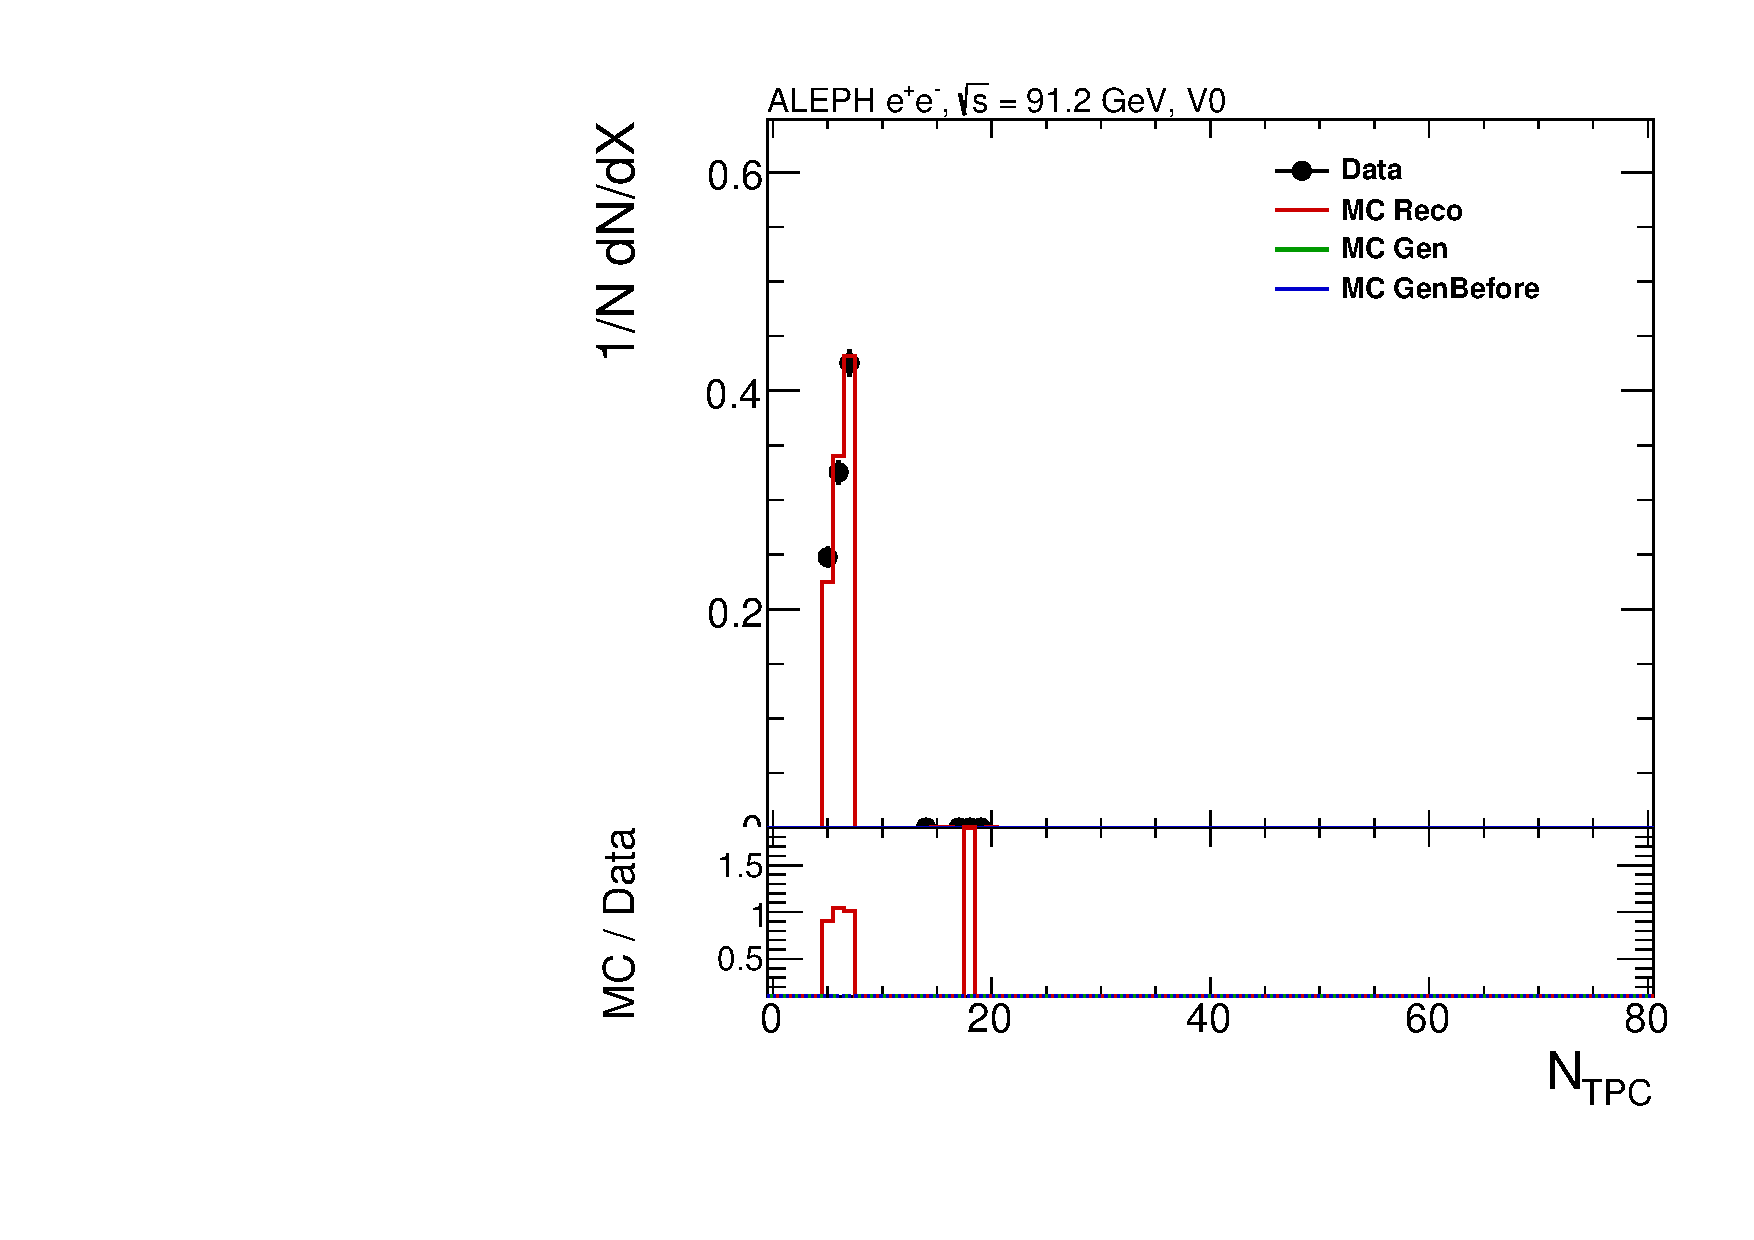
\includegraphics[width=0.325\textwidth]{../Studies/PreliminaryResult/2026-02-17_thrust_iter5/pwflag_kinematics/pwflag3_ntpc.pdf}
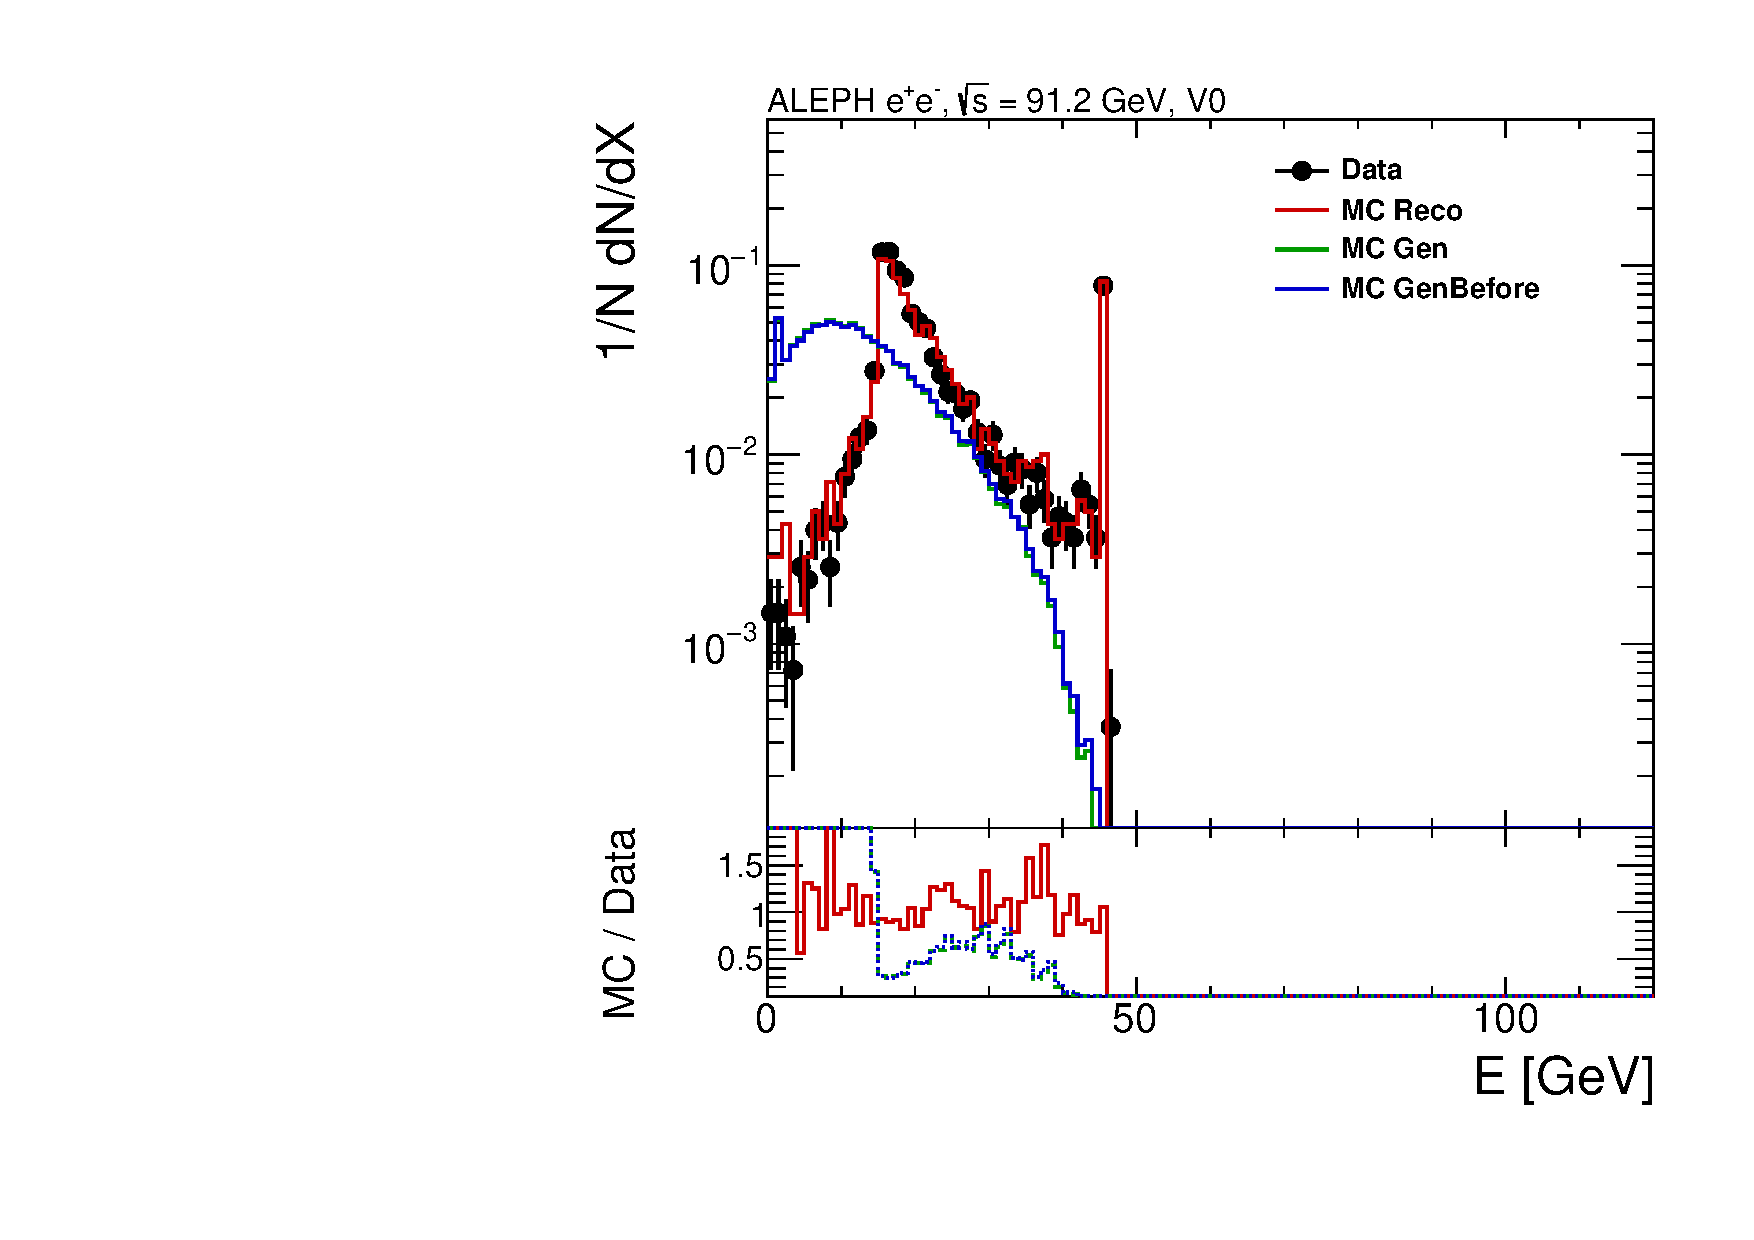
\includegraphics[width=0.325\textwidth]{../Studies/PreliminaryResult/2026-02-17_thrust_iter5/pwflag_kinematics/pwflag3_energy.pdf}
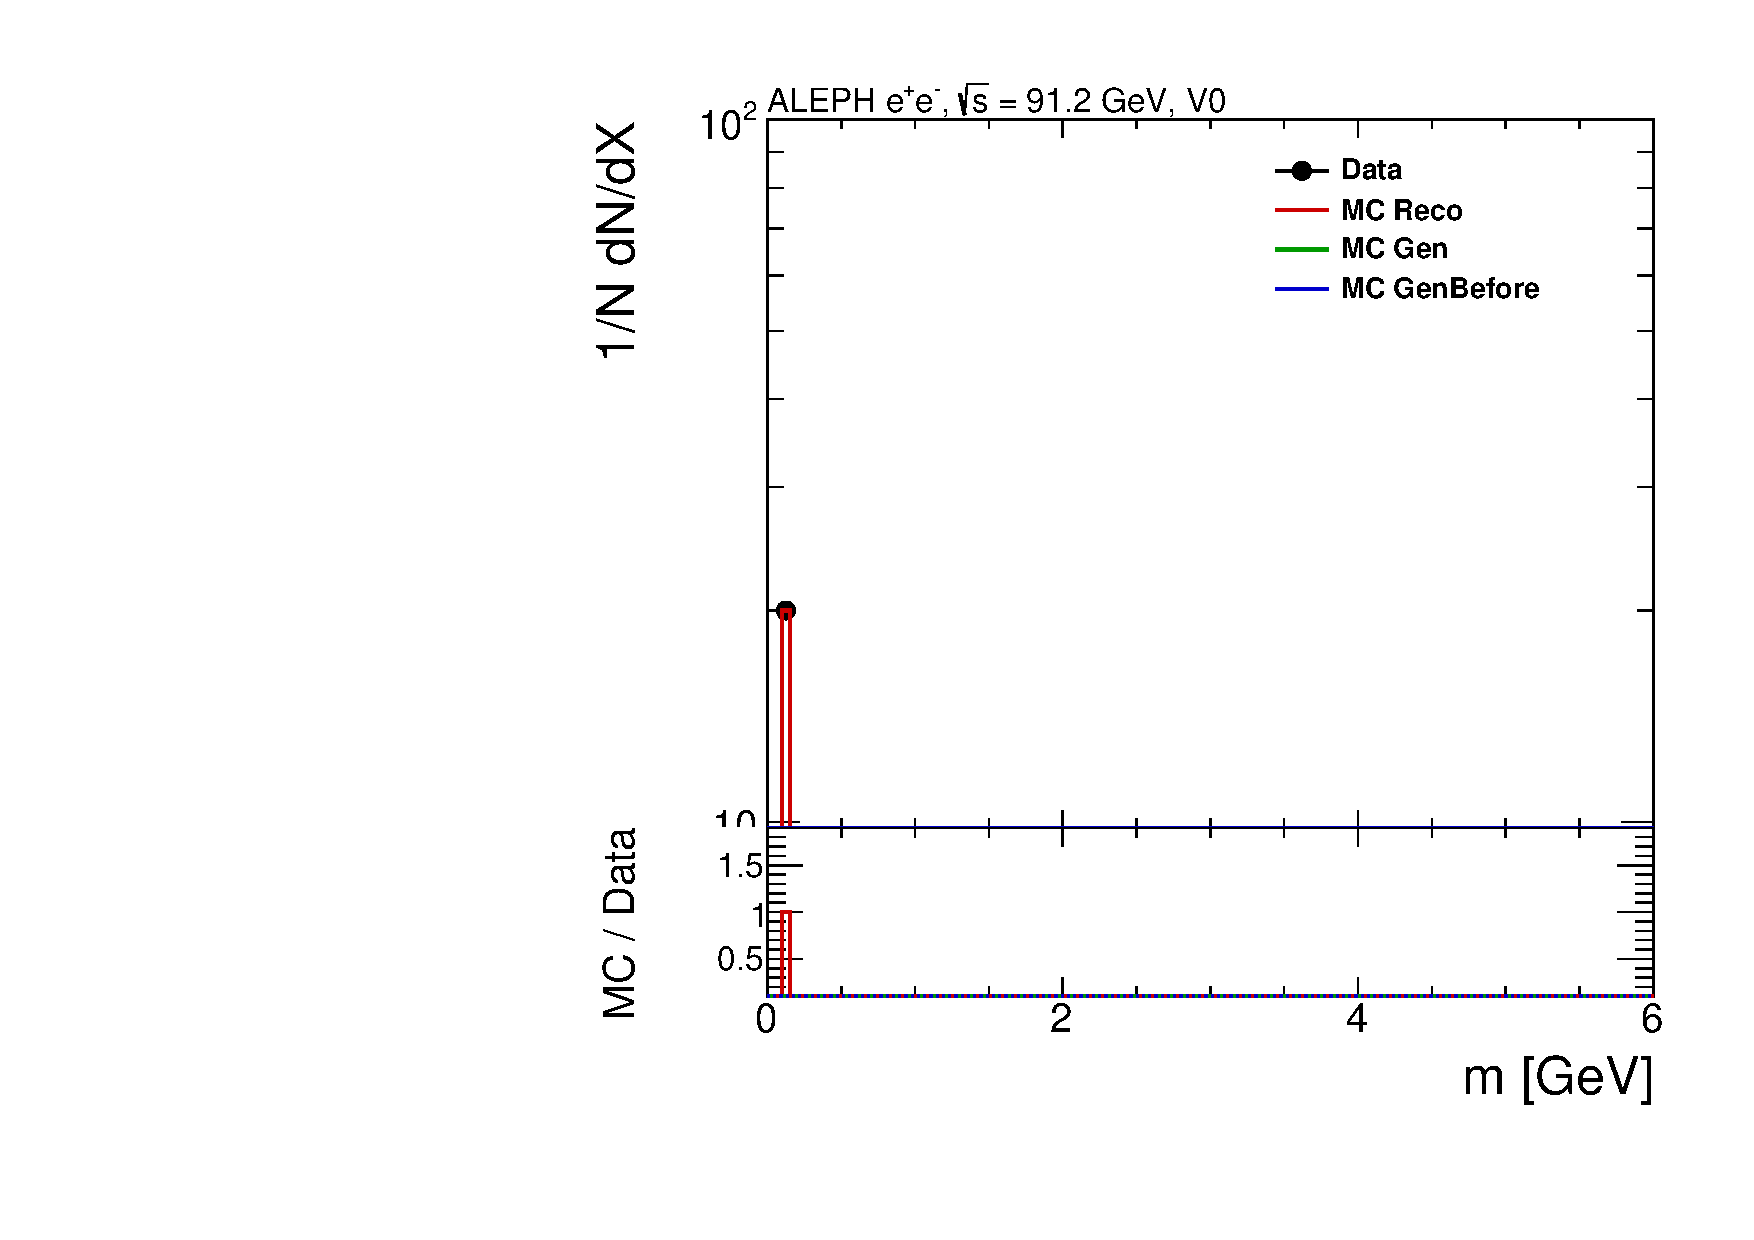
\includegraphics[width=0.325\textwidth]{../Studies/PreliminaryResult/2026-02-17_thrust_iter5/pwflag_kinematics/pwflag3_mass.pdf}
\caption{Complete \texttt{pwflag}=3 kinematic set.}
\label{fig:pwflag3_full}
\end{figure}

\noindent
Figure~\ref{fig:pwflag3_full} begins the neutral-object categories, where angular and energy
modeling are especially relevant for visible-energy flow in thrust reconstruction. For this
category, the energy spectrum and angular acceptance are the primary physics handles for event
shape modeling, while the track-like quantities provide consistency checks of the archived object
classification. Agreement in this panel supports a controlled transfer of neutral energy flow into
the unfolded thrust response.

\begin{figure}[t!]
\centering
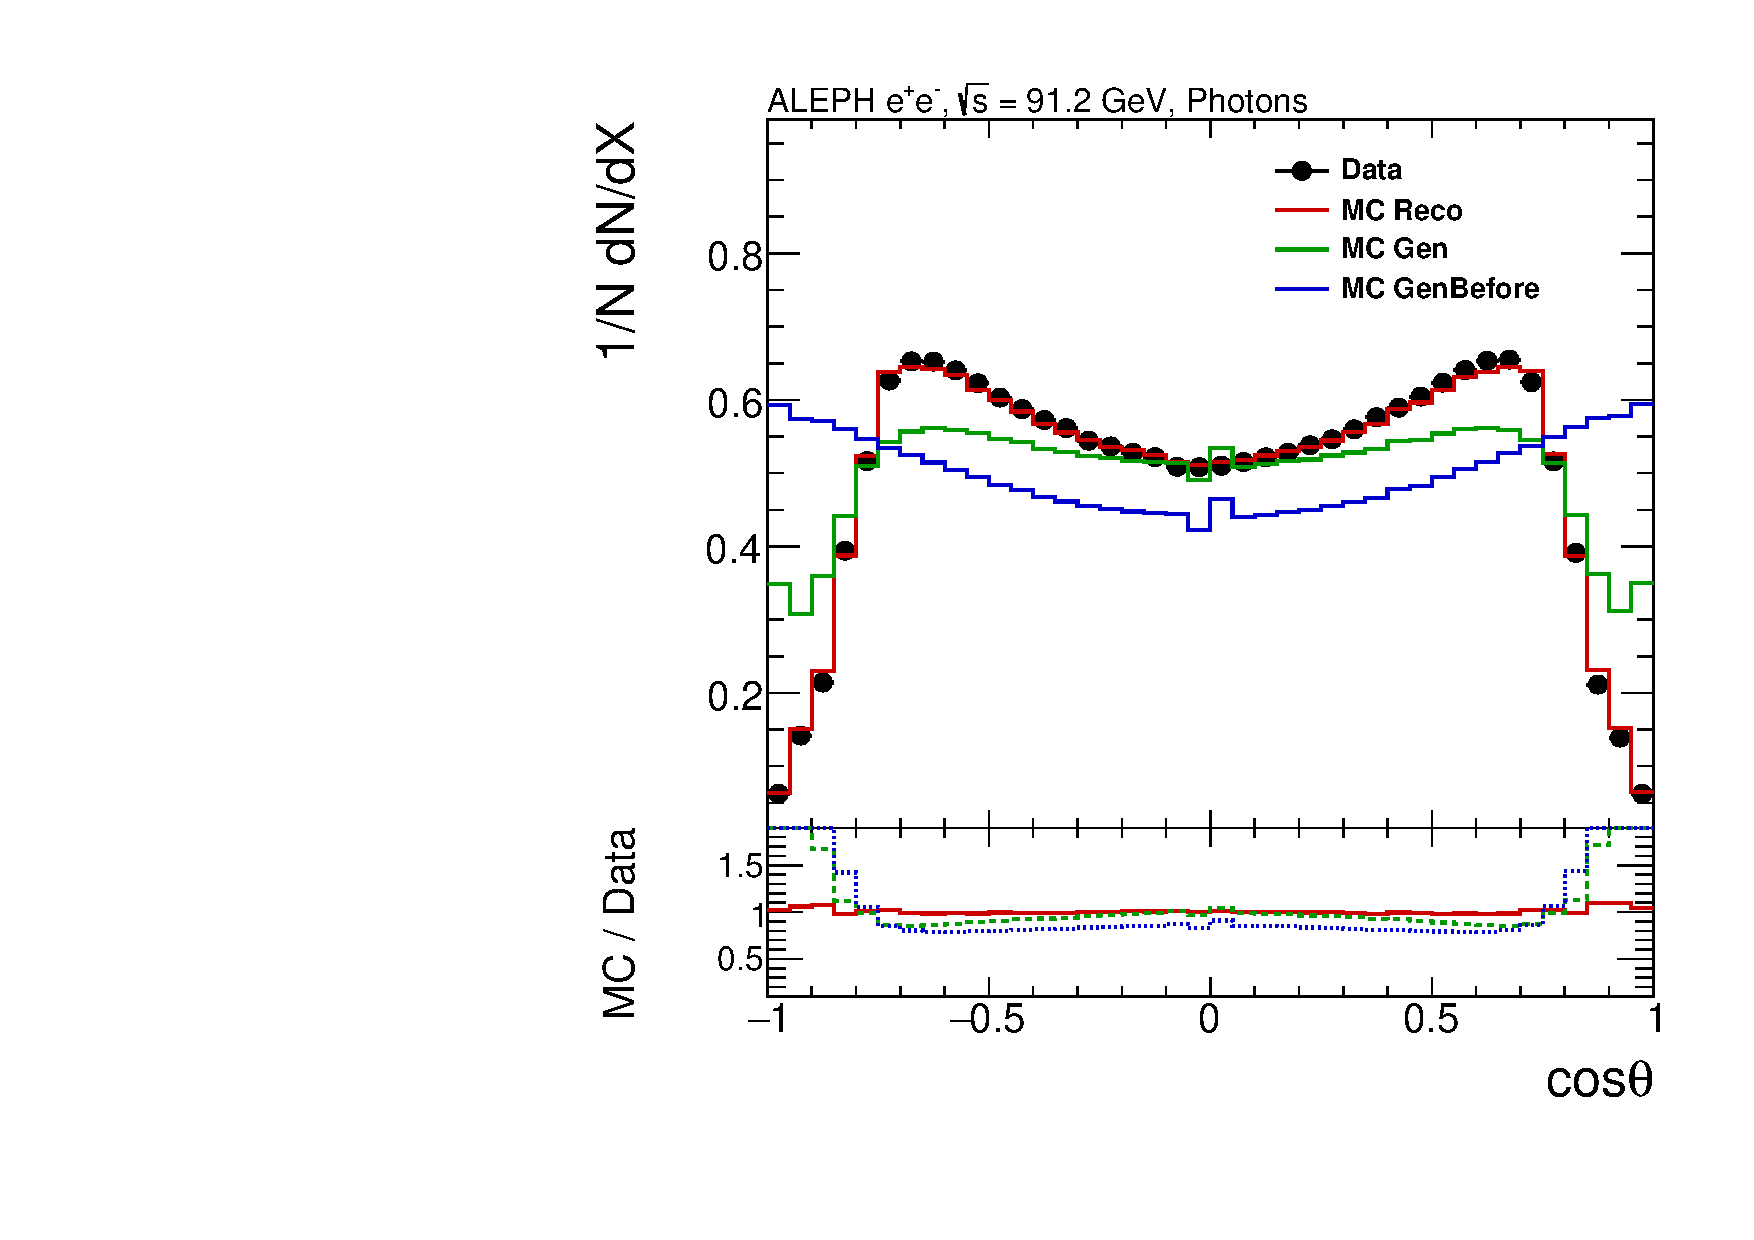
\includegraphics[width=0.325\textwidth]{../Studies/PreliminaryResult/2026-02-17_thrust_iter5/pwflag_kinematics/pwflag4_cosTheta.pdf}
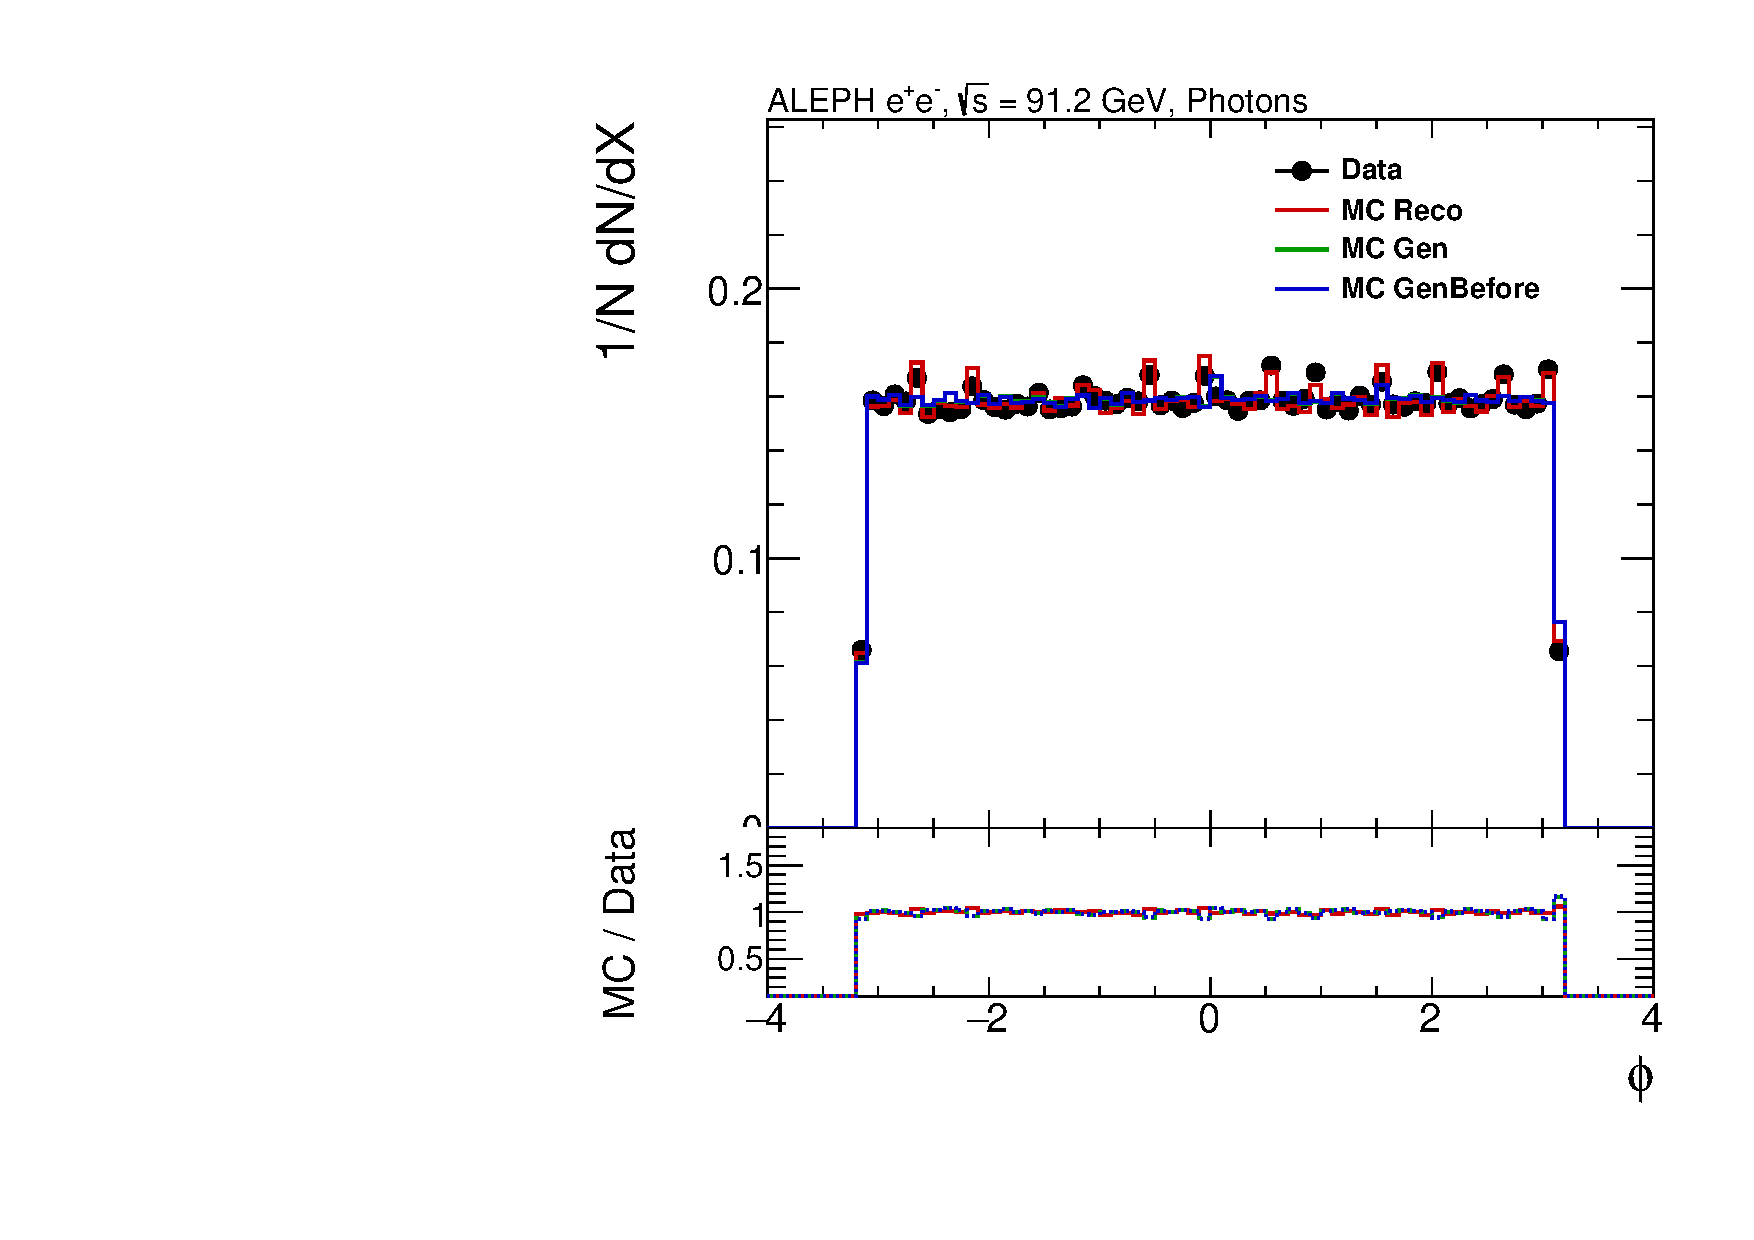
\includegraphics[width=0.325\textwidth]{../Studies/PreliminaryResult/2026-02-17_thrust_iter5/pwflag_kinematics/pwflag4_phi.pdf}
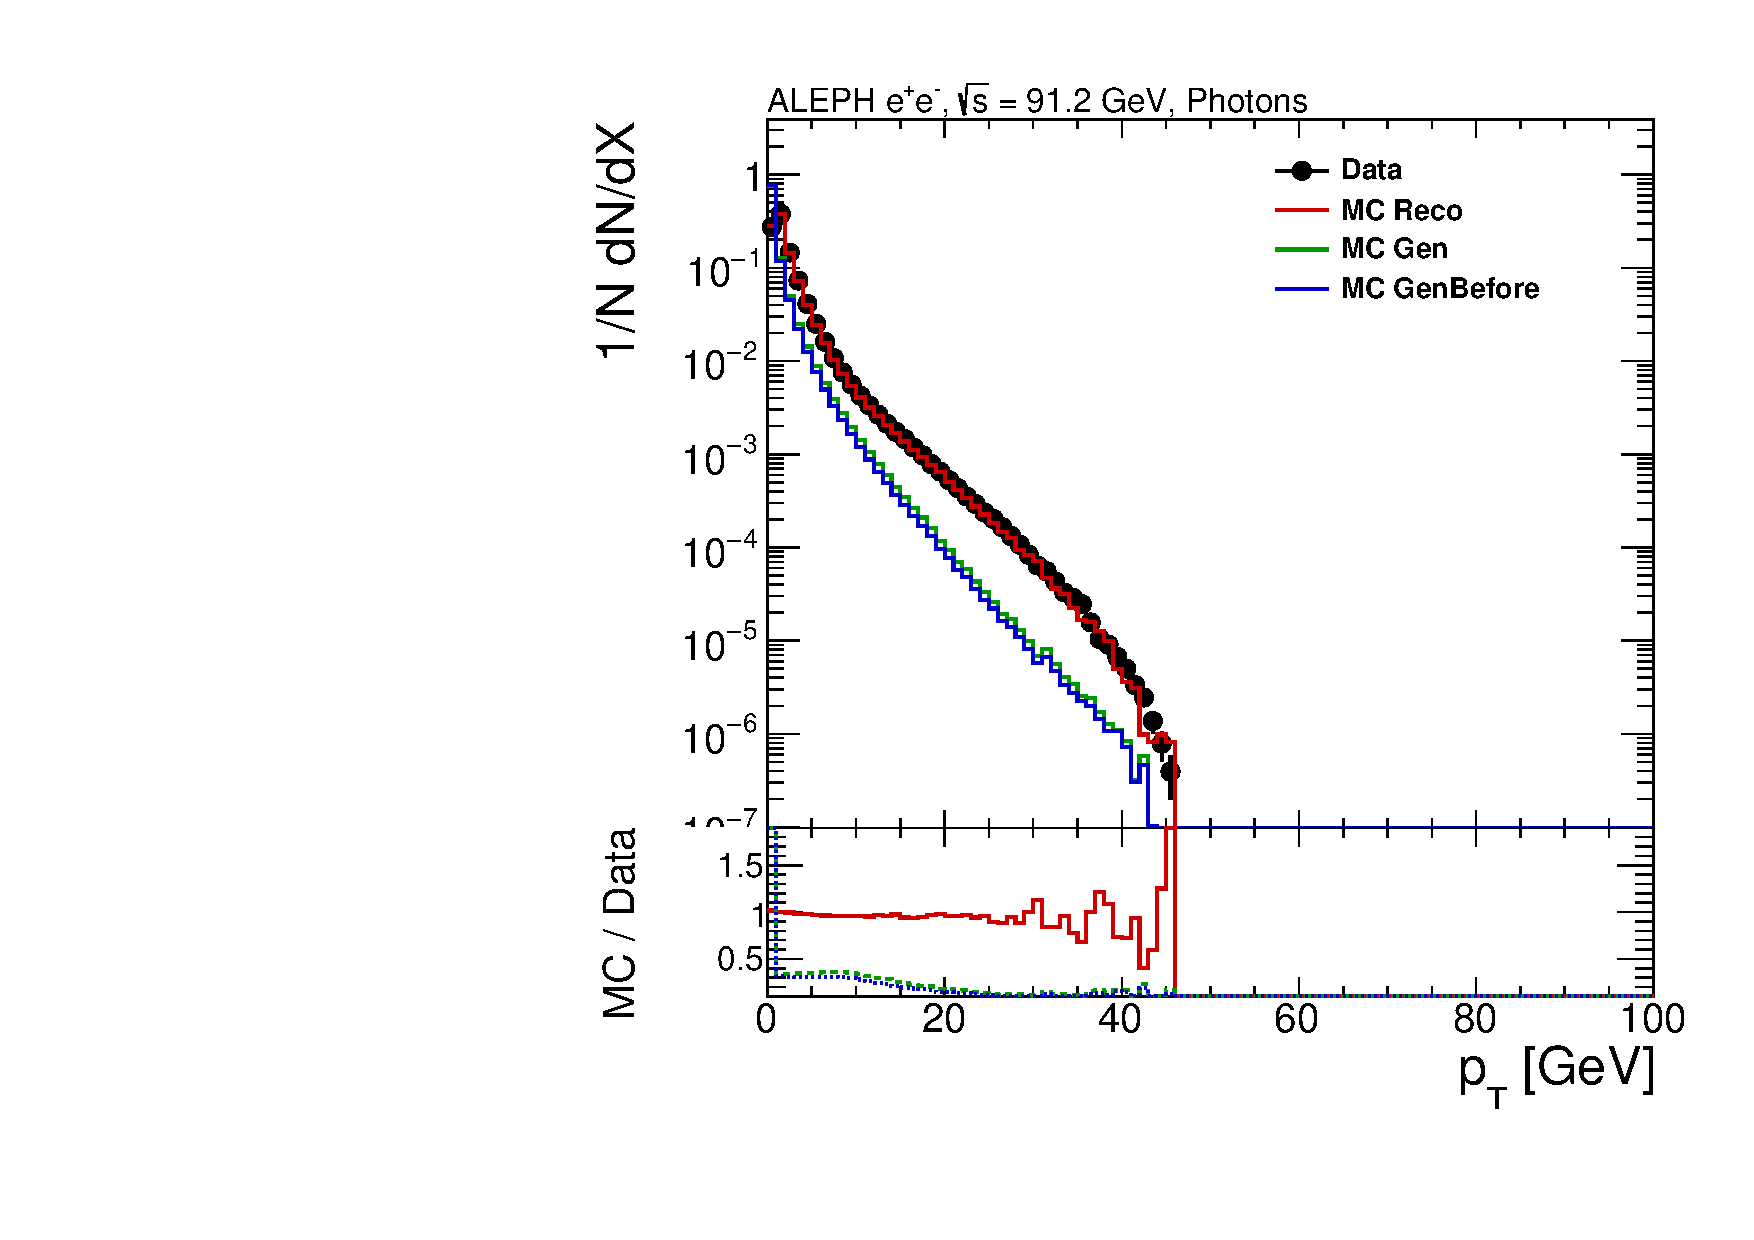
\includegraphics[width=0.325\textwidth]{../Studies/PreliminaryResult/2026-02-17_thrust_iter5/pwflag_kinematics/pwflag4_pt.pdf}
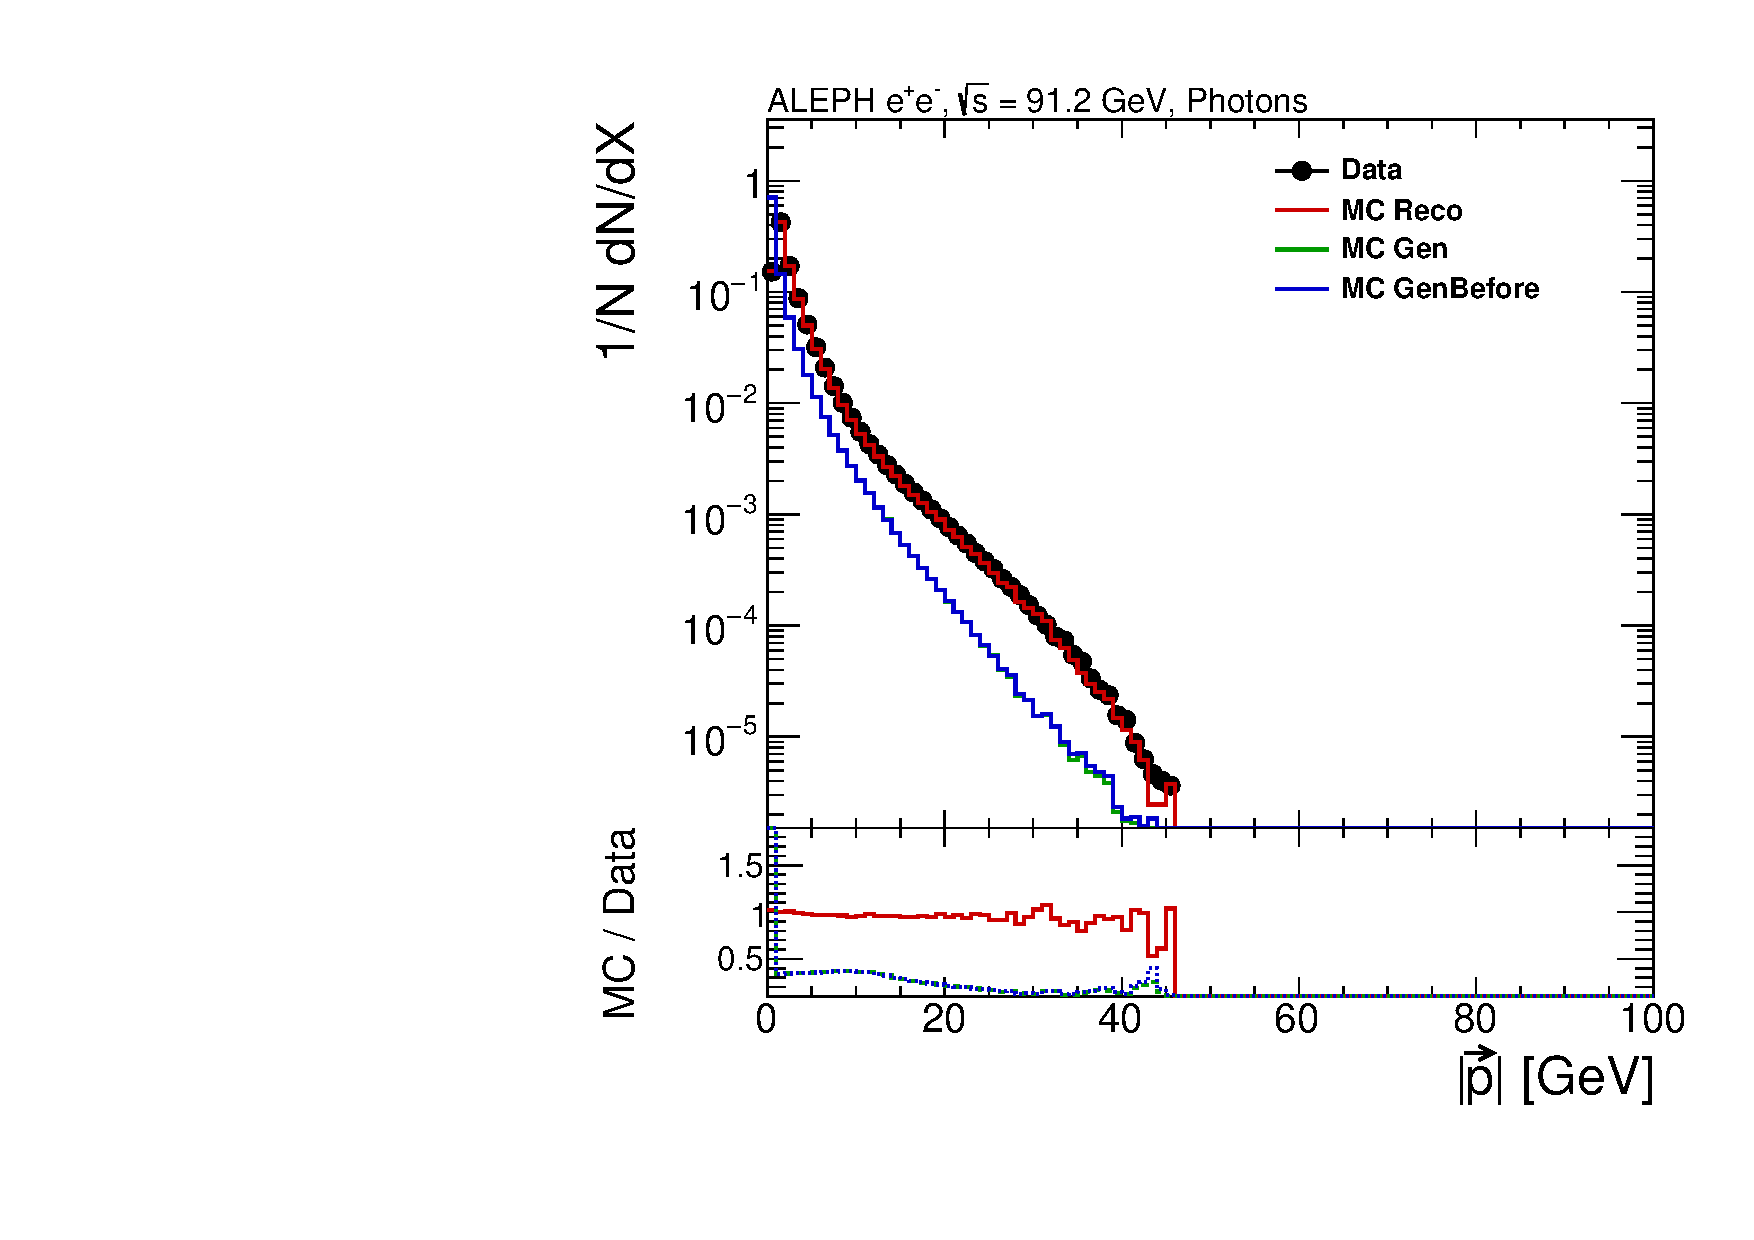
\includegraphics[width=0.325\textwidth]{../Studies/PreliminaryResult/2026-02-17_thrust_iter5/pwflag_kinematics/pwflag4_pmag.pdf}
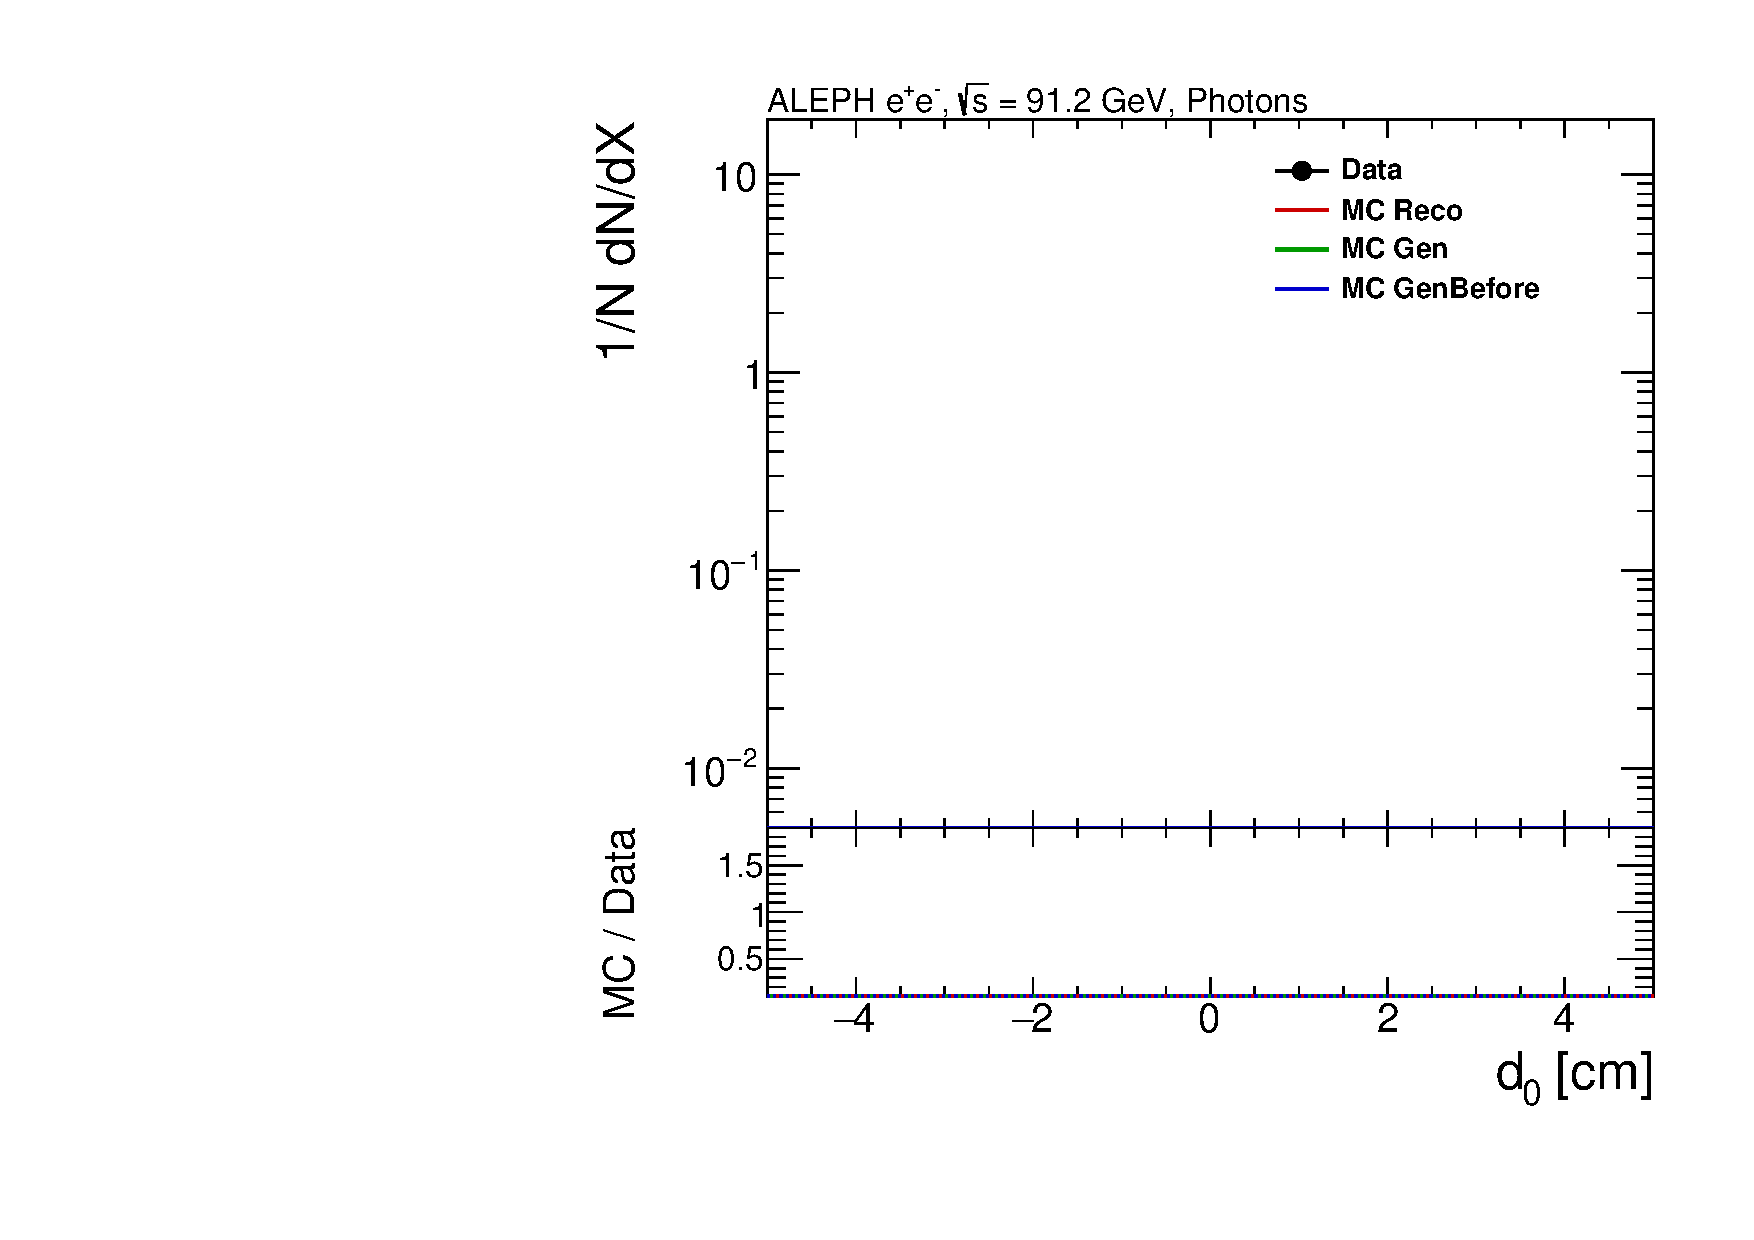
\includegraphics[width=0.325\textwidth]{../Studies/PreliminaryResult/2026-02-17_thrust_iter5/pwflag_kinematics/pwflag4_d0.pdf}
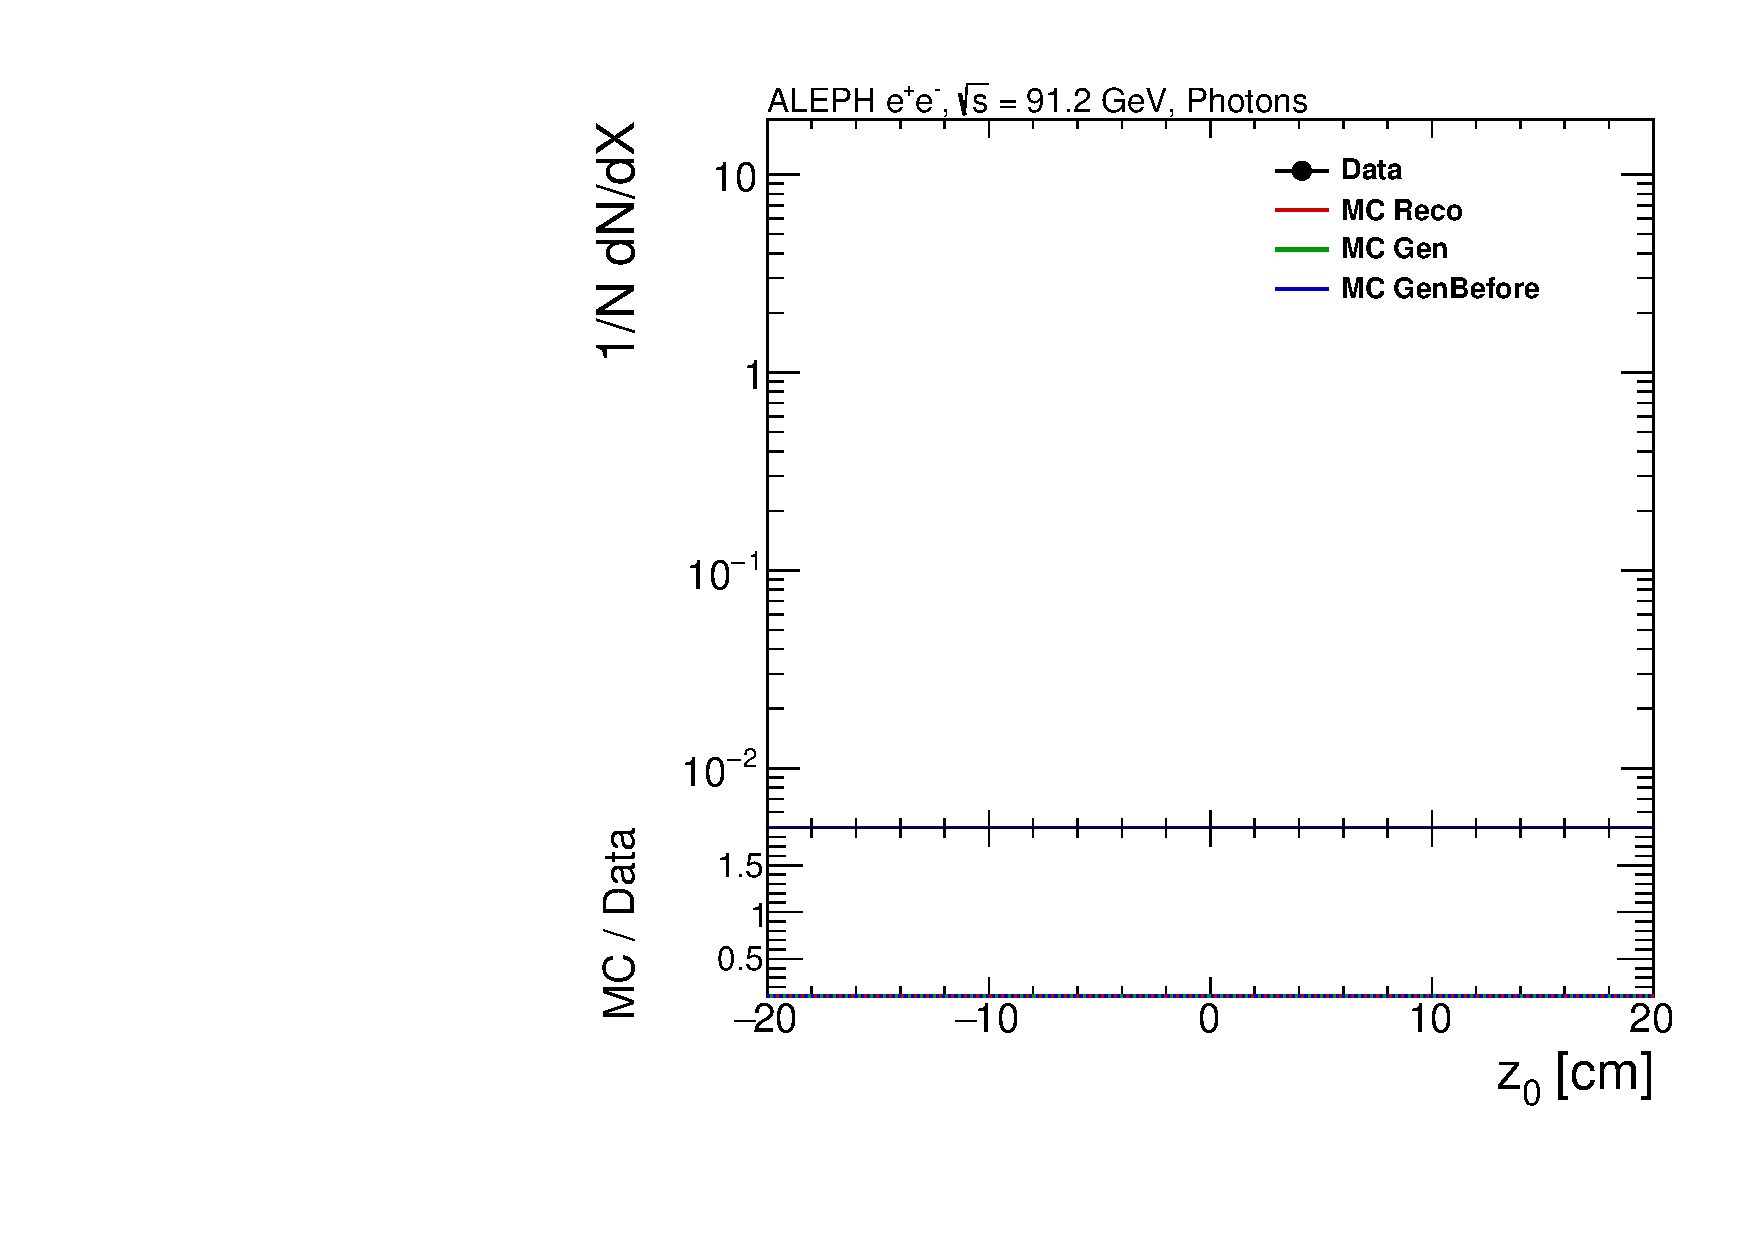
\includegraphics[width=0.325\textwidth]{../Studies/PreliminaryResult/2026-02-17_thrust_iter5/pwflag_kinematics/pwflag4_z0.pdf}
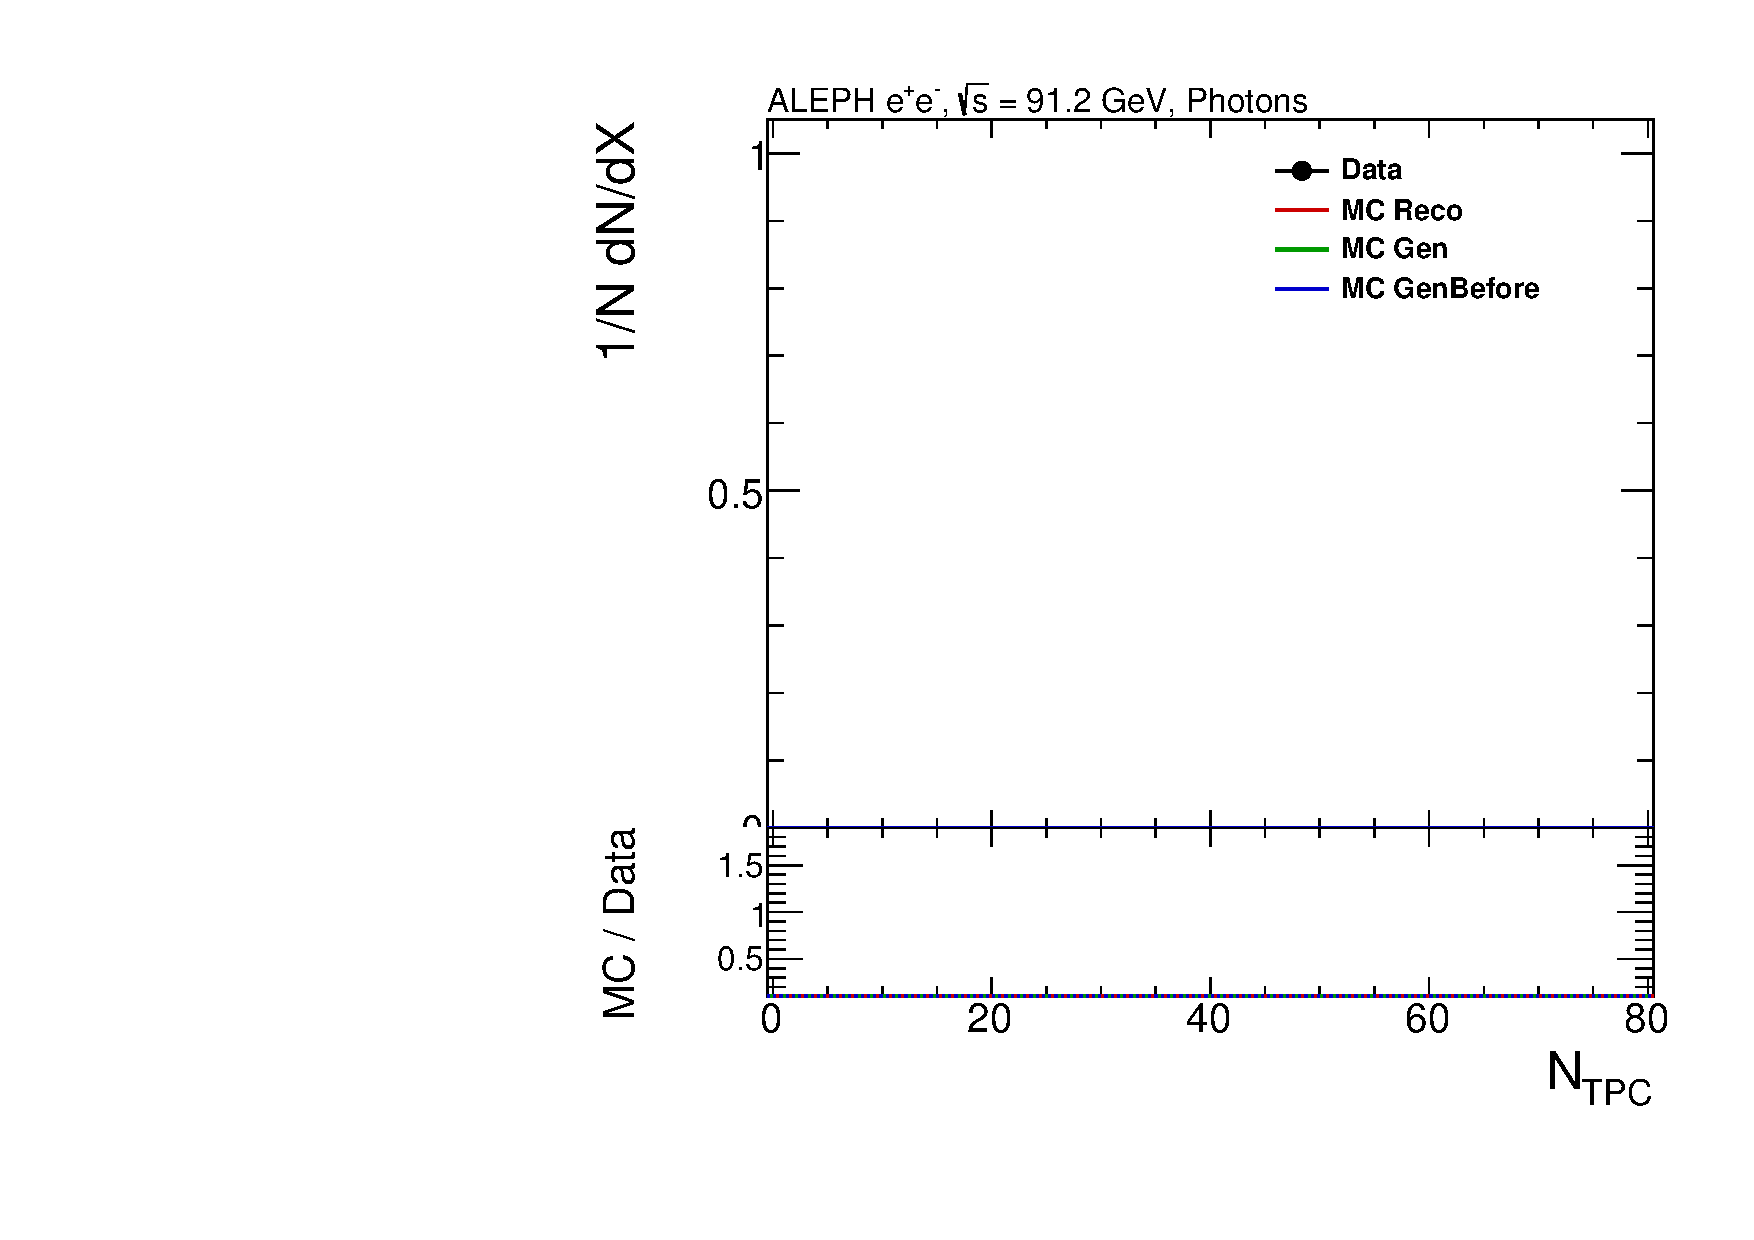
\includegraphics[width=0.325\textwidth]{../Studies/PreliminaryResult/2026-02-17_thrust_iter5/pwflag_kinematics/pwflag4_ntpc.pdf}
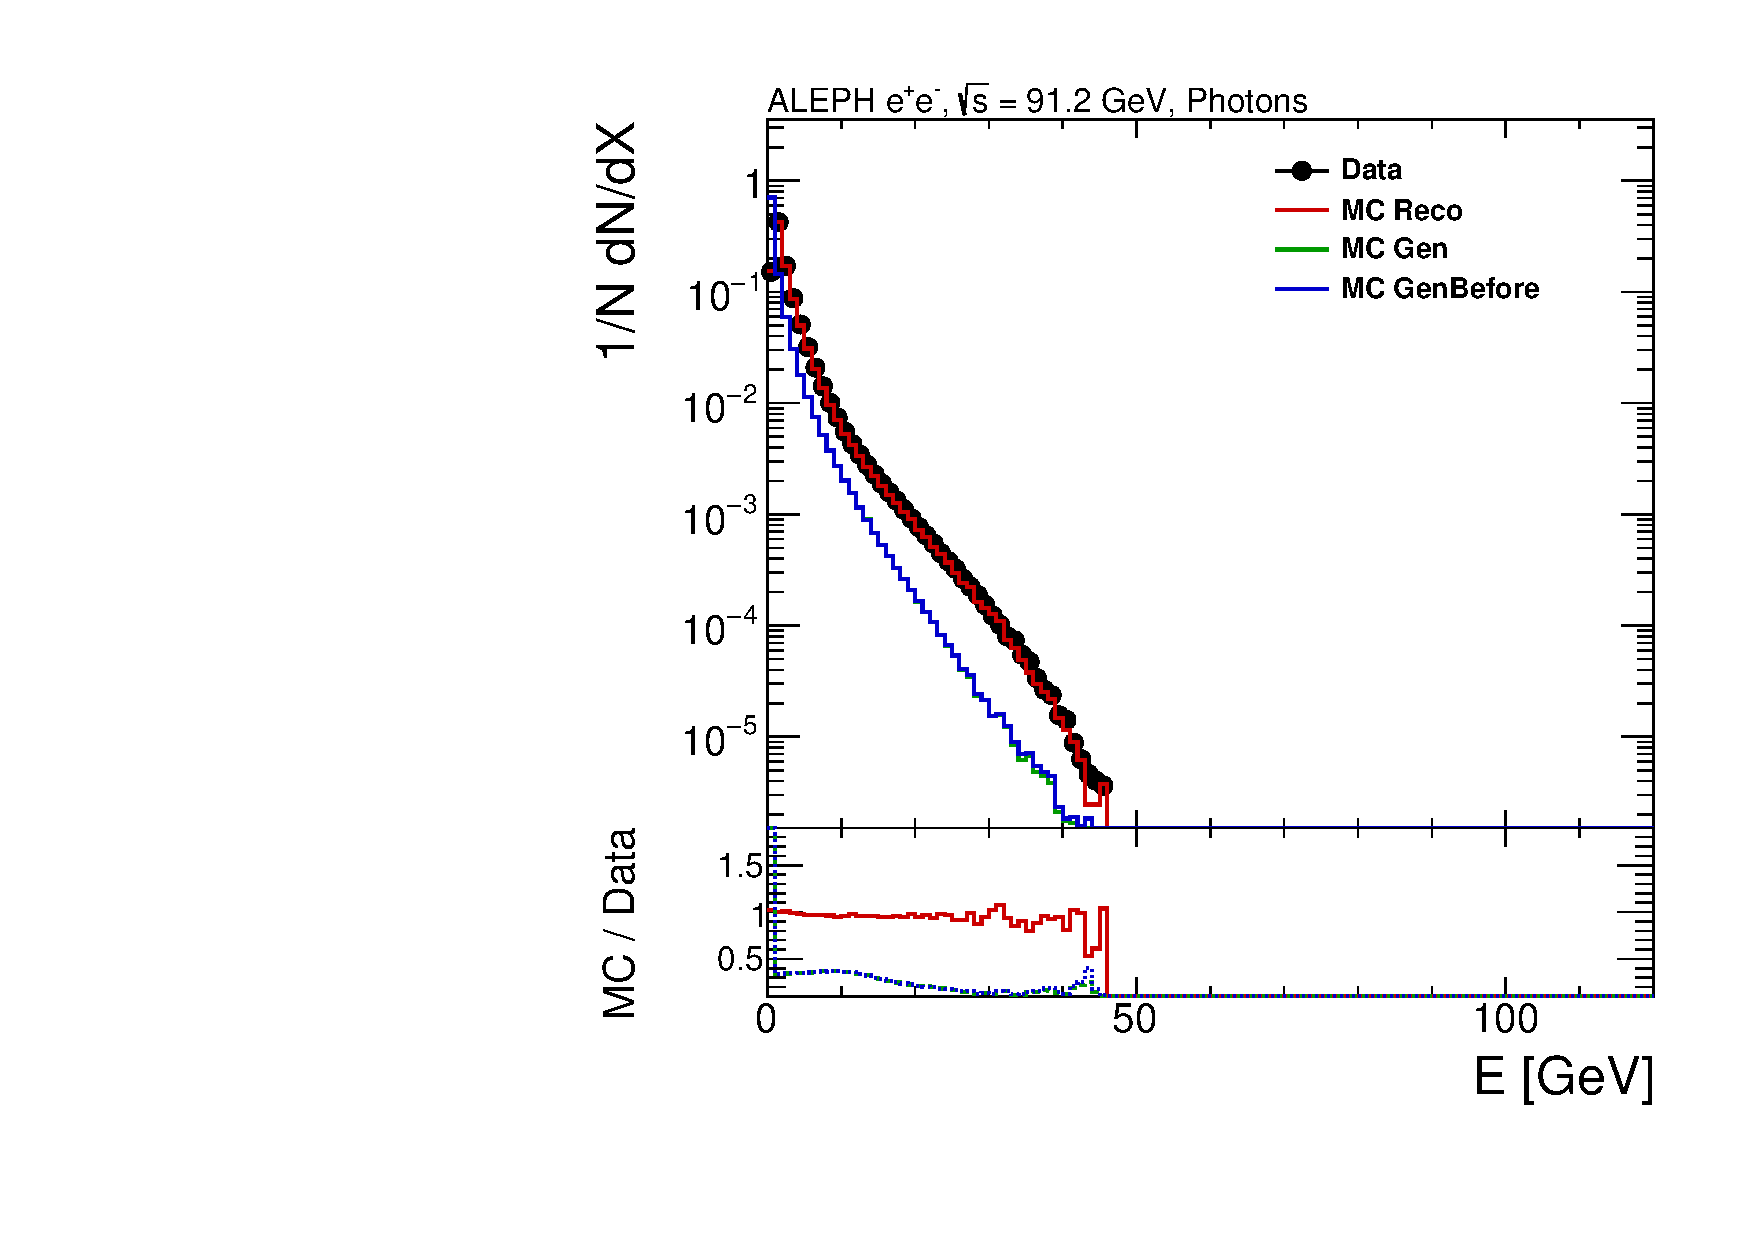
\includegraphics[width=0.325\textwidth]{../Studies/PreliminaryResult/2026-02-17_thrust_iter5/pwflag_kinematics/pwflag4_energy.pdf}
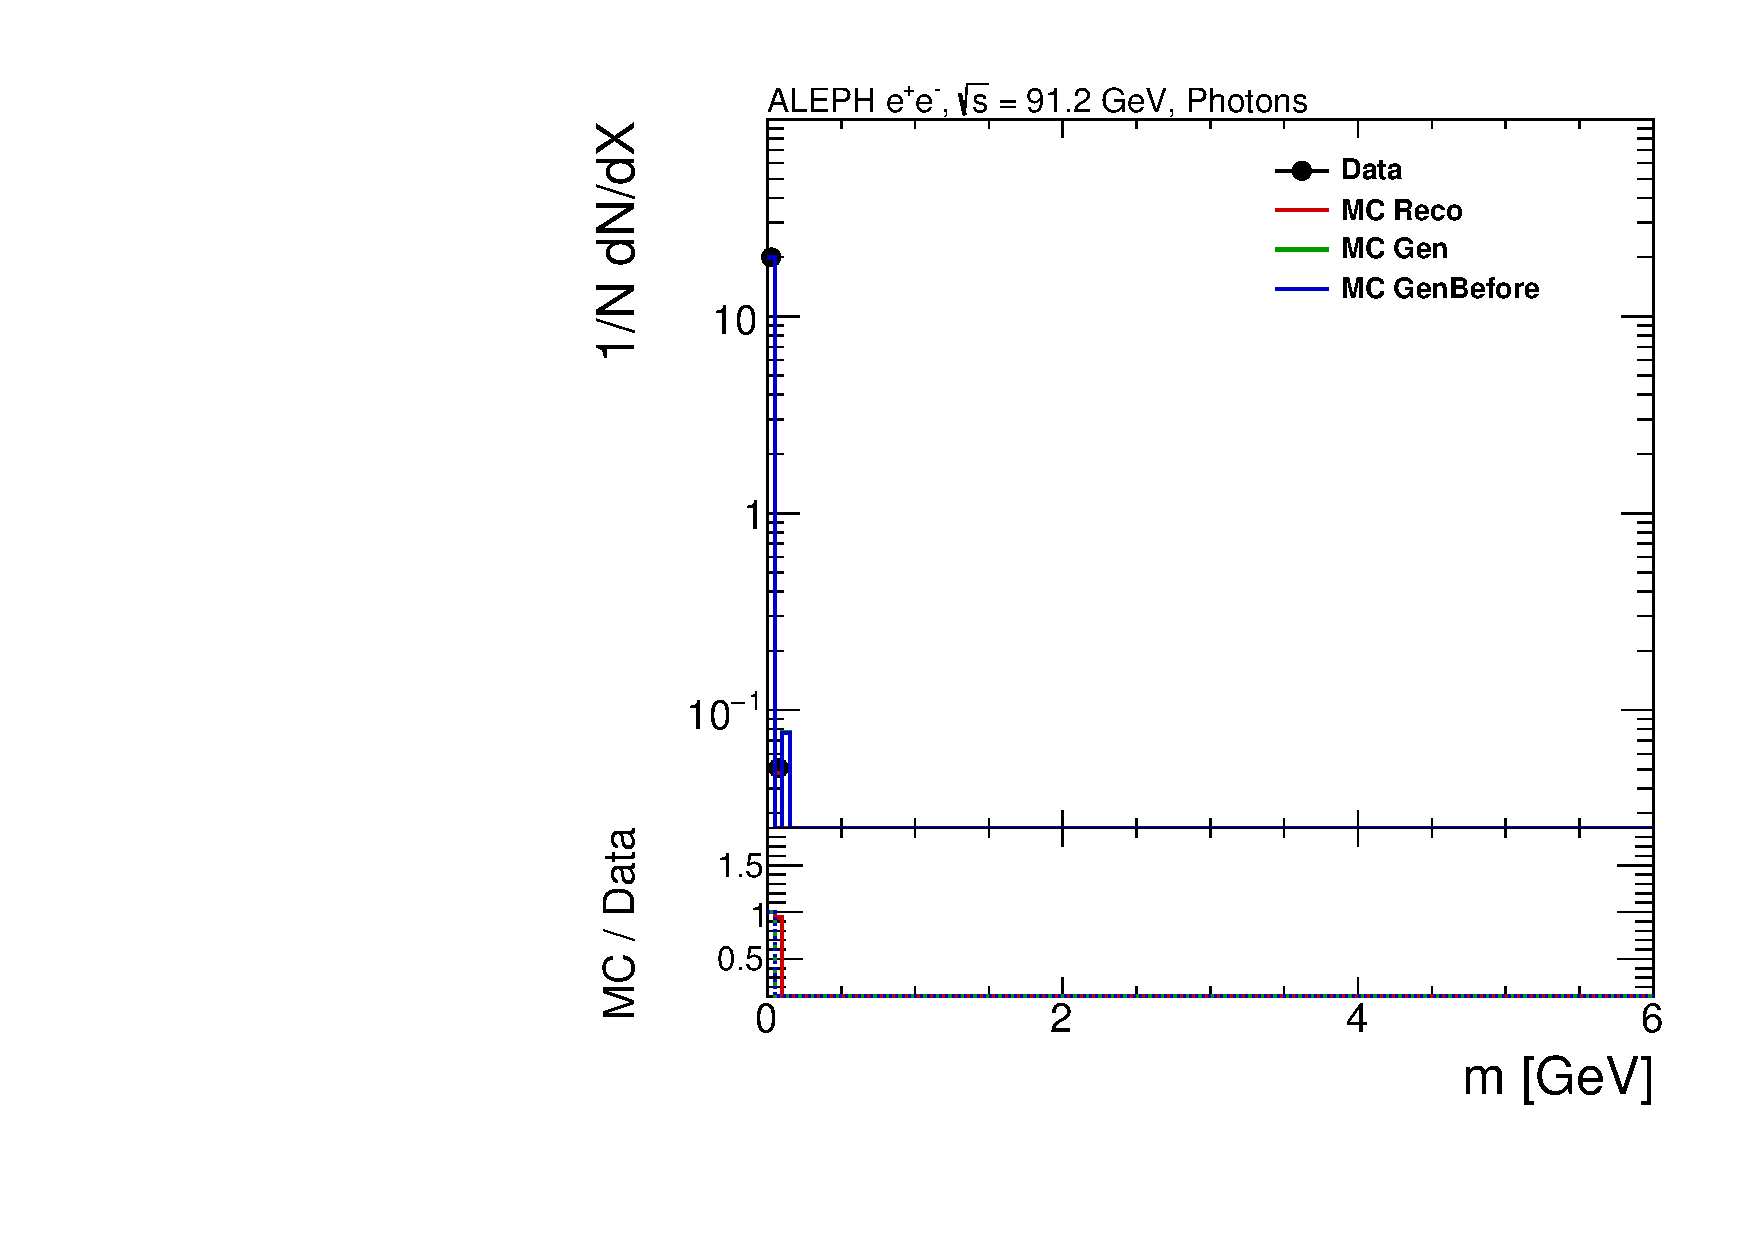
\includegraphics[width=0.325\textwidth]{../Studies/PreliminaryResult/2026-02-17_thrust_iter5/pwflag_kinematics/pwflag4_mass.pdf}
\caption{Complete \texttt{pwflag}=4 kinematic set.}
\label{fig:pwflag4_full}
\end{figure}

\noindent
Figure~\ref{fig:pwflag4_full} isolates photons, which probe neutral electromagnetic response and
its effect on event-shape normalization. The photon energy and angular spectra are especially
important because electromagnetic neutral energy contributes directly to visible event topology and
hemisphere energy balance. The observed data/MC consistency in the core region supports the
neutral-energy calibration assumptions used in the nominal unfolding and neutral-response
systematic variations.

\begin{figure}[t!]
\centering
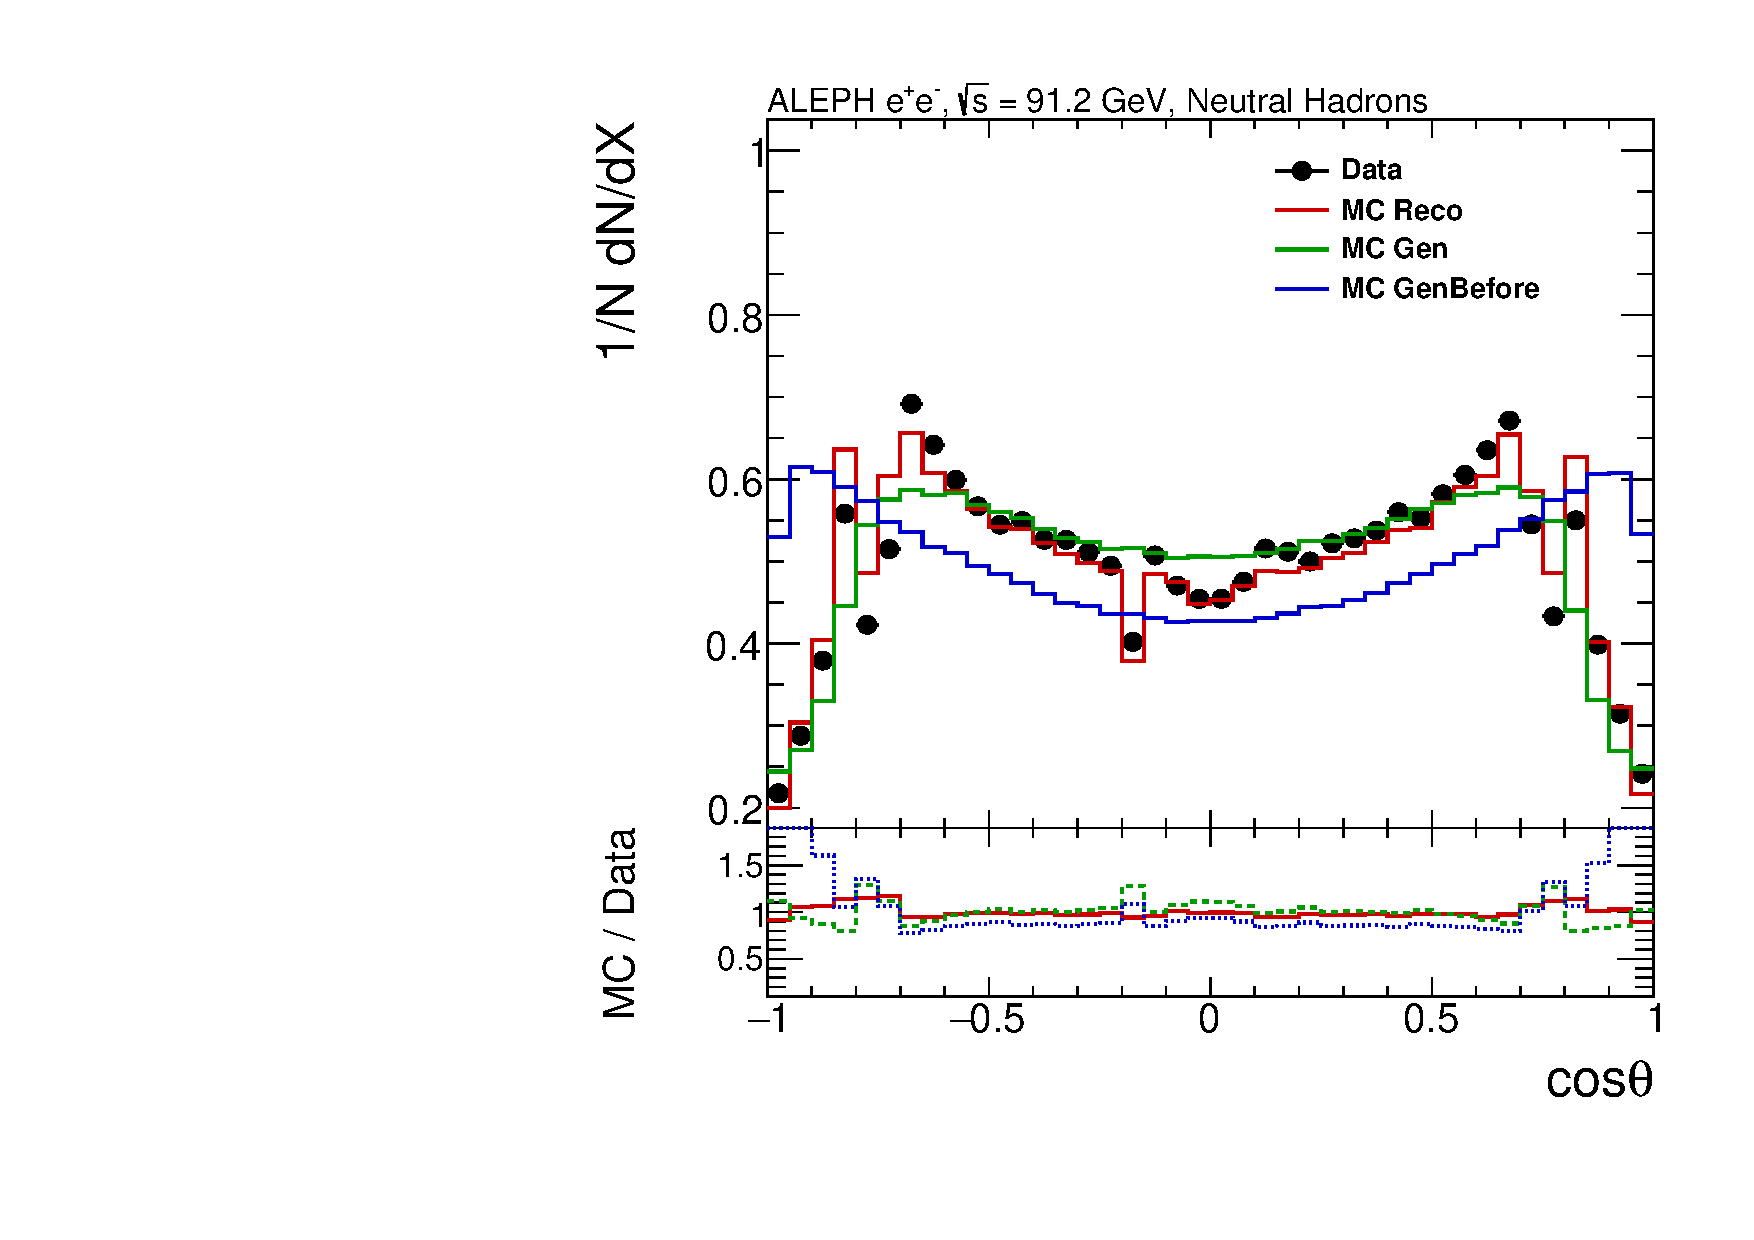
\includegraphics[width=0.325\textwidth]{../Studies/PreliminaryResult/2026-02-17_thrust_iter5/pwflag_kinematics/pwflag5_cosTheta.pdf}
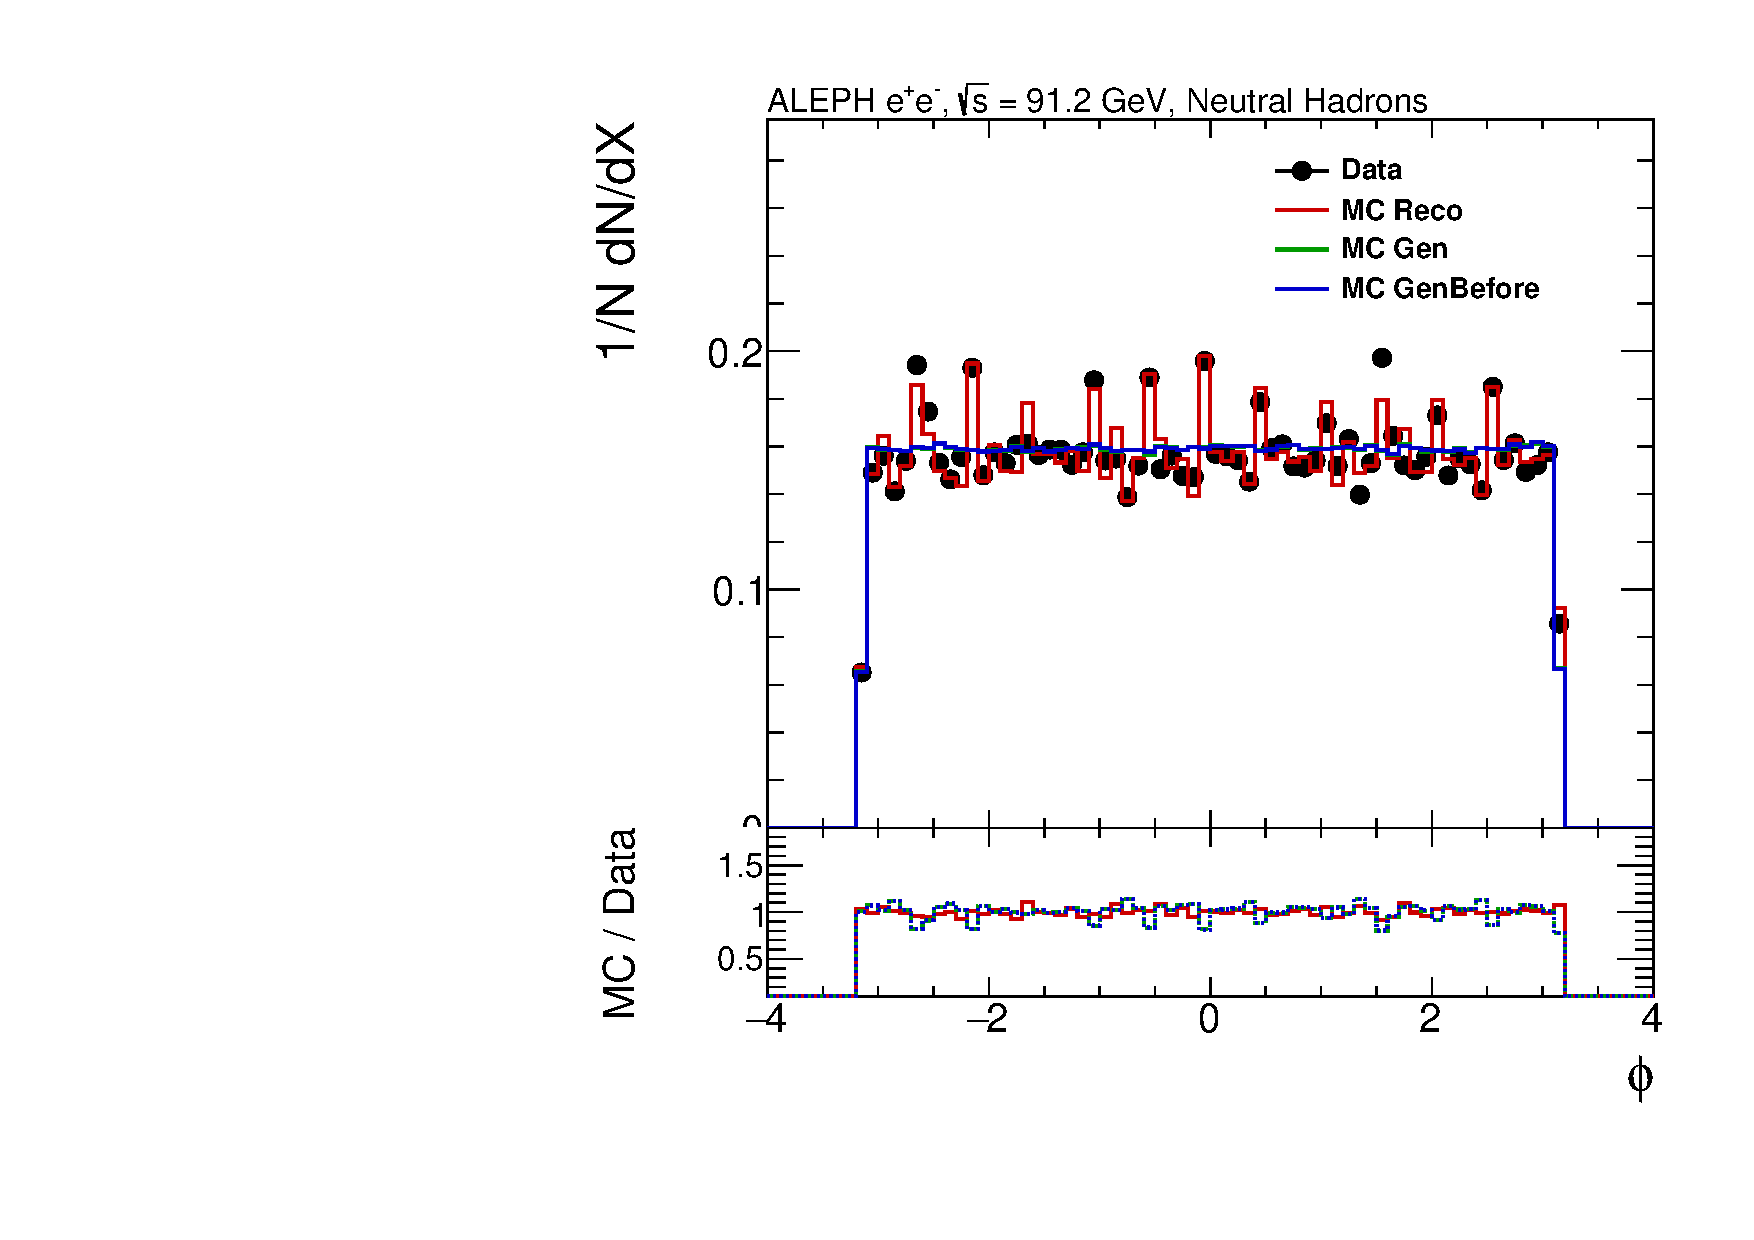
\includegraphics[width=0.325\textwidth]{../Studies/PreliminaryResult/2026-02-17_thrust_iter5/pwflag_kinematics/pwflag5_phi.pdf}
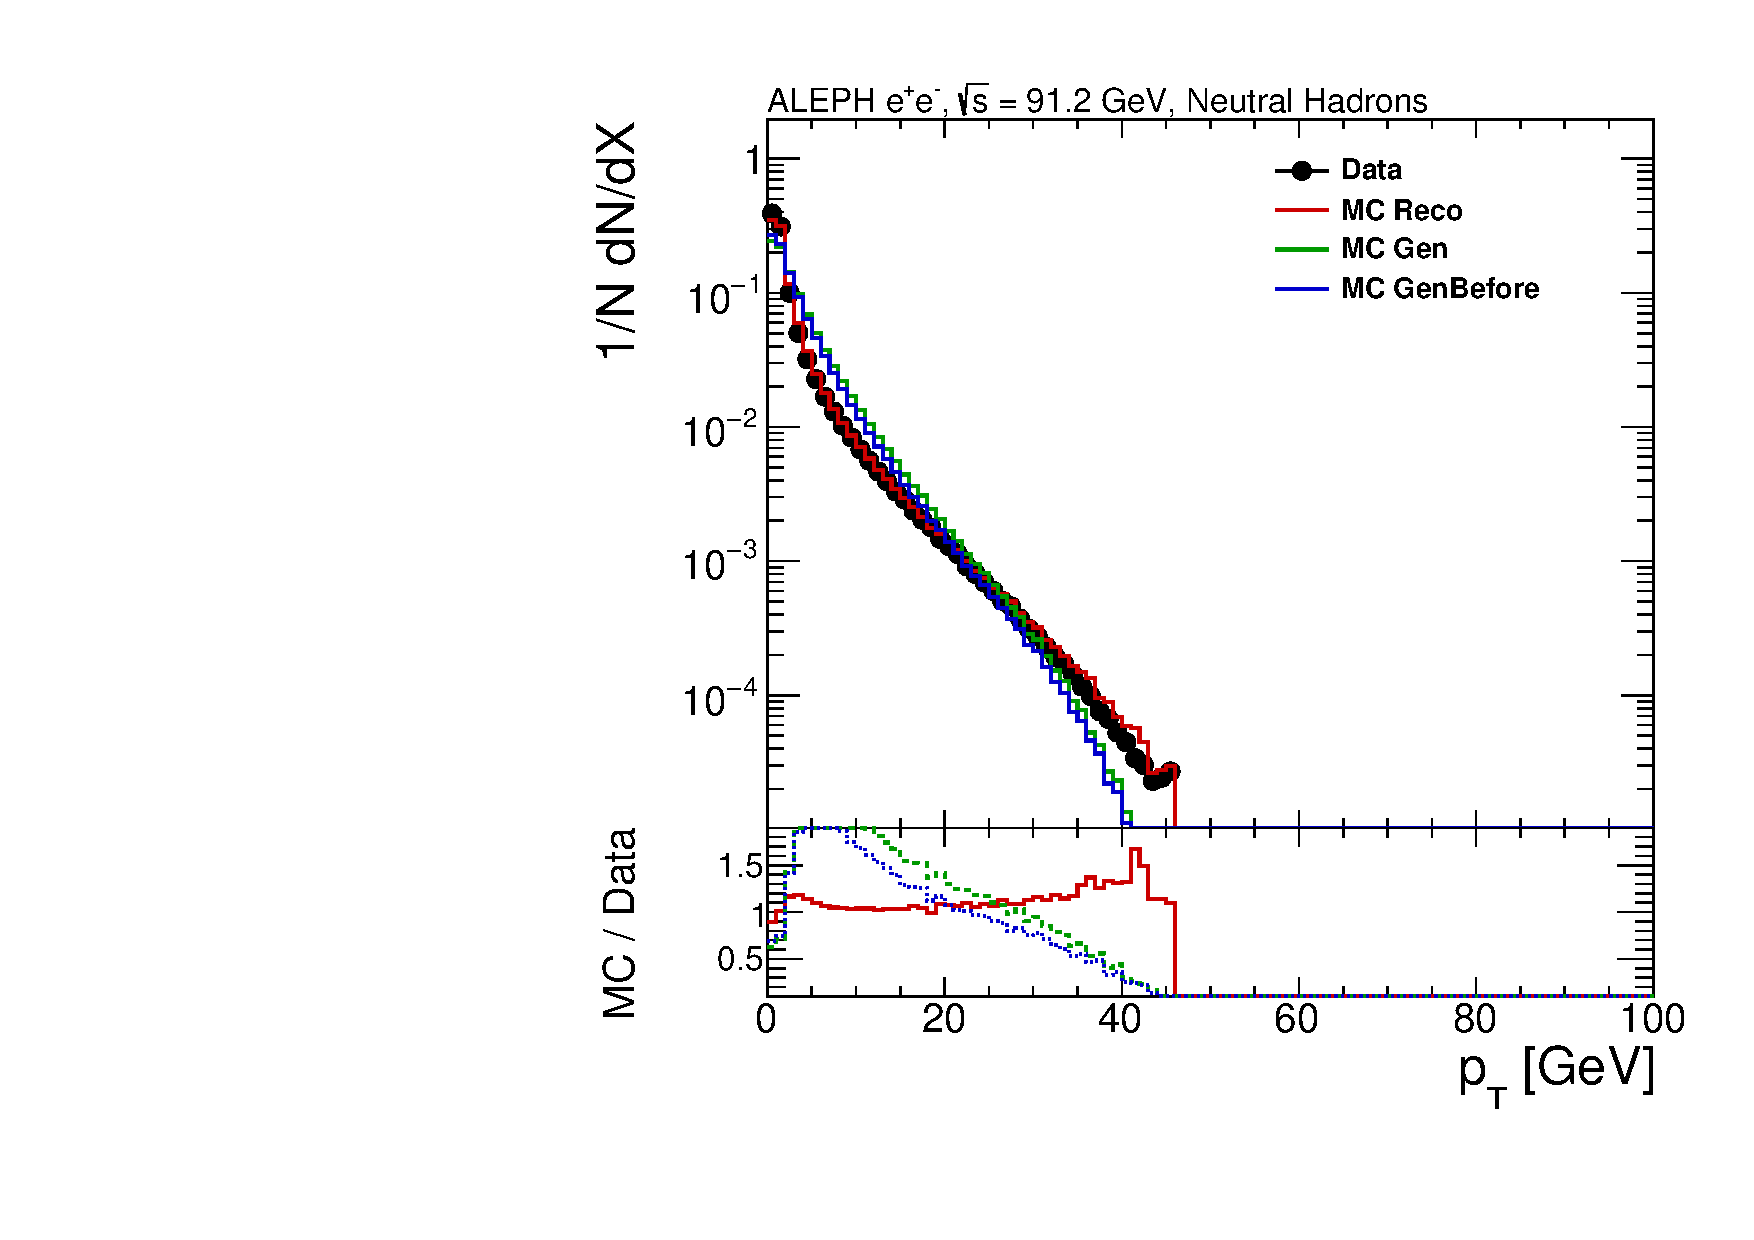
\includegraphics[width=0.325\textwidth]{../Studies/PreliminaryResult/2026-02-17_thrust_iter5/pwflag_kinematics/pwflag5_pt.pdf}
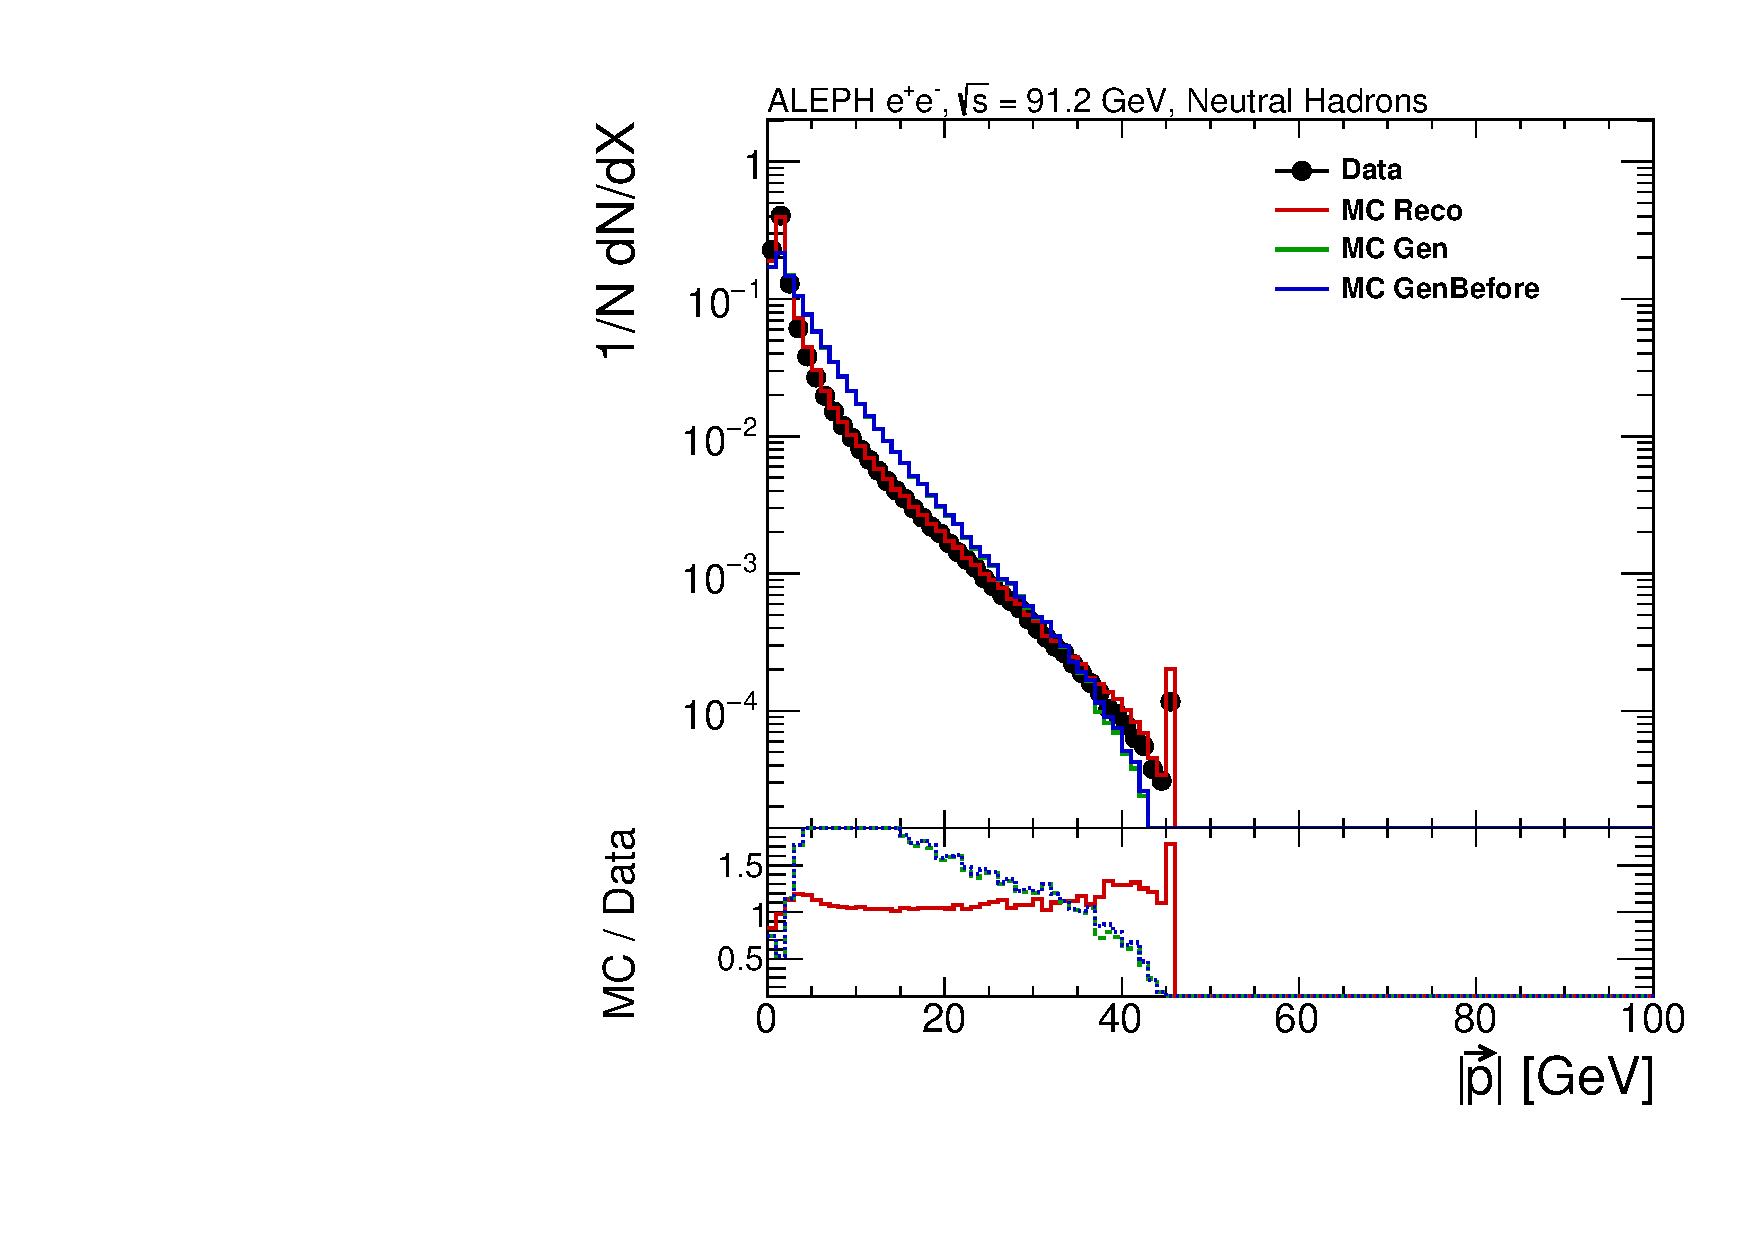
\includegraphics[width=0.325\textwidth]{../Studies/PreliminaryResult/2026-02-17_thrust_iter5/pwflag_kinematics/pwflag5_pmag.pdf}
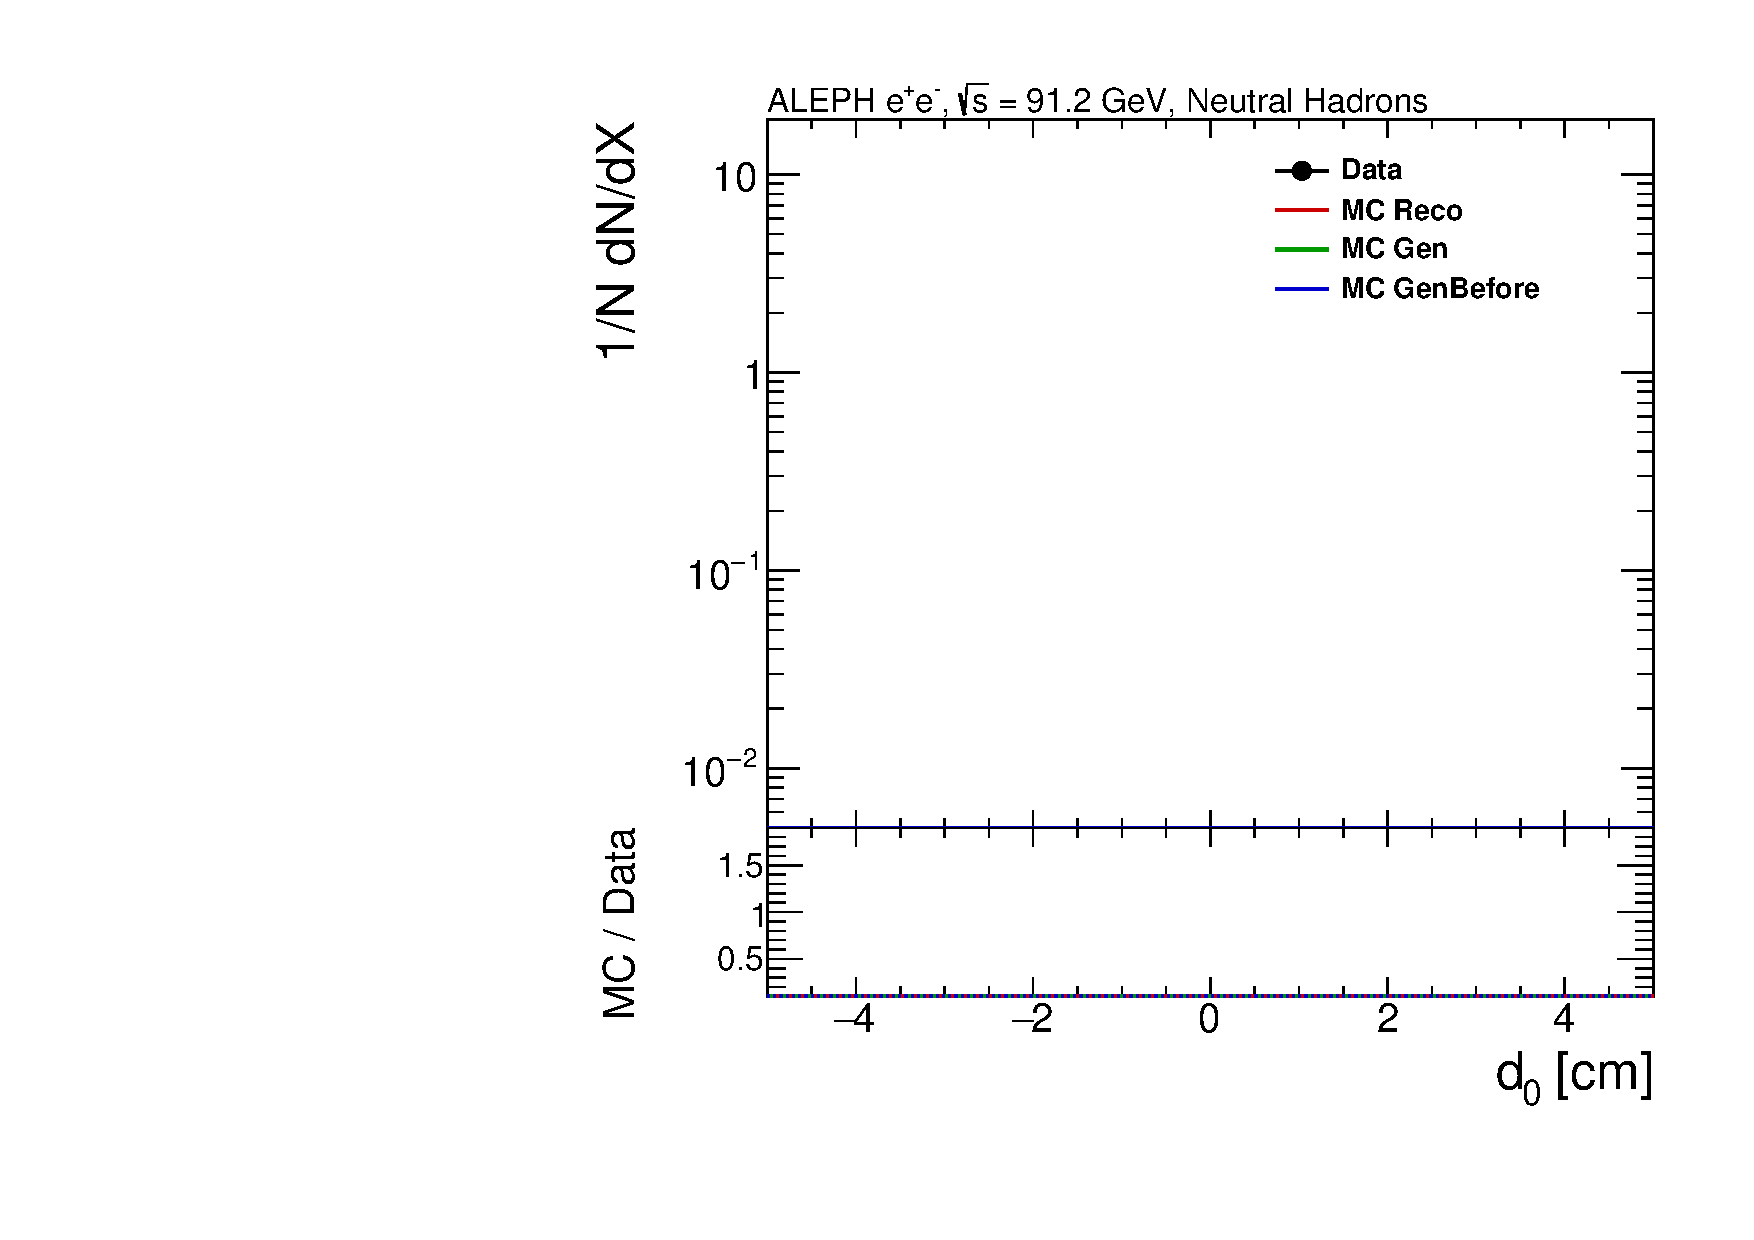
\includegraphics[width=0.325\textwidth]{../Studies/PreliminaryResult/2026-02-17_thrust_iter5/pwflag_kinematics/pwflag5_d0.pdf}
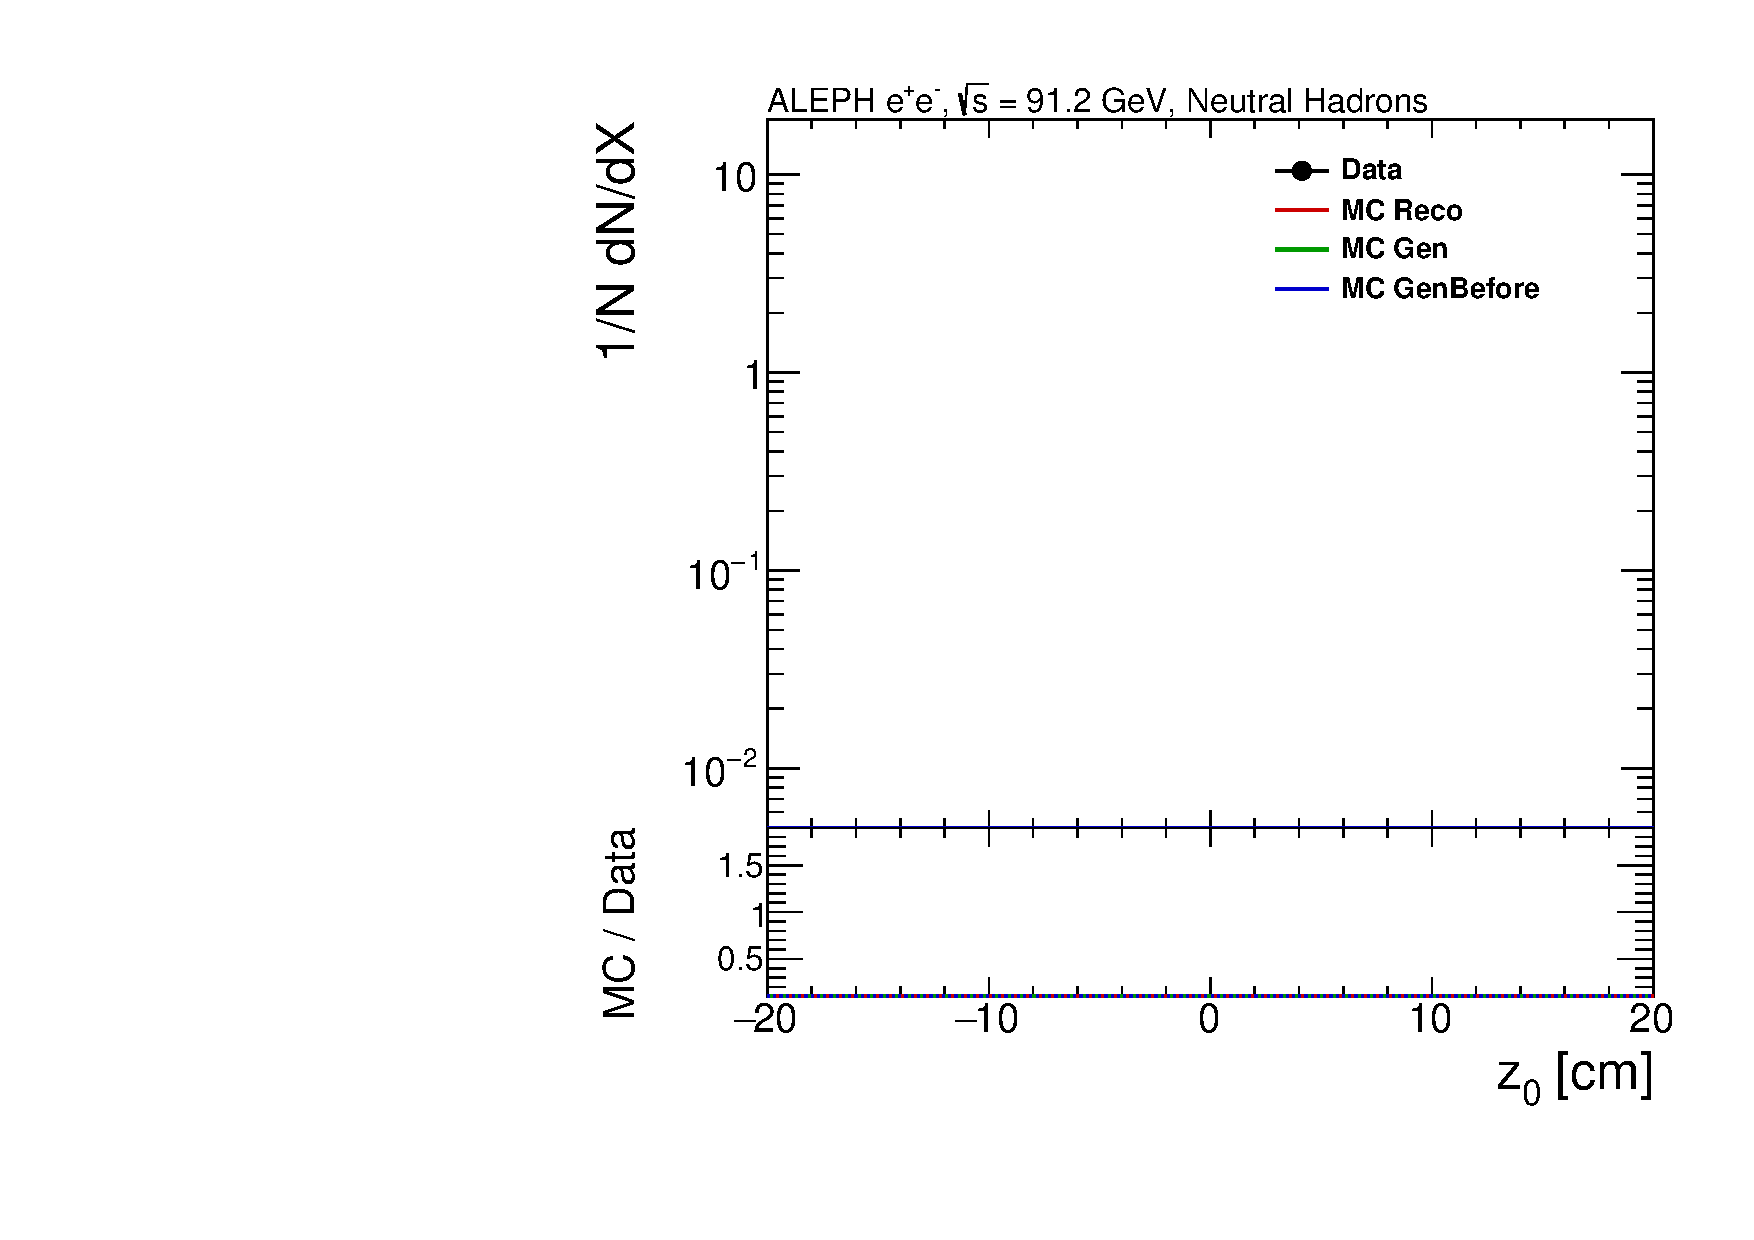
\includegraphics[width=0.325\textwidth]{../Studies/PreliminaryResult/2026-02-17_thrust_iter5/pwflag_kinematics/pwflag5_z0.pdf}
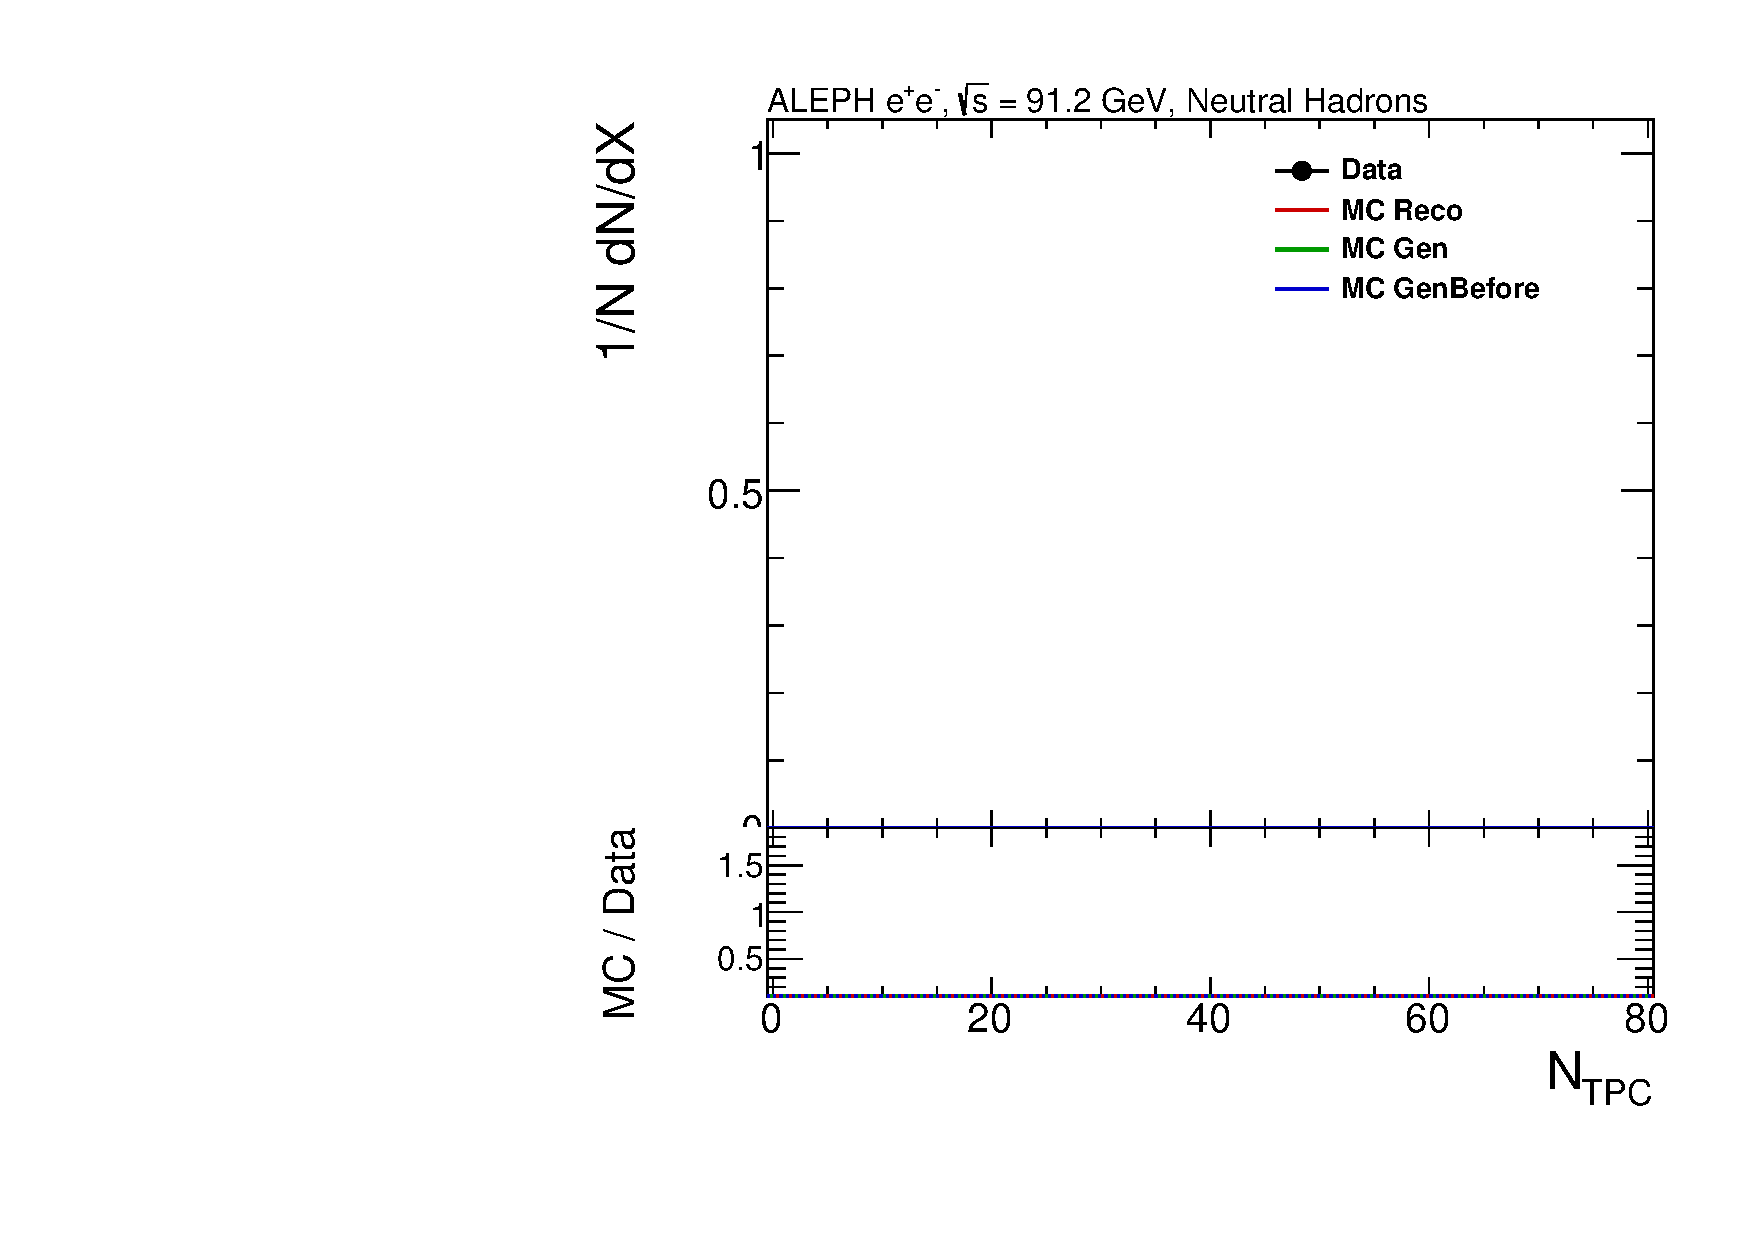
\includegraphics[width=0.325\textwidth]{../Studies/PreliminaryResult/2026-02-17_thrust_iter5/pwflag_kinematics/pwflag5_ntpc.pdf}
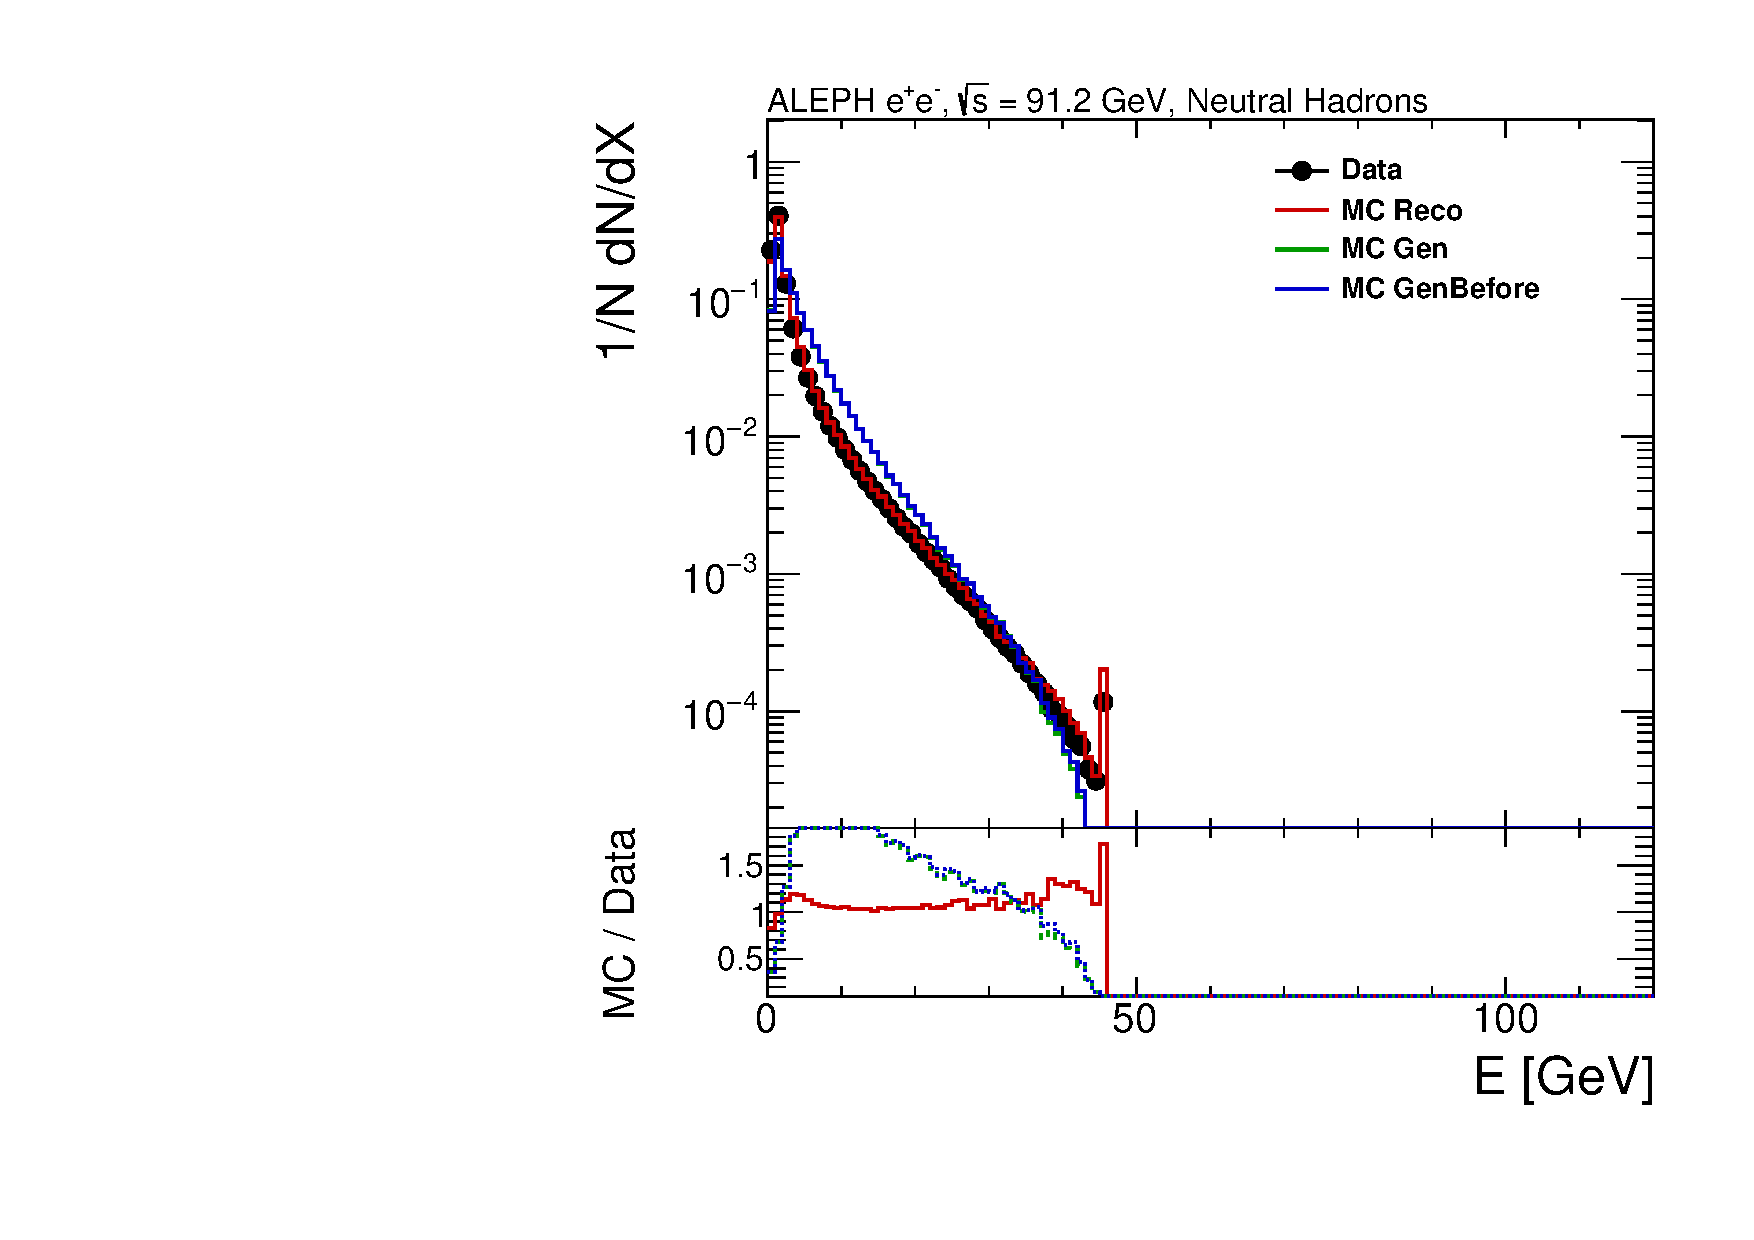
\includegraphics[width=0.325\textwidth]{../Studies/PreliminaryResult/2026-02-17_thrust_iter5/pwflag_kinematics/pwflag5_energy.pdf}
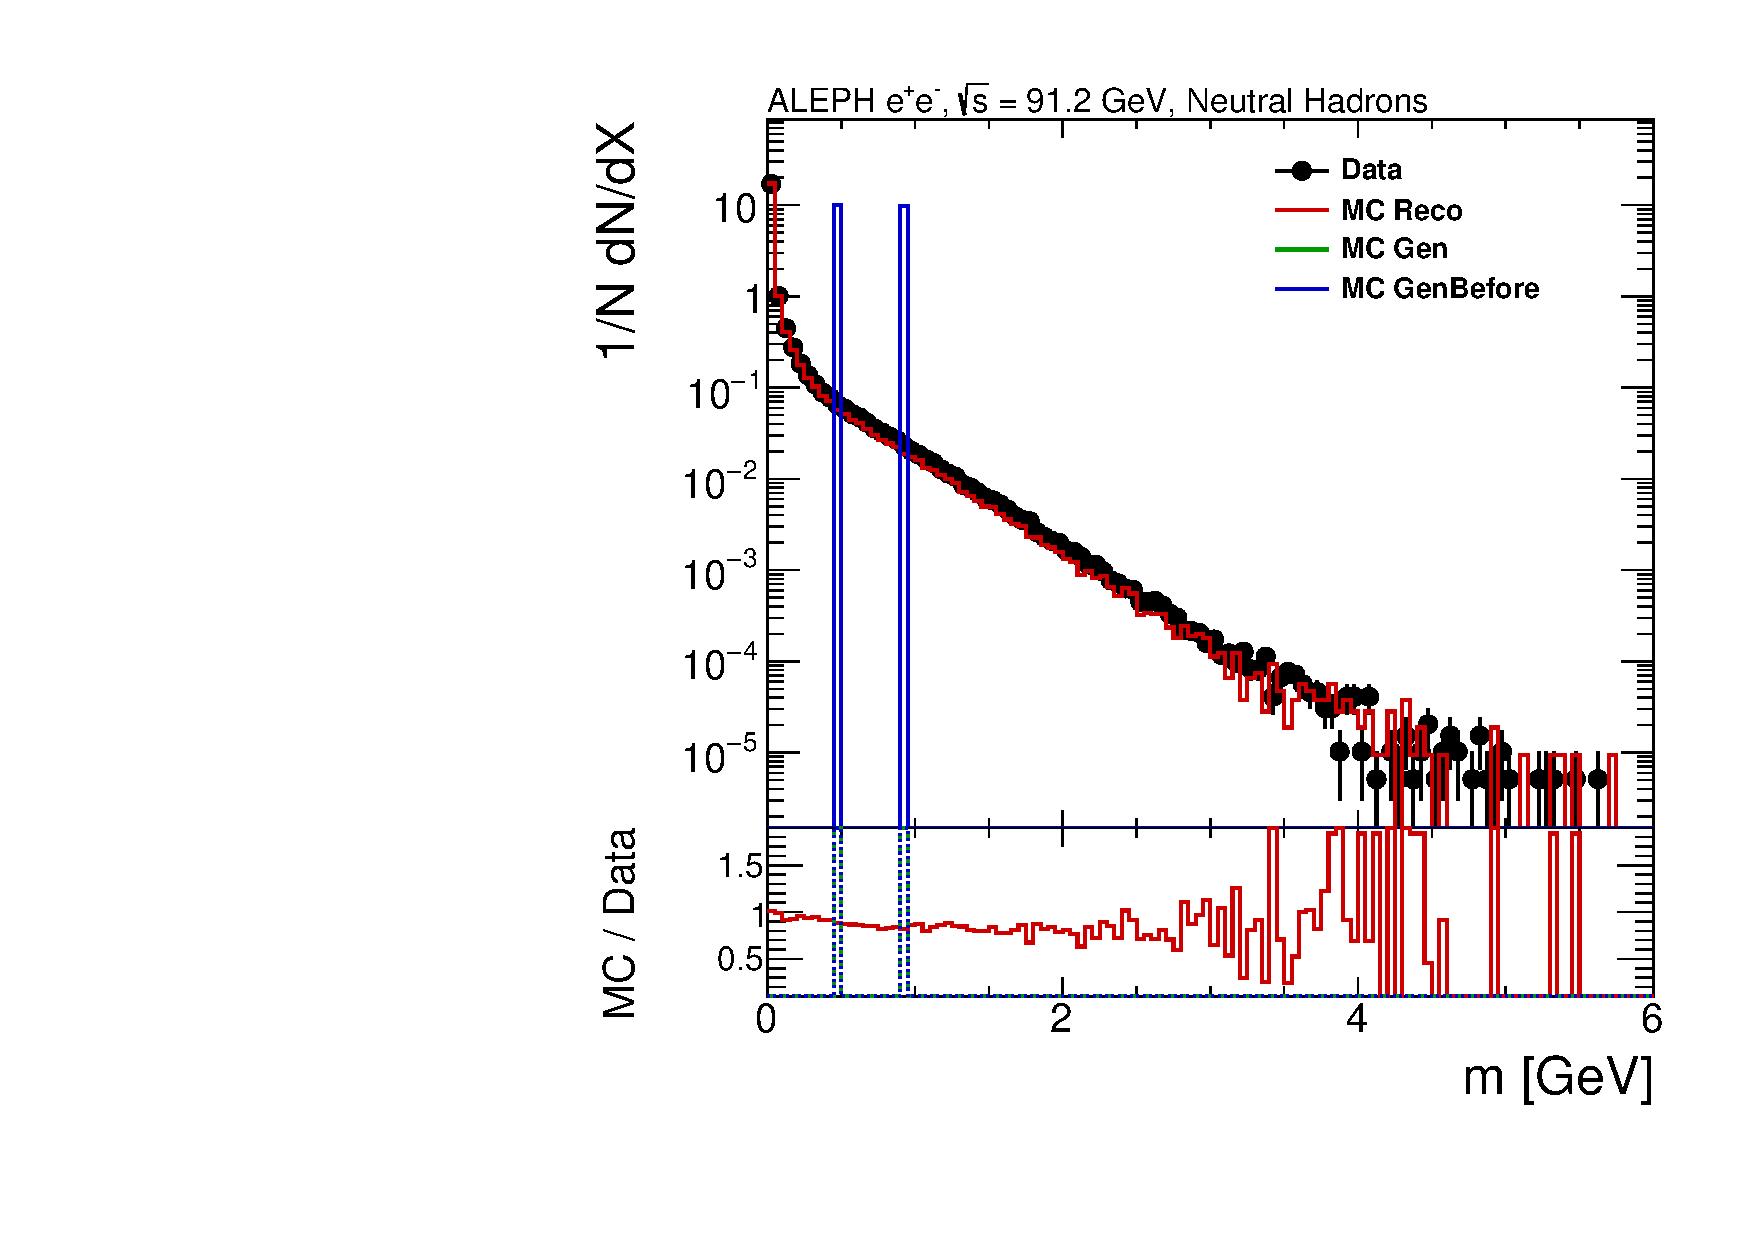
\includegraphics[width=0.325\textwidth]{../Studies/PreliminaryResult/2026-02-17_thrust_iter5/pwflag_kinematics/pwflag5_mass.pdf}
\caption{Complete \texttt{pwflag}=5 kinematic set.}
\label{fig:pwflag5_full}
\end{figure}

\noindent
Figure~\ref{fig:pwflag5_full} completes the neutral-hadron validation; this category is a key
input for neutral-response systematics propagated to the unfolded thrust result. This category is
typically softer and more sensitive to HCAL response and acceptance boundaries, so it is a direct
stress test of the neutral part of the thrust model. The remaining differences in low-statistics
tails are propagated through dedicated neutral-response and cross-check branches in the
experimental systematic program, rather than absorbed into ad hoc selections.
